\sectionthree{Cocke--Younger--Kasami Algorithm}
\begin{python0}
from solutions import *; clear()
\end{python0}

The
\defterm{Cocke--Younger--Kasami algorithm} (\defterm{CYK})
\tinysidebar{Cocke--Younger--Kasami algorithm\\CYK}
is an algorithm that determine if a string is generated by a CFG.
And if a string is generated by the CFG,
the algorithm can also give all the possible derivations.
In other words, it is a string parsing algorithm.
The time complexity is $O(n^3)$ where $n$ is the length of the string
(details below).
Later, faster algorithms were discovered.
For instance there is one with time complexity $O(n^{2.8})$.
The algorithm uses a very important technique in the design of algorithms
-- dynamic programming technique -- it builds up a solution by combining
solutions of subproblems of the given problem. 
Dynamic programming is an extremely important algorithm design technique
an is frequently used even in research.
(So it's not just a neat trick used in basic undergrad courses.)
One CYK dynamic programming example is definitely not enough.
See CISS358 for more details on dynamic programming.

Of course you can parse a string $w$ without CYK:
If $w$ is $\ep$, just check if $S$ is a nullable symbol.
Assuming the CFG is in Chomsky normal form, then every
production will increase the length of the sentential form
or replace a variable with a terminal.
So you need $|w|$ productions to introduce $|w|$ variables into the
derivation process and you need $|w|$ productions to replace the variables
with terminals. So there are at most $2|w|$ derivation steps, which is
of course finite.
So you just check every possible sequence of $2|w|$ productions starting
with $S$ and see if you can arrive at $w$.
Is this a good algorithm?
(Note sarcasm ...)

The main idea of CYK is very simple.
First we assume the grammar $G$ is in Chomsky normal form.
\sidebar{{\scriptsize Chomsky, Chomsky, Chomsky!}}
Now suppose our string $w$ has length $n$.
Let $w_{i,j}$ denote the substring of $w$ starting at position $i$ with 
length $j$.
The first position is $1$ and the last position is $n$.
The string $w$ is just
\[
w = w_{1,1} w_{2,1} w_{3,1} w_{4,1} \cdots w_{n,1}
\]

\begin{eg} 
Let $w = baabaa$. Then $w_{2,3} = aab$.
\end{eg}



\begin{ex} 
  \label{ex:some-decision1}
  \tinysidebar{\debug{exercises/{empty0/question.tex}}}
  \solutionlink{sol:some-decision1}
  \qed
\end{ex} 
\begin{python0}
from solutions import *
add(label="ex:some-decision1",
    srcfilename='exercises/some-decision1/answer.tex') 
\end{python0}


\newpage
First of all we can always determine if each $w_{i,1}$ can be
derived:
$A$ derives $w_{i,1}$ if and only if $A \rightarrow w_{i,1}$ is a production
(don't forget that we're assuming the grammar is in Chomsky Normal Form).
\sidebar{{\scriptsize Chomsky, Chomsky, Chomsky!}}


What about the general case?
How do you generate $w_{i,j}$?
This is a string starting at position $i$ and of length $j$.
What happens when you cut up the string?
Suppose you break it up into two strings $w_{i,j} = xy$.
Well, $x$ starts at the same index position in $w$ as $w_{i,j}$ right?
So it must be of the form
\[
x = w_{i,k}
\]
Since $x$ is a substring of $w_{i,j}$, it's length must be at most $j$.
Therefore $k \leq j$.
But let's assume that we really did cut up the string so that $y$ is not the 
empty string.
So $k < j$.
OK.
So we have
\[
  w_{i,j} = w_{i,k} y \text{ where } k < j
\]
Now let's think about $y$.

$y$ starts at position $i + k$, right?
And what is the length of $y$?
It's $|w| - |x|$ which is $j - k$.
So
\[
  y = w_{i + k, j - k}
\]
Viola.

Altogether, 
$w_{i,j}$ is the concatenation of $w_{i,k}$ and $w_{i+k, j-k}$
where $k < j$ (i.e., $k = 1, 2, \ldots, j - 1$):
\[
w_{i,j} = w_{i,k} w_{i+k, j-k}, \hskip 1cm (k = 1, 2, \ldots, j - 1)
\]
So what we'll do is
to find a variable, say $X$, deriving $w_{i,k}$:
\[
  X \istar w_{i,k}
\]
and 
another, say $Y$, deriving $w_{i+k, j-k}$
\[
  X \istar w_{i,k}
\]
for all the given $k$'s.
That means that $XY$ derives $w_{i,j}$
\[
  XY \istar w_{i,j}
\]
If the grammar is in Chomsky Normal Form, we will then look at the 
production rules to find a rule of the form $Z \rightarrow XY$.
If this is found, then $Z$ must derive $XY$ which derives $w_{i,j}$:
\[
  Z \implies XY \istar w_{i,j}
\]
That's the main idea.

The important thing to understand is that we are breaking down
out $w$ into two substrings exactly because the grammar is in
Chomsky Normal Form.
\sidebar{{\scriptsize Chomsky, Chomsky, Chomsky!}}
If the grammar has a production rule of the form
$Z \rightarrow WXY$, then our string $w$
might be derived through this production rule and in that case
we would have to break up $w$ into \textit{three} substrings
where $W$ derives the first, $X$ derives the second, and $Y$
derives the third.
The more variations there are in the right hand side of the
production rules of the grammar, the more cases
we would need to analyze to cover
all possibilities in the derivation process.
Get it?

Now let's go through an example ...


\newpage
\begin{eg}
Consider the grammar:
\begin{align*}
S &\rightarrow AB \st AC \\
A &\rightarrow BC \st a \\
B &\rightarrow CB \st b \\
C &\rightarrow AA \st b
\end{align*}
Note that this is already in Chomsky Normal Form.
Is $baaab$ generated by the grammar?
\end{eg}

\SOLUTION
For this example $w = baaab$.
We will systematically tabulate the variables deriving $w_{i,j}$.
The variables deriving $w_{i,j}$ will be placed at row $j$ and column $i$:
%-*-latex-*-
{\footnotesize \begin{Verbatim}[frame=single,fontsize=\small]
[student@localhost discrete-probability] python tossfaircoin2.py
experiment 0 ... outcome: TAIL
experiment 1 ... outcome: TAIL
experiment 2 ... outcome: TAIL
experiment 3 ... outcome: TAIL
experiment 4 ... outcome: TAIL
experiment 5 ... outcome: TAIL
experiment 6 ... outcome: HEAD
experiment 7 ... outcome: TAIL
experiment 8 ... outcome: TAIL
experiment 9 ... outcome: TAIL
experiment 10 ... outcome: TAIL
experiment 11 ... outcome: HEAD
experiment 12 ... outcome: HEAD
experiment 13 ... outcome: TAIL
experiment 14 ... outcome: HEAD
experiment 15 ... outcome: TAIL
experiment 16 ... outcome: TAIL
experiment 17 ... outcome: HEAD
experiment 18 ... outcome: HEAD
experiment 19 ... outcome: TAIL
number of experiments: 20
number of heads: 6
number of tails: 14
probability of getting head: 0.3
probability of getting tail: 0.7
\end{Verbatim}
}


\underline{First Row}:
We first work out $w_{i,1} = b$:
\begin{console}
12094
\end{console}


$b$ is derived only by $B \rightarrow b$ and $C \rightarrow b$:
\begin{center}
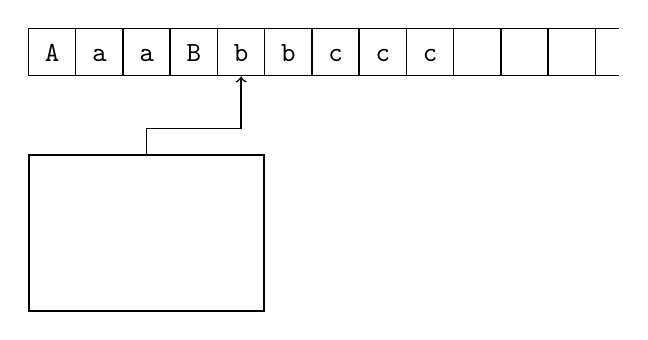
\begin{tikzpicture}

\draw (0.3, 0.3)
  node[draw, line width=0.02cm, , color=black,
       rounded corners=0cm, inner sep=0cm] {

\begin{minipage}[t][0.6cm]{0.6cm}
\mbox{}

\end{minipage}

};\draw (0.3, 0.3) node[color=black] {{\vphantom{AaaBbbccc$\BLANK$$\BLANK$$\BLANK$}\texttt{A}}};
\draw (0.8999999999999999, 0.3)
  node[draw, line width=0.02cm, , color=black,
       rounded corners=0cm, inner sep=0cm] {

\begin{minipage}[t][0.6cm]{0.6cm}
\mbox{}

\end{minipage}

};\draw (0.8999999999999999, 0.3) node[color=black] {{\vphantom{AaaBbbccc$\BLANK$$\BLANK$$\BLANK$}\texttt{a}}};
\draw (1.5, 0.3)
  node[draw, line width=0.02cm, , color=black,
       rounded corners=0cm, inner sep=0cm] {

\begin{minipage}[t][0.6cm]{0.6cm}
\mbox{}

\end{minipage}

};\draw (1.5, 0.3) node[color=black] {{\vphantom{AaaBbbccc$\BLANK$$\BLANK$$\BLANK$}\texttt{a}}};
\draw (2.0999999999999996, 0.3)
  node[draw, line width=0.02cm, , color=black,
       rounded corners=0cm, inner sep=0cm] {

\begin{minipage}[t][0.6cm]{0.6cm}
\mbox{}

\end{minipage}

};\draw (2.0999999999999996, 0.3) node[color=black] {{\vphantom{AaaBbbccc$\BLANK$$\BLANK$$\BLANK$}\texttt{B}}};
\draw (2.7, 0.3)
  node[draw, line width=0.02cm, , color=black,
       rounded corners=0cm, inner sep=0cm] {

\begin{minipage}[t][0.6cm]{0.6cm}
\mbox{}

\end{minipage}

};\draw (2.7, 0.3) node[color=black] {{\vphantom{AaaBbbccc$\BLANK$$\BLANK$$\BLANK$}\texttt{b}}};
\draw (3.3, 0.3)
  node[draw, line width=0.02cm, , color=black,
       rounded corners=0cm, inner sep=0cm] {

\begin{minipage}[t][0.6cm]{0.6cm}
\mbox{}

\end{minipage}

};\draw (3.3, 0.3) node[color=black] {{\vphantom{AaaBbbccc$\BLANK$$\BLANK$$\BLANK$}\texttt{b}}};
\draw (3.9000000000000004, 0.3)
  node[draw, line width=0.02cm, , color=black,
       rounded corners=0cm, inner sep=0cm] {

\begin{minipage}[t][0.6cm]{0.6cm}
\mbox{}

\end{minipage}

};\draw (3.9000000000000004, 0.3) node[color=black] {{\vphantom{AaaBbbccc$\BLANK$$\BLANK$$\BLANK$}\texttt{c}}};
\draw (4.5, 0.3)
  node[draw, line width=0.02cm, , color=black,
       rounded corners=0cm, inner sep=0cm] {

\begin{minipage}[t][0.6cm]{0.6cm}
\mbox{}

\end{minipage}

};\draw (4.5, 0.3) node[color=black] {{\vphantom{AaaBbbccc$\BLANK$$\BLANK$$\BLANK$}\texttt{c}}};
\draw (5.1, 0.3)
  node[draw, line width=0.02cm, , color=black,
       rounded corners=0cm, inner sep=0cm] {

\begin{minipage}[t][0.6cm]{0.6cm}
\mbox{}

\end{minipage}

};\draw (5.1, 0.3) node[color=black] {{\vphantom{AaaBbbccc$\BLANK$$\BLANK$$\BLANK$}\texttt{c}}};
\draw (5.699999999999999, 0.3)
  node[draw, line width=0.02cm, , color=black,
       rounded corners=0cm, inner sep=0cm] {

\begin{minipage}[t][0.6cm]{0.6cm}
\mbox{}

\end{minipage}

};\draw (5.699999999999999, 0.3) node[color=black] {{\vphantom{AaaBbbccc$\BLANK$$\BLANK$$\BLANK$}\texttt{$\BLANK$}}};
\draw (6.299999999999999, 0.3)
  node[draw, line width=0.02cm, , color=black,
       rounded corners=0cm, inner sep=0cm] {

\begin{minipage}[t][0.6cm]{0.6cm}
\mbox{}

\end{minipage}

};\draw (6.299999999999999, 0.3) node[color=black] {{\vphantom{AaaBbbccc$\BLANK$$\BLANK$$\BLANK$}\texttt{$\BLANK$}}};
\draw (6.899999999999999, 0.3)
  node[draw, line width=0.02cm, , color=black,
       rounded corners=0cm, inner sep=0cm] {

\begin{minipage}[t][0.6cm]{0.6cm}
\mbox{}

\end{minipage}

};\draw (6.899999999999999, 0.3) node[color=black] {{\vphantom{AaaBbbccc$\BLANK$$\BLANK$$\BLANK$}\texttt{$\BLANK$}}};\draw[line width=0.02cm,black] (7.1999999999999975,0.6) to  (7.499999999999998,0.6);
\draw[line width=0.02cm,black] (7.1999999999999975,0.0) to  (7.499999999999998,0.0);

\draw (1.5, -2.0)
  node[draw, line width=0.02cm, , color=black,
       rounded corners=0cm, inner sep=0cm] {

\begin{minipage}[t][1.98cm]{2.98cm}
\mbox{}

\end{minipage}

};\draw[line width=0.02cm,black,->] (1.5,-1) to  (1.5,-0.67) to  (2.7,-0.67) to  (2.7,-0.01);
\end{tikzpicture}

\end{center}


If you are interested in not just knowing if $baaaab$ is generated by the given grammar,
but you actually want to write down the derivation, it's helpful to include
some addition information for each variable in the cells.
I'll write these extra information in subscript.
I'll show you how these extra information will be used later.
%-*-latex-*-
\begin{Verbatim}[frame=single,fontsize=\small]
[student@localhost discrete-probability] python discrete-probrobability/game2.py
python: can't open file 'discrete-probrobability/game2.py': [Errno 2] No such fi
le or directory
\end{Verbatim}


In the above, the $B_b$ means \lq\lq $B$ will derive $b$''.

$a$ is derived by $A \rightarrow a$. This allows us to complete
the first row:
\begin{center}
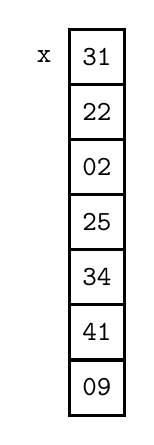
\begin{tikzpicture}

\draw (0.35, -0.35)
  node[draw, line width=0.04cm, , color=black,
       rounded corners=0cm, inner sep=0cm] {

\begin{minipage}[t][0.7cm]{0.7cm}
\mbox{}

\end{minipage}

};\draw (0.35, -0.35) node[color=black] {{\texttt{31}}};
\draw (0.35, -1.0499999999999998)
  node[draw, line width=0.04cm, , color=black,
       rounded corners=0cm, inner sep=0cm] {

\begin{minipage}[t][0.7cm]{0.7cm}
\mbox{}

\end{minipage}

};\draw (0.35, -1.0499999999999998) node[color=black] {{\texttt{22}}};
\draw (0.35, -1.7499999999999996)
  node[draw, line width=0.04cm, , color=black,
       rounded corners=0cm, inner sep=0cm] {

\begin{minipage}[t][0.7cm]{0.7cm}
\mbox{}

\end{minipage}

};\draw (0.35, -1.7499999999999996) node[color=black] {{\texttt{02}}};
\draw (0.35, -2.4499999999999997)
  node[draw, line width=0.04cm, , color=black,
       rounded corners=0cm, inner sep=0cm] {

\begin{minipage}[t][0.7cm]{0.7cm}
\mbox{}

\end{minipage}

};\draw (0.35, -2.4499999999999997) node[color=black] {{\texttt{25}}};
\draw (0.35, -3.15)
  node[draw, line width=0.04cm, , color=black,
       rounded corners=0cm, inner sep=0cm] {

\begin{minipage}[t][0.7cm]{0.7cm}
\mbox{}

\end{minipage}

};\draw (0.35, -3.15) node[color=black] {{\texttt{34}}};
\draw (0.35, -3.8499999999999996)
  node[draw, line width=0.04cm, , color=black,
       rounded corners=0cm, inner sep=0cm] {

\begin{minipage}[t][0.7cm]{0.7cm}
\mbox{}

\end{minipage}

};\draw (0.35, -3.8499999999999996) node[color=black] {{\texttt{41}}};
\draw (0.35, -4.550000000000001)
  node[draw, line width=0.04cm, , color=black,
       rounded corners=0cm, inner sep=0cm] {

\begin{minipage}[t][0.7cm]{0.7cm}
\mbox{}

\end{minipage}

};\draw (0.35, -4.550000000000001) node[color=black] {{\texttt{09}}};
\draw (-0.32, -0.35)
  node[draw=none, line width=0cm, , color=black,
       rounded corners=0cm, inner sep=0cm] {

\begin{minipage}[t][0.1cm]{0.1cm}
\mbox{}

\end{minipage}

};\draw (-0.32, -0.35) node[color=black] {\text{\texttt{x}}};
\end{tikzpicture}

\end{center}



In summary, to fill the first row, you need only to look at the
productions of the form $\langle variable \rangle \rightarrow \langle terminal
\rangle$.
(Don't memorize this. You should understand the goal and the math involved.)

\underline{Second Row}:
Now let's look at the $j=2, i=1$, i.e. $w_{1, 2}$:
\begin{console}[frame=single, , commandchars=~@$]
SLNode * p = phead;
while (p != NULL)
{
    std::cout << (*p) << std::endl;
    p = p->next();
}
\end{console}

and the output is this:
\begin{console}[frame=single,fontsize=\footnotesize]
[student@localhost linkedlist] g++ tmp12345678.cpp; ./a.out
<SLNode 0x7ffcf03deca0 key:2, next:0x7ffcf03decb0>
<SLNode 0x7ffcf03decb0 key:6, next:0x7ffcf03decc0>
<SLNode 0x7ffcf03decc0 key:4, next:0x7ffcf03decd0>
<SLNode 0x7ffcf03decd0 key:5, next:0>
\end{console}


Now
\[
w_{1,2} = w_{1,1} w_{2,1}
\]
(There's only one way to cut up $w_{1,2}$ into two proper substrings.)
But we already know that the variable deriving $w_{1,1}$ is at the $(1,1)$
entry in the table: it's either $B$ or $C$.
We also know that the variable deriving $w_{2,1}$ is at the $(1,2)$ entry;
this is $A$.
Therefore we want to find a variable $V$ such that 
\[
V \rightarrow BA
\]
or
\[
V \rightarrow CA
\]
is a production rule.
(Why do we consider only this scenario? Let's hear it ... 
\textit{ Chomsky, Chomsky, Chomsky, ...}
$BA$ and $CA$ does not appear on the right-hand side of the productions in 
the grammar.
READ THIS PARAGRAPH AGAIN!
So there are no such $V$s.
We will indicate this by putting $\emptyset$ at $(2, 1$).

The cells we looked at in order to fill the entry at $(2,1)$ are shaded.

\begin{longtable}{|r||r|r|r|r|r|}
\hline 
         & $0$ & $1$ & $2$ & $3$ & $\ldots$ \\ \hline \hline 
$x_0$    & 5   & 0   & 0   & 0   & ...      \\ \hline 
$x_1$    & 1   & 4   & 1   & 5   & ...      \\ \hline 
$x_2$    &     &     &     &     &          \\ \hline 
$x_3$    &     &     &     &     &          \\ \hline 
$\ldots$ &     &     &     &     &          \\ \hline 
\end{longtable}
        


Using the same idea, we can fill in the entry at $(2,2)$:
\begin{center}
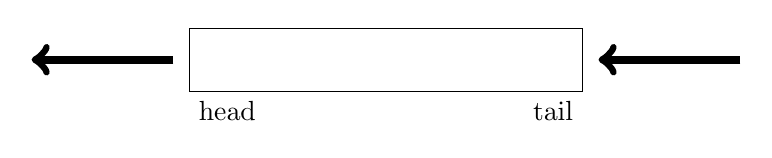
\begin{tikzpicture}

\draw (2.5, 0.4)
  node[draw, , , color=black,
       rounded corners=0cm, inner sep=0cm] {

\begin{minipage}[t][0.8cm]{5cm}
\mbox{}

\end{minipage}

};\draw[line width=0.1cm,black,->] (7,0.4) to  (5.2,0.4);
\draw[line width=0.1cm,black,->] (-0.2,0.4) to  (-2,0.4);

\node[anchor=north west] at (0,0)   {head};

\node[anchor=north east] at (5,0)   {tail};
\end{tikzpicture}

\end{center}


Here, $C$ derives $AA$.
The subscript data of $C$, i.e. $(1,2)$ and $(1,3)$, tells us that $C$
derives $XY$ where variable $X$ is in cell $(1,2)$ and
$Y$ is in cell $(1, 3)$.

Here's the table with row 2 completed:
\begin{center}
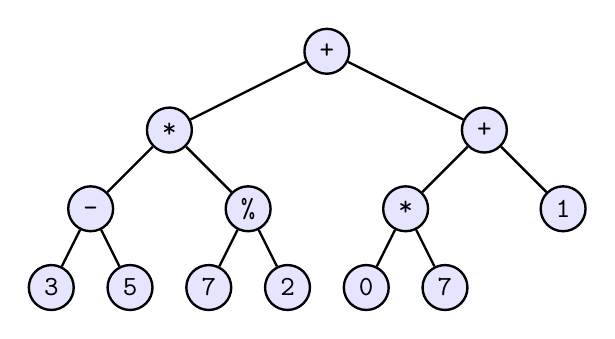
\begin{tikzpicture}

\fill[blue!10] (0.0, 0.0) circle (0.3);
\node [line width=0.03cm,black,minimum size=0.57cm,draw,circle] at (0.0,0.0)(+){};\draw (0.0, 0.0) node[color=black] {\texttt{+}};
\fill[blue!10] (-2.0, -1.0) circle (0.3);
\node [line width=0.03cm,black,minimum size=0.57cm,draw,circle] at (-2.0,-1.0)(*){};\draw (-2.0, -1.0) node[color=black] {\texttt{*}};
\fill[blue!10] (2.0, -1.0) circle (0.3);
\node [line width=0.03cm,black,minimum size=0.57cm,draw,circle] at (2.0,-1.0)(c){};\draw (2.0, -1.0) node[color=black] {\texttt{+}};
\fill[blue!10] (-3.0, -2.0) circle (0.3);
\node [line width=0.03cm,black,minimum size=0.57cm,draw,circle] at (-3.0,-2.0)(-){};\draw (-3.0, -2.0) node[color=black] {\texttt{-}};
\fill[blue!10] (-1.0, -2.0) circle (0.3);
\node [line width=0.03cm,black,minimum size=0.57cm,draw,circle] at (-1.0,-2.0)(e){};\draw (-1.0, -2.0) node[color=black] {\texttt{\%}};
\fill[blue!10] (1.0, -2.0) circle (0.3);
\node [line width=0.03cm,black,minimum size=0.57cm,draw,circle] at (1.0,-2.0)(f){};\draw (1.0, -2.0) node[color=black] {\texttt{*}};
\fill[blue!10] (3.0, -2.0) circle (0.3);
\node [line width=0.03cm,black,minimum size=0.57cm,draw,circle] at (3.0,-2.0)(1){};\draw (3.0, -2.0) node[color=black] {\texttt{1}};
\fill[blue!10] (-3.5, -3.0) circle (0.3);
\node [line width=0.03cm,black,minimum size=0.57cm,draw,circle] at (-3.5,-3.0)(3){};\draw (-3.5, -3.0) node[color=black] {\texttt{3}};
\fill[blue!10] (-2.5, -3.0) circle (0.3);
\node [line width=0.03cm,black,minimum size=0.57cm,draw,circle] at (-2.5,-3.0)(5){};\draw (-2.5, -3.0) node[color=black] {\texttt{5}};
\fill[blue!10] (-1.5, -3.0) circle (0.3);
\node [line width=0.03cm,black,minimum size=0.57cm,draw,circle] at (-1.5,-3.0)(z){};\draw (-1.5, -3.0) node[color=black] {\texttt{7}};
\fill[blue!10] (-0.5, -3.0) circle (0.3);
\node [line width=0.03cm,black,minimum size=0.57cm,draw,circle] at (-0.5,-3.0)(2){};\draw (-0.5, -3.0) node[color=black] {\texttt{2}};
\fill[blue!10] (0.5, -3.0) circle (0.3);
\node [line width=0.03cm,black,minimum size=0.57cm,draw,circle] at (0.5,-3.0)(0){};\draw (0.5, -3.0) node[color=black] {\texttt{0}};
\fill[blue!10] (1.5, -3.0) circle (0.3);
\node [line width=0.03cm,black,minimum size=0.57cm,draw,circle] at (1.5,-3.0)(7){};\draw (1.5, -3.0) node[color=black] {\texttt{7}};\draw[line width=0.03cm,black] (+) to  (*);
\draw[line width=0.03cm,black] (+) to  (c);
\draw[line width=0.03cm,black] (*) to  (-);
\draw[line width=0.03cm,black] (*) to  (e);
\draw[line width=0.03cm,black] (c) to  (f);
\draw[line width=0.03cm,black] (c) to  (1);
\draw[line width=0.03cm,black] (-) to  (3);
\draw[line width=0.03cm,black] (-) to  (5);
\draw[line width=0.03cm,black] (e) to  (z);
\draw[line width=0.03cm,black] (e) to  (2);
\draw[line width=0.03cm,black] (f) to  (0);
\draw[line width=0.03cm,black] (f) to  (7);
\end{tikzpicture}

\end{center}



Again, recall the aim: We're trying to fill the $(j,i)$ 
entry of the table with a variable that can derive $w_{i,j}$.

\underline{Third Row}:
Now we look at $j = 3, i = 1$:
\begin{center}
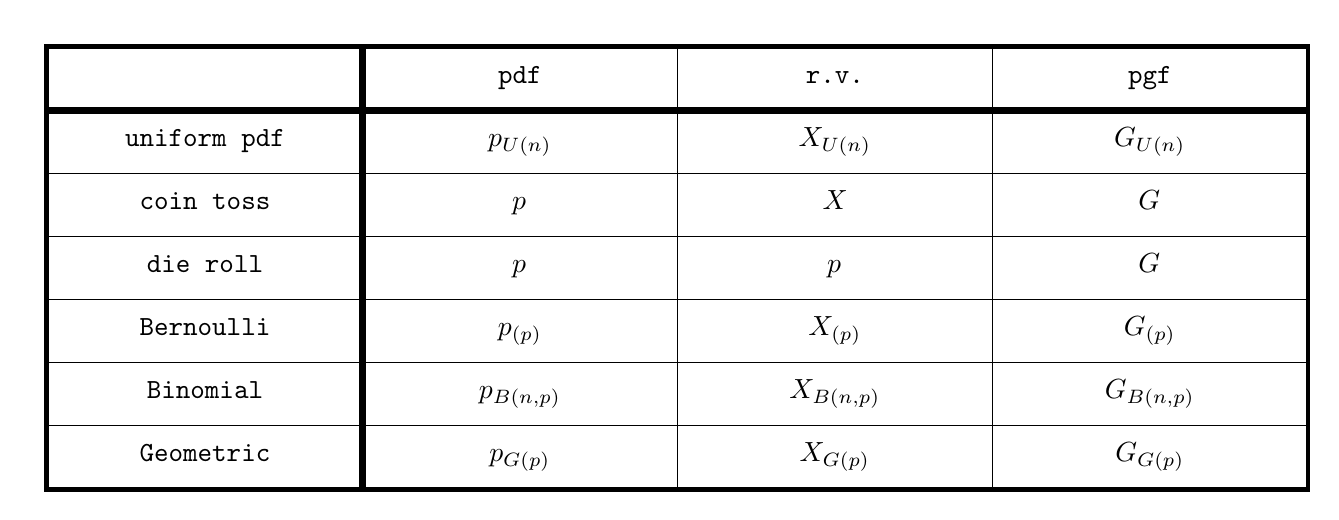
\begin{tikzpicture}

\draw (2.0, -0.4)
  node[draw, line width=0.02cm, , color=black,
       rounded corners=0cm, inner sep=0cm] {

\begin{minipage}[t][0.8cm]{4.0cm}
\mbox{}

\end{minipage}

};\draw (2.0, -0.4) node[color=black] {{\texttt{{\vphantom{pdfr.v.pgfuniform pdfcoin tossdie rollBernoulliBinomialGeometric$p_{U(n)}$$X_{U(n)}$$G_{U(n)}$$p_{\COIN}$$X_{\COIN}$$G_{\COIN}$$p_{\DIE}$$G_{\DIE}$$p_{\BERNOULLI(p)}$$X_{\BERNOULLI(p)}$$G_{\BERNOULLI(p)}$$p_{B(n,p)}$$X_{B(n,p)}$$G_{B(n,p)}$$p_{G(p)}$$X_{G(p)}$$G_{G(p)}$}}}}};\node[anchor=south] at (2.0,0.01) {};\node[anchor=east] at (-0.01,-0.4) {};
\draw (2.0, -0.4)
  node[draw, line width=0.06cm, , color=black,
       rounded corners=0cm, inner sep=0cm] {

\begin{minipage}[t][0.82cm]{4.02cm}
\mbox{}

\end{minipage}

};
\draw (6.0, -0.4)
  node[draw, line width=0.02cm, , color=black,
       rounded corners=0cm, inner sep=0cm] {

\begin{minipage}[t][0.8cm]{4.0cm}
\mbox{}

\end{minipage}

};\draw (6.0, -0.4) node[color=black] {{\texttt{{\vphantom{pdfr.v.pgfuniform pdfcoin tossdie rollBernoulliBinomialGeometric$p_{U(n)}$$X_{U(n)}$$G_{U(n)}$$p_{\COIN}$$X_{\COIN}$$G_{\COIN}$$p_{\DIE}$$G_{\DIE}$$p_{\BERNOULLI(p)}$$X_{\BERNOULLI(p)}$$G_{\BERNOULLI(p)}$$p_{B(n,p)}$$X_{B(n,p)}$$G_{B(n,p)}$$p_{G(p)}$$X_{G(p)}$$G_{G(p)}$}pdf}}}};
\draw (10.0, -0.4)
  node[draw, line width=0.02cm, , color=black,
       rounded corners=0cm, inner sep=0cm] {

\begin{minipage}[t][0.8cm]{4.0cm}
\mbox{}

\end{minipage}

};\draw (10.0, -0.4) node[color=black] {{\texttt{{\vphantom{pdfr.v.pgfuniform pdfcoin tossdie rollBernoulliBinomialGeometric$p_{U(n)}$$X_{U(n)}$$G_{U(n)}$$p_{\COIN}$$X_{\COIN}$$G_{\COIN}$$p_{\DIE}$$G_{\DIE}$$p_{\BERNOULLI(p)}$$X_{\BERNOULLI(p)}$$G_{\BERNOULLI(p)}$$p_{B(n,p)}$$X_{B(n,p)}$$G_{B(n,p)}$$p_{G(p)}$$X_{G(p)}$$G_{G(p)}$}r.v.}}}};
\draw (14.0, -0.4)
  node[draw, line width=0.02cm, , color=black,
       rounded corners=0cm, inner sep=0cm] {

\begin{minipage}[t][0.8cm]{4.0cm}
\mbox{}

\end{minipage}

};\draw (14.0, -0.4) node[color=black] {{\texttt{{\vphantom{pdfr.v.pgfuniform pdfcoin tossdie rollBernoulliBinomialGeometric$p_{U(n)}$$X_{U(n)}$$G_{U(n)}$$p_{\COIN}$$X_{\COIN}$$G_{\COIN}$$p_{\DIE}$$G_{\DIE}$$p_{\BERNOULLI(p)}$$X_{\BERNOULLI(p)}$$G_{\BERNOULLI(p)}$$p_{B(n,p)}$$X_{B(n,p)}$$G_{B(n,p)}$$p_{G(p)}$$X_{G(p)}$$G_{G(p)}$}pgf}}}};\node[anchor=south] at (6.0,0.01) {};\node[anchor=south] at (10.0,0.01) {};\node[anchor=south] at (14.0,0.01) {};\node[anchor=east] at (3.99,-0.4) {};
\draw (10.000000000000002, -0.4)
  node[draw, line width=0.06cm, , color=black,
       rounded corners=0cm, inner sep=0cm] {

\begin{minipage}[t][0.82cm]{12.02cm}
\mbox{}

\end{minipage}

};
\draw (2.0, -1.2000000000000002)
  node[draw, line width=0.02cm, , color=black,
       rounded corners=0cm, inner sep=0cm] {

\begin{minipage}[t][0.8cm]{4.0cm}
\mbox{}

\end{minipage}

};\draw (2.0, -1.2000000000000002) node[color=black] {{\texttt{{\vphantom{pdfr.v.pgfuniform pdfcoin tossdie rollBernoulliBinomialGeometric$p_{U(n)}$$X_{U(n)}$$G_{U(n)}$$p_{\COIN}$$X_{\COIN}$$G_{\COIN}$$p_{\DIE}$$G_{\DIE}$$p_{\BERNOULLI(p)}$$X_{\BERNOULLI(p)}$$G_{\BERNOULLI(p)}$$p_{B(n,p)}$$X_{B(n,p)}$$G_{B(n,p)}$$p_{G(p)}$$X_{G(p)}$$G_{G(p)}$}uniform pdf}}}};
\draw (2.0, -2.0)
  node[draw, line width=0.02cm, , color=black,
       rounded corners=0cm, inner sep=0cm] {

\begin{minipage}[t][0.8cm]{4.0cm}
\mbox{}

\end{minipage}

};\draw (2.0, -2.0) node[color=black] {{\texttt{{\vphantom{pdfr.v.pgfuniform pdfcoin tossdie rollBernoulliBinomialGeometric$p_{U(n)}$$X_{U(n)}$$G_{U(n)}$$p_{\COIN}$$X_{\COIN}$$G_{\COIN}$$p_{\DIE}$$G_{\DIE}$$p_{\BERNOULLI(p)}$$X_{\BERNOULLI(p)}$$G_{\BERNOULLI(p)}$$p_{B(n,p)}$$X_{B(n,p)}$$G_{B(n,p)}$$p_{G(p)}$$X_{G(p)}$$G_{G(p)}$}coin toss}}}};
\draw (2.0, -2.8000000000000003)
  node[draw, line width=0.02cm, , color=black,
       rounded corners=0cm, inner sep=0cm] {

\begin{minipage}[t][0.8cm]{4.0cm}
\mbox{}

\end{minipage}

};\draw (2.0, -2.8000000000000003) node[color=black] {{\texttt{{\vphantom{pdfr.v.pgfuniform pdfcoin tossdie rollBernoulliBinomialGeometric$p_{U(n)}$$X_{U(n)}$$G_{U(n)}$$p_{\COIN}$$X_{\COIN}$$G_{\COIN}$$p_{\DIE}$$G_{\DIE}$$p_{\BERNOULLI(p)}$$X_{\BERNOULLI(p)}$$G_{\BERNOULLI(p)}$$p_{B(n,p)}$$X_{B(n,p)}$$G_{B(n,p)}$$p_{G(p)}$$X_{G(p)}$$G_{G(p)}$}die roll}}}};
\draw (2.0, -3.6)
  node[draw, line width=0.02cm, , color=black,
       rounded corners=0cm, inner sep=0cm] {

\begin{minipage}[t][0.8cm]{4.0cm}
\mbox{}

\end{minipage}

};\draw (2.0, -3.6) node[color=black] {{\texttt{{\vphantom{pdfr.v.pgfuniform pdfcoin tossdie rollBernoulliBinomialGeometric$p_{U(n)}$$X_{U(n)}$$G_{U(n)}$$p_{\COIN}$$X_{\COIN}$$G_{\COIN}$$p_{\DIE}$$G_{\DIE}$$p_{\BERNOULLI(p)}$$X_{\BERNOULLI(p)}$$G_{\BERNOULLI(p)}$$p_{B(n,p)}$$X_{B(n,p)}$$G_{B(n,p)}$$p_{G(p)}$$X_{G(p)}$$G_{G(p)}$}Bernoulli}}}};
\draw (2.0, -4.4)
  node[draw, line width=0.02cm, , color=black,
       rounded corners=0cm, inner sep=0cm] {

\begin{minipage}[t][0.8cm]{4.0cm}
\mbox{}

\end{minipage}

};\draw (2.0, -4.4) node[color=black] {{\texttt{{\vphantom{pdfr.v.pgfuniform pdfcoin tossdie rollBernoulliBinomialGeometric$p_{U(n)}$$X_{U(n)}$$G_{U(n)}$$p_{\COIN}$$X_{\COIN}$$G_{\COIN}$$p_{\DIE}$$G_{\DIE}$$p_{\BERNOULLI(p)}$$X_{\BERNOULLI(p)}$$G_{\BERNOULLI(p)}$$p_{B(n,p)}$$X_{B(n,p)}$$G_{B(n,p)}$$p_{G(p)}$$X_{G(p)}$$G_{G(p)}$}Binomial}}}};
\draw (2.0, -5.199999999999999)
  node[draw, line width=0.02cm, , color=black,
       rounded corners=0cm, inner sep=0cm] {

\begin{minipage}[t][0.8cm]{4.0cm}
\mbox{}

\end{minipage}

};\draw (2.0, -5.199999999999999) node[color=black] {{\texttt{{\vphantom{pdfr.v.pgfuniform pdfcoin tossdie rollBernoulliBinomialGeometric$p_{U(n)}$$X_{U(n)}$$G_{U(n)}$$p_{\COIN}$$X_{\COIN}$$G_{\COIN}$$p_{\DIE}$$G_{\DIE}$$p_{\BERNOULLI(p)}$$X_{\BERNOULLI(p)}$$G_{\BERNOULLI(p)}$$p_{B(n,p)}$$X_{B(n,p)}$$G_{B(n,p)}$$p_{G(p)}$$X_{G(p)}$$G_{G(p)}$}Geometric}}}};\node[anchor=south] at (2.0,-0.79) {};\node[anchor=east] at (-0.01,-1.2000000000000002) {};\node[anchor=east] at (-0.01,-2.0000000000000004) {};\node[anchor=east] at (-0.01,-2.8000000000000003) {};\node[anchor=east] at (-0.01,-3.6) {};\node[anchor=east] at (-0.01,-4.4) {};\node[anchor=east] at (-0.01,-5.199999999999999) {};
\draw (2.0, -3.1999999999999997)
  node[draw, line width=0.06cm, , color=black,
       rounded corners=0cm, inner sep=0cm] {

\begin{minipage}[t][4.82cm]{4.02cm}
\mbox{}

\end{minipage}

};
\draw (6.0, -1.2000000000000002)
  node[draw, line width=0.02cm, , color=black,
       rounded corners=0cm, inner sep=0cm] {

\begin{minipage}[t][0.8cm]{4.0cm}
\mbox{}

\end{minipage}

};\draw (6.0, -1.2000000000000002) node[color=black] {{\texttt{{\vphantom{pdfr.v.pgfuniform pdfcoin tossdie rollBernoulliBinomialGeometric$p_{U(n)}$$X_{U(n)}$$G_{U(n)}$$p_{\COIN}$$X_{\COIN}$$G_{\COIN}$$p_{\DIE}$$G_{\DIE}$$p_{\BERNOULLI(p)}$$X_{\BERNOULLI(p)}$$G_{\BERNOULLI(p)}$$p_{B(n,p)}$$X_{B(n,p)}$$G_{B(n,p)}$$p_{G(p)}$$X_{G(p)}$$G_{G(p)}$}$p_{U(n)}$}}}};
\draw (10.0, -1.2000000000000002)
  node[draw, line width=0.02cm, , color=black,
       rounded corners=0cm, inner sep=0cm] {

\begin{minipage}[t][0.8cm]{4.0cm}
\mbox{}

\end{minipage}

};\draw (10.0, -1.2000000000000002) node[color=black] {{\texttt{{\vphantom{pdfr.v.pgfuniform pdfcoin tossdie rollBernoulliBinomialGeometric$p_{U(n)}$$X_{U(n)}$$G_{U(n)}$$p_{\COIN}$$X_{\COIN}$$G_{\COIN}$$p_{\DIE}$$G_{\DIE}$$p_{\BERNOULLI(p)}$$X_{\BERNOULLI(p)}$$G_{\BERNOULLI(p)}$$p_{B(n,p)}$$X_{B(n,p)}$$G_{B(n,p)}$$p_{G(p)}$$X_{G(p)}$$G_{G(p)}$}$X_{U(n)}$}}}};
\draw (14.0, -1.2000000000000002)
  node[draw, line width=0.02cm, , color=black,
       rounded corners=0cm, inner sep=0cm] {

\begin{minipage}[t][0.8cm]{4.0cm}
\mbox{}

\end{minipage}

};\draw (14.0, -1.2000000000000002) node[color=black] {{\texttt{{\vphantom{pdfr.v.pgfuniform pdfcoin tossdie rollBernoulliBinomialGeometric$p_{U(n)}$$X_{U(n)}$$G_{U(n)}$$p_{\COIN}$$X_{\COIN}$$G_{\COIN}$$p_{\DIE}$$G_{\DIE}$$p_{\BERNOULLI(p)}$$X_{\BERNOULLI(p)}$$G_{\BERNOULLI(p)}$$p_{B(n,p)}$$X_{B(n,p)}$$G_{B(n,p)}$$p_{G(p)}$$X_{G(p)}$$G_{G(p)}$}$G_{U(n)}$}}}};
\draw (6.0, -2.0)
  node[draw, line width=0.02cm, , color=black,
       rounded corners=0cm, inner sep=0cm] {

\begin{minipage}[t][0.8cm]{4.0cm}
\mbox{}

\end{minipage}

};\draw (6.0, -2.0) node[color=black] {{\texttt{{\vphantom{pdfr.v.pgfuniform pdfcoin tossdie rollBernoulliBinomialGeometric$p_{U(n)}$$X_{U(n)}$$G_{U(n)}$$p_{\COIN}$$X_{\COIN}$$G_{\COIN}$$p_{\DIE}$$G_{\DIE}$$p_{\BERNOULLI(p)}$$X_{\BERNOULLI(p)}$$G_{\BERNOULLI(p)}$$p_{B(n,p)}$$X_{B(n,p)}$$G_{B(n,p)}$$p_{G(p)}$$X_{G(p)}$$G_{G(p)}$}$p_{\COIN}$}}}};
\draw (10.0, -2.0)
  node[draw, line width=0.02cm, , color=black,
       rounded corners=0cm, inner sep=0cm] {

\begin{minipage}[t][0.8cm]{4.0cm}
\mbox{}

\end{minipage}

};\draw (10.0, -2.0) node[color=black] {{\texttt{{\vphantom{pdfr.v.pgfuniform pdfcoin tossdie rollBernoulliBinomialGeometric$p_{U(n)}$$X_{U(n)}$$G_{U(n)}$$p_{\COIN}$$X_{\COIN}$$G_{\COIN}$$p_{\DIE}$$G_{\DIE}$$p_{\BERNOULLI(p)}$$X_{\BERNOULLI(p)}$$G_{\BERNOULLI(p)}$$p_{B(n,p)}$$X_{B(n,p)}$$G_{B(n,p)}$$p_{G(p)}$$X_{G(p)}$$G_{G(p)}$}$X_{\COIN}$}}}};
\draw (14.0, -2.0)
  node[draw, line width=0.02cm, , color=black,
       rounded corners=0cm, inner sep=0cm] {

\begin{minipage}[t][0.8cm]{4.0cm}
\mbox{}

\end{minipage}

};\draw (14.0, -2.0) node[color=black] {{\texttt{{\vphantom{pdfr.v.pgfuniform pdfcoin tossdie rollBernoulliBinomialGeometric$p_{U(n)}$$X_{U(n)}$$G_{U(n)}$$p_{\COIN}$$X_{\COIN}$$G_{\COIN}$$p_{\DIE}$$G_{\DIE}$$p_{\BERNOULLI(p)}$$X_{\BERNOULLI(p)}$$G_{\BERNOULLI(p)}$$p_{B(n,p)}$$X_{B(n,p)}$$G_{B(n,p)}$$p_{G(p)}$$X_{G(p)}$$G_{G(p)}$}$G_{\COIN}$}}}};
\draw (6.0, -2.8000000000000003)
  node[draw, line width=0.02cm, , color=black,
       rounded corners=0cm, inner sep=0cm] {

\begin{minipage}[t][0.8cm]{4.0cm}
\mbox{}

\end{minipage}

};\draw (6.0, -2.8000000000000003) node[color=black] {{\texttt{{\vphantom{pdfr.v.pgfuniform pdfcoin tossdie rollBernoulliBinomialGeometric$p_{U(n)}$$X_{U(n)}$$G_{U(n)}$$p_{\COIN}$$X_{\COIN}$$G_{\COIN}$$p_{\DIE}$$G_{\DIE}$$p_{\BERNOULLI(p)}$$X_{\BERNOULLI(p)}$$G_{\BERNOULLI(p)}$$p_{B(n,p)}$$X_{B(n,p)}$$G_{B(n,p)}$$p_{G(p)}$$X_{G(p)}$$G_{G(p)}$}$p_{\DIE}$}}}};
\draw (10.0, -2.8000000000000003)
  node[draw, line width=0.02cm, , color=black,
       rounded corners=0cm, inner sep=0cm] {

\begin{minipage}[t][0.8cm]{4.0cm}
\mbox{}

\end{minipage}

};\draw (10.0, -2.8000000000000003) node[color=black] {{\texttt{{\vphantom{pdfr.v.pgfuniform pdfcoin tossdie rollBernoulliBinomialGeometric$p_{U(n)}$$X_{U(n)}$$G_{U(n)}$$p_{\COIN}$$X_{\COIN}$$G_{\COIN}$$p_{\DIE}$$G_{\DIE}$$p_{\BERNOULLI(p)}$$X_{\BERNOULLI(p)}$$G_{\BERNOULLI(p)}$$p_{B(n,p)}$$X_{B(n,p)}$$G_{B(n,p)}$$p_{G(p)}$$X_{G(p)}$$G_{G(p)}$}$p_{\DIE}$}}}};
\draw (14.0, -2.8000000000000003)
  node[draw, line width=0.02cm, , color=black,
       rounded corners=0cm, inner sep=0cm] {

\begin{minipage}[t][0.8cm]{4.0cm}
\mbox{}

\end{minipage}

};\draw (14.0, -2.8000000000000003) node[color=black] {{\texttt{{\vphantom{pdfr.v.pgfuniform pdfcoin tossdie rollBernoulliBinomialGeometric$p_{U(n)}$$X_{U(n)}$$G_{U(n)}$$p_{\COIN}$$X_{\COIN}$$G_{\COIN}$$p_{\DIE}$$G_{\DIE}$$p_{\BERNOULLI(p)}$$X_{\BERNOULLI(p)}$$G_{\BERNOULLI(p)}$$p_{B(n,p)}$$X_{B(n,p)}$$G_{B(n,p)}$$p_{G(p)}$$X_{G(p)}$$G_{G(p)}$}$G_{\DIE}$}}}};
\draw (6.0, -3.6)
  node[draw, line width=0.02cm, , color=black,
       rounded corners=0cm, inner sep=0cm] {

\begin{minipage}[t][0.8cm]{4.0cm}
\mbox{}

\end{minipage}

};\draw (6.0, -3.6) node[color=black] {{\texttt{{\vphantom{pdfr.v.pgfuniform pdfcoin tossdie rollBernoulliBinomialGeometric$p_{U(n)}$$X_{U(n)}$$G_{U(n)}$$p_{\COIN}$$X_{\COIN}$$G_{\COIN}$$p_{\DIE}$$G_{\DIE}$$p_{\BERNOULLI(p)}$$X_{\BERNOULLI(p)}$$G_{\BERNOULLI(p)}$$p_{B(n,p)}$$X_{B(n,p)}$$G_{B(n,p)}$$p_{G(p)}$$X_{G(p)}$$G_{G(p)}$}$p_{\BERNOULLI(p)}$}}}};
\draw (10.0, -3.6)
  node[draw, line width=0.02cm, , color=black,
       rounded corners=0cm, inner sep=0cm] {

\begin{minipage}[t][0.8cm]{4.0cm}
\mbox{}

\end{minipage}

};\draw (10.0, -3.6) node[color=black] {{\texttt{{\vphantom{pdfr.v.pgfuniform pdfcoin tossdie rollBernoulliBinomialGeometric$p_{U(n)}$$X_{U(n)}$$G_{U(n)}$$p_{\COIN}$$X_{\COIN}$$G_{\COIN}$$p_{\DIE}$$G_{\DIE}$$p_{\BERNOULLI(p)}$$X_{\BERNOULLI(p)}$$G_{\BERNOULLI(p)}$$p_{B(n,p)}$$X_{B(n,p)}$$G_{B(n,p)}$$p_{G(p)}$$X_{G(p)}$$G_{G(p)}$}$X_{\BERNOULLI(p)}$}}}};
\draw (14.0, -3.6)
  node[draw, line width=0.02cm, , color=black,
       rounded corners=0cm, inner sep=0cm] {

\begin{minipage}[t][0.8cm]{4.0cm}
\mbox{}

\end{minipage}

};\draw (14.0, -3.6) node[color=black] {{\texttt{{\vphantom{pdfr.v.pgfuniform pdfcoin tossdie rollBernoulliBinomialGeometric$p_{U(n)}$$X_{U(n)}$$G_{U(n)}$$p_{\COIN}$$X_{\COIN}$$G_{\COIN}$$p_{\DIE}$$G_{\DIE}$$p_{\BERNOULLI(p)}$$X_{\BERNOULLI(p)}$$G_{\BERNOULLI(p)}$$p_{B(n,p)}$$X_{B(n,p)}$$G_{B(n,p)}$$p_{G(p)}$$X_{G(p)}$$G_{G(p)}$}$G_{\BERNOULLI(p)}$}}}};
\draw (6.0, -4.4)
  node[draw, line width=0.02cm, , color=black,
       rounded corners=0cm, inner sep=0cm] {

\begin{minipage}[t][0.8cm]{4.0cm}
\mbox{}

\end{minipage}

};\draw (6.0, -4.4) node[color=black] {{\texttt{{\vphantom{pdfr.v.pgfuniform pdfcoin tossdie rollBernoulliBinomialGeometric$p_{U(n)}$$X_{U(n)}$$G_{U(n)}$$p_{\COIN}$$X_{\COIN}$$G_{\COIN}$$p_{\DIE}$$G_{\DIE}$$p_{\BERNOULLI(p)}$$X_{\BERNOULLI(p)}$$G_{\BERNOULLI(p)}$$p_{B(n,p)}$$X_{B(n,p)}$$G_{B(n,p)}$$p_{G(p)}$$X_{G(p)}$$G_{G(p)}$}$p_{B(n,p)}$}}}};
\draw (10.0, -4.4)
  node[draw, line width=0.02cm, , color=black,
       rounded corners=0cm, inner sep=0cm] {

\begin{minipage}[t][0.8cm]{4.0cm}
\mbox{}

\end{minipage}

};\draw (10.0, -4.4) node[color=black] {{\texttt{{\vphantom{pdfr.v.pgfuniform pdfcoin tossdie rollBernoulliBinomialGeometric$p_{U(n)}$$X_{U(n)}$$G_{U(n)}$$p_{\COIN}$$X_{\COIN}$$G_{\COIN}$$p_{\DIE}$$G_{\DIE}$$p_{\BERNOULLI(p)}$$X_{\BERNOULLI(p)}$$G_{\BERNOULLI(p)}$$p_{B(n,p)}$$X_{B(n,p)}$$G_{B(n,p)}$$p_{G(p)}$$X_{G(p)}$$G_{G(p)}$}$X_{B(n,p)}$}}}};
\draw (14.0, -4.4)
  node[draw, line width=0.02cm, , color=black,
       rounded corners=0cm, inner sep=0cm] {

\begin{minipage}[t][0.8cm]{4.0cm}
\mbox{}

\end{minipage}

};\draw (14.0, -4.4) node[color=black] {{\texttt{{\vphantom{pdfr.v.pgfuniform pdfcoin tossdie rollBernoulliBinomialGeometric$p_{U(n)}$$X_{U(n)}$$G_{U(n)}$$p_{\COIN}$$X_{\COIN}$$G_{\COIN}$$p_{\DIE}$$G_{\DIE}$$p_{\BERNOULLI(p)}$$X_{\BERNOULLI(p)}$$G_{\BERNOULLI(p)}$$p_{B(n,p)}$$X_{B(n,p)}$$G_{B(n,p)}$$p_{G(p)}$$X_{G(p)}$$G_{G(p)}$}$G_{B(n,p)}$}}}};
\draw (6.0, -5.199999999999999)
  node[draw, line width=0.02cm, , color=black,
       rounded corners=0cm, inner sep=0cm] {

\begin{minipage}[t][0.8cm]{4.0cm}
\mbox{}

\end{minipage}

};\draw (6.0, -5.199999999999999) node[color=black] {{\texttt{{\vphantom{pdfr.v.pgfuniform pdfcoin tossdie rollBernoulliBinomialGeometric$p_{U(n)}$$X_{U(n)}$$G_{U(n)}$$p_{\COIN}$$X_{\COIN}$$G_{\COIN}$$p_{\DIE}$$G_{\DIE}$$p_{\BERNOULLI(p)}$$X_{\BERNOULLI(p)}$$G_{\BERNOULLI(p)}$$p_{B(n,p)}$$X_{B(n,p)}$$G_{B(n,p)}$$p_{G(p)}$$X_{G(p)}$$G_{G(p)}$}$p_{G(p)}$}}}};
\draw (10.0, -5.199999999999999)
  node[draw, line width=0.02cm, , color=black,
       rounded corners=0cm, inner sep=0cm] {

\begin{minipage}[t][0.8cm]{4.0cm}
\mbox{}

\end{minipage}

};\draw (10.0, -5.199999999999999) node[color=black] {{\texttt{{\vphantom{pdfr.v.pgfuniform pdfcoin tossdie rollBernoulliBinomialGeometric$p_{U(n)}$$X_{U(n)}$$G_{U(n)}$$p_{\COIN}$$X_{\COIN}$$G_{\COIN}$$p_{\DIE}$$G_{\DIE}$$p_{\BERNOULLI(p)}$$X_{\BERNOULLI(p)}$$G_{\BERNOULLI(p)}$$p_{B(n,p)}$$X_{B(n,p)}$$G_{B(n,p)}$$p_{G(p)}$$X_{G(p)}$$G_{G(p)}$}$X_{G(p)}$}}}};
\draw (14.0, -5.199999999999999)
  node[draw, line width=0.02cm, , color=black,
       rounded corners=0cm, inner sep=0cm] {

\begin{minipage}[t][0.8cm]{4.0cm}
\mbox{}

\end{minipage}

};\draw (14.0, -5.199999999999999) node[color=black] {{\texttt{{\vphantom{pdfr.v.pgfuniform pdfcoin tossdie rollBernoulliBinomialGeometric$p_{U(n)}$$X_{U(n)}$$G_{U(n)}$$p_{\COIN}$$X_{\COIN}$$G_{\COIN}$$p_{\DIE}$$G_{\DIE}$$p_{\BERNOULLI(p)}$$X_{\BERNOULLI(p)}$$G_{\BERNOULLI(p)}$$p_{B(n,p)}$$X_{B(n,p)}$$G_{B(n,p)}$$p_{G(p)}$$X_{G(p)}$$G_{G(p)}$}$G_{G(p)}$}}}};\node[anchor=south] at (6.0,-0.79) {};\node[anchor=south] at (10.0,-0.79) {};\node[anchor=south] at (14.0,-0.79) {};\node[anchor=east] at (3.99,-1.2000000000000002) {};\node[anchor=east] at (3.99,-2.0000000000000004) {};\node[anchor=east] at (3.99,-2.8000000000000003) {};\node[anchor=east] at (3.99,-3.6) {};\node[anchor=east] at (3.99,-4.4) {};\node[anchor=east] at (3.99,-5.199999999999999) {};
\draw (10.000000000000002, -3.1999999999999997)
  node[draw, line width=0.06cm, , color=black,
       rounded corners=0cm, inner sep=0cm] {

\begin{minipage}[t][4.82cm]{12.02cm}
\mbox{}

\end{minipage}

};
\end{tikzpicture}

\end{center}


We want to to find a variable $V$ that derives $w_{1,3}$.
Recall from the above that we want to make use of previous results.
The following are the possible ways of breaking up $w_{1,3}$:
\[
w_{1,1}w_{2,2} \hskip 1cm \text{or} \hskip 1cm w_{1,2} w_{3,1}
\]
In other words if $w_{1, 3}$ is $xyz$ then the two ways to break up 
$w_{1,3}$ into two proper substrings are:
\[
x \cdot yz \hskip 1cm \text{or} \hskip 1cm  xy \cdot z
\]
We already know that the variable deriving $w_{1,1}$ is in the
entry at $(1,1)$ of the table: it's $B$ or $C$.
For $w_{2,2}$, just look at the entry at $(2,2)$; $C$ derives 
$w_{2,2}$.
Therefore $BC$ and $CC$ derives $w_{1,1}w_{2,2}$ which is just 
$w_{1, 3}$.
Now we want to find $V$ that derives $BC$ or $CC$:
\[
  V \implies XY \text{ where } X \in \{B, C\} \text{ and } Y \in \{C\} 
\]
and enter that
into the $(3,1)$ entry of the table.
Checking the grammar, we see that only $A$ can do this.
Therefore we have
\begin{center}
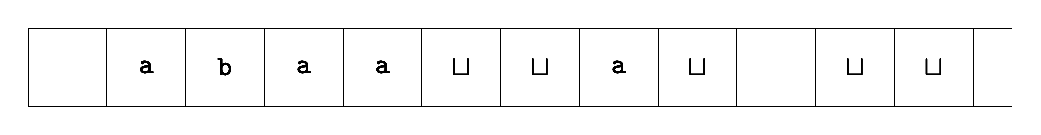
\begin{tikzpicture}

\draw (0.49999999999999994, 0.49999999999999994)
  node[draw, line width=0.01cm, , color=black,
       rounded corners=0cm, inner sep=0cm] {

\begin{minipage}[t][1.0cm]{1.0cm}
\mbox{}

\end{minipage}

};\draw (0.49999999999999994, 0.49999999999999994) node[color=black] {\texttt{\DOLLAR}};
\draw (1.5, 0.49999999999999994)
  node[draw, line width=0.01cm, , color=black,
       rounded corners=0cm, inner sep=0cm] {

\begin{minipage}[t][1.0cm]{1.0cm}
\mbox{}

\end{minipage}

};\draw (1.5, 0.49999999999999994) node[color=black] {\texttt{a}};
\draw (2.5, 0.49999999999999994)
  node[draw, line width=0.01cm, , color=black,
       rounded corners=0cm, inner sep=0cm] {

\begin{minipage}[t][1.0cm]{1.0cm}
\mbox{}

\end{minipage}

};\draw (2.5, 0.49999999999999994) node[color=black] {\texttt{b}};
\draw (3.5, 0.49999999999999994)
  node[draw, line width=0.01cm, , color=black,
       rounded corners=0cm, inner sep=0cm] {

\begin{minipage}[t][1.0cm]{1.0cm}
\mbox{}

\end{minipage}

};\draw (3.5, 0.49999999999999994) node[color=black] {\texttt{a}};
\draw (4.5, 0.49999999999999994)
  node[draw, line width=0.01cm, , color=black,
       rounded corners=0cm, inner sep=0cm] {

\begin{minipage}[t][1.0cm]{1.0cm}
\mbox{}

\end{minipage}

};\draw (4.5, 0.49999999999999994) node[color=black] {\texttt{a}};
\draw (5.5, 0.49999999999999994)
  node[draw, line width=0.01cm, , color=black,
       rounded corners=0cm, inner sep=0cm] {

\begin{minipage}[t][1.0cm]{1.0cm}
\mbox{}

\end{minipage}

};\draw (5.5, 0.49999999999999994) node[color=black] {\texttt{$\sqcup$}};
\draw (6.5, 0.49999999999999994)
  node[draw, line width=0.01cm, , color=black,
       rounded corners=0cm, inner sep=0cm] {

\begin{minipage}[t][1.0cm]{1.0cm}
\mbox{}

\end{minipage}

};\draw (6.5, 0.49999999999999994) node[color=black] {\texttt{$\sqcup$}};
\draw (7.5, 0.49999999999999994)
  node[draw, line width=0.01cm, , color=black,
       rounded corners=0cm, inner sep=0cm] {

\begin{minipage}[t][1.0cm]{1.0cm}
\mbox{}

\end{minipage}

};\draw (7.5, 0.49999999999999994) node[color=black] {\texttt{a}};
\draw (8.5, 0.49999999999999994)
  node[draw, line width=0.01cm, , color=black,
       rounded corners=0cm, inner sep=0cm] {

\begin{minipage}[t][1.0cm]{1.0cm}
\mbox{}

\end{minipage}

};\draw (8.5, 0.49999999999999994) node[color=black] {\texttt{$\sqcup$}};
\draw (9.5, 0.49999999999999994)
  node[draw, line width=0.01cm, , color=black,
       rounded corners=0cm, inner sep=0cm] {

\begin{minipage}[t][1.0cm]{1.0cm}
\mbox{}

\end{minipage}

};\draw (9.5, 0.49999999999999994) node[color=black] {\texttt{$\EOT$}};
\draw (10.5, 0.49999999999999994)
  node[draw, line width=0.01cm, , color=black,
       rounded corners=0cm, inner sep=0cm] {

\begin{minipage}[t][1.0cm]{1.0cm}
\mbox{}

\end{minipage}

};\draw (10.5, 0.49999999999999994) node[color=black] {\texttt{$\sqcup$}};
\draw (11.5, 0.49999999999999994)
  node[draw, line width=0.01cm, , color=black,
       rounded corners=0cm, inner sep=0cm] {

\begin{minipage}[t][1.0cm]{1.0cm}
\mbox{}

\end{minipage}

};\draw (11.5, 0.49999999999999994) node[color=black] {\texttt{$\sqcup$}};
\draw (0.49999999999999994, 0.49999999999999994)
  node[draw, line width=0.01cm, , color=black,
       rounded corners=0cm, inner sep=0cm] {

\begin{minipage}[t][1.0cm]{1.0cm}
\mbox{}

\end{minipage}

};\draw (0.49999999999999994, 0.49999999999999994) node[color=black] {\texttt{\DOLLAR}};
\draw (1.5, 0.49999999999999994)
  node[draw, line width=0.01cm, , color=black,
       rounded corners=0cm, inner sep=0cm] {

\begin{minipage}[t][1.0cm]{1.0cm}
\mbox{}

\end{minipage}

};\draw (1.5, 0.49999999999999994) node[color=black] {\texttt{a}};
\draw (2.5, 0.49999999999999994)
  node[draw, line width=0.01cm, , color=black,
       rounded corners=0cm, inner sep=0cm] {

\begin{minipage}[t][1.0cm]{1.0cm}
\mbox{}

\end{minipage}

};\draw (2.5, 0.49999999999999994) node[color=black] {\texttt{b}};
\draw (3.5, 0.49999999999999994)
  node[draw, line width=0.01cm, , color=black,
       rounded corners=0cm, inner sep=0cm] {

\begin{minipage}[t][1.0cm]{1.0cm}
\mbox{}

\end{minipage}

};\draw (3.5, 0.49999999999999994) node[color=black] {\texttt{a}};
\draw (4.5, 0.49999999999999994)
  node[draw, line width=0.01cm, , color=black,
       rounded corners=0cm, inner sep=0cm] {

\begin{minipage}[t][1.0cm]{1.0cm}
\mbox{}

\end{minipage}

};\draw (4.5, 0.49999999999999994) node[color=black] {\texttt{a}};
\draw (5.5, 0.49999999999999994)
  node[draw, line width=0.01cm, , color=black,
       rounded corners=0cm, inner sep=0cm] {

\begin{minipage}[t][1.0cm]{1.0cm}
\mbox{}

\end{minipage}

};\draw (5.5, 0.49999999999999994) node[color=black] {\texttt{$\sqcup$}};
\draw (6.5, 0.49999999999999994)
  node[draw, line width=0.01cm, , color=black,
       rounded corners=0cm, inner sep=0cm] {

\begin{minipage}[t][1.0cm]{1.0cm}
\mbox{}

\end{minipage}

};\draw (6.5, 0.49999999999999994) node[color=black] {\texttt{$\sqcup$}};
\draw (7.5, 0.49999999999999994)
  node[draw, line width=0.01cm, , color=black,
       rounded corners=0cm, inner sep=0cm] {

\begin{minipage}[t][1.0cm]{1.0cm}
\mbox{}

\end{minipage}

};\draw (7.5, 0.49999999999999994) node[color=black] {\texttt{a}};
\draw (8.5, 0.49999999999999994)
  node[draw, line width=0.01cm, , color=black,
       rounded corners=0cm, inner sep=0cm] {

\begin{minipage}[t][1.0cm]{1.0cm}
\mbox{}

\end{minipage}

};\draw (8.5, 0.49999999999999994) node[color=black] {\texttt{$\sqcup$}};
\draw (9.5, 0.49999999999999994)
  node[draw, line width=0.01cm, , color=black,
       rounded corners=0cm, inner sep=0cm] {

\begin{minipage}[t][1.0cm]{1.0cm}
\mbox{}

\end{minipage}

};\draw (9.5, 0.49999999999999994) node[color=black] {\texttt{$\EOT$}};
\draw (10.5, 0.49999999999999994)
  node[draw, line width=0.01cm, , color=black,
       rounded corners=0cm, inner sep=0cm] {

\begin{minipage}[t][1.0cm]{1.0cm}
\mbox{}

\end{minipage}

};\draw (10.5, 0.49999999999999994) node[color=black] {\texttt{$\sqcup$}};
\draw (11.5, 0.49999999999999994)
  node[draw, line width=0.01cm, , color=black,
       rounded corners=0cm, inner sep=0cm] {

\begin{minipage}[t][1.0cm]{1.0cm}
\mbox{}

\end{minipage}

};\draw (11.5, 0.49999999999999994) node[color=black] {\texttt{$\sqcup$}};
\draw (0.49999999999999994, 0.49999999999999994)
  node[draw, line width=0.01cm, , color=black,
       rounded corners=0cm, inner sep=0cm] {

\begin{minipage}[t][1.0cm]{1.0cm}
\mbox{}

\end{minipage}

};\draw (0.49999999999999994, 0.49999999999999994) node[color=black] {\texttt{\DOLLAR}};
\draw (1.5, 0.49999999999999994)
  node[draw, line width=0.01cm, , color=black,
       rounded corners=0cm, inner sep=0cm] {

\begin{minipage}[t][1.0cm]{1.0cm}
\mbox{}

\end{minipage}

};\draw (1.5, 0.49999999999999994) node[color=black] {\texttt{a}};
\draw (2.5, 0.49999999999999994)
  node[draw, line width=0.01cm, , color=black,
       rounded corners=0cm, inner sep=0cm] {

\begin{minipage}[t][1.0cm]{1.0cm}
\mbox{}

\end{minipage}

};\draw (2.5, 0.49999999999999994) node[color=black] {\texttt{b}};
\draw (3.5, 0.49999999999999994)
  node[draw, line width=0.01cm, , color=black,
       rounded corners=0cm, inner sep=0cm] {

\begin{minipage}[t][1.0cm]{1.0cm}
\mbox{}

\end{minipage}

};\draw (3.5, 0.49999999999999994) node[color=black] {\texttt{a}};
\draw (4.5, 0.49999999999999994)
  node[draw, line width=0.01cm, , color=black,
       rounded corners=0cm, inner sep=0cm] {

\begin{minipage}[t][1.0cm]{1.0cm}
\mbox{}

\end{minipage}

};\draw (4.5, 0.49999999999999994) node[color=black] {\texttt{a}};
\draw (5.5, 0.49999999999999994)
  node[draw, line width=0.01cm, , color=black,
       rounded corners=0cm, inner sep=0cm] {

\begin{minipage}[t][1.0cm]{1.0cm}
\mbox{}

\end{minipage}

};\draw (5.5, 0.49999999999999994) node[color=black] {\texttt{$\sqcup$}};
\draw (6.5, 0.49999999999999994)
  node[draw, line width=0.01cm, , color=black,
       rounded corners=0cm, inner sep=0cm] {

\begin{minipage}[t][1.0cm]{1.0cm}
\mbox{}

\end{minipage}

};\draw (6.5, 0.49999999999999994) node[color=black] {\texttt{$\sqcup$}};
\draw (7.5, 0.49999999999999994)
  node[draw, line width=0.01cm, , color=black,
       rounded corners=0cm, inner sep=0cm] {

\begin{minipage}[t][1.0cm]{1.0cm}
\mbox{}

\end{minipage}

};\draw (7.5, 0.49999999999999994) node[color=black] {\texttt{a}};
\draw (8.5, 0.49999999999999994)
  node[draw, line width=0.01cm, , color=black,
       rounded corners=0cm, inner sep=0cm] {

\begin{minipage}[t][1.0cm]{1.0cm}
\mbox{}

\end{minipage}

};\draw (8.5, 0.49999999999999994) node[color=black] {\texttt{$\sqcup$}};
\draw (9.5, 0.49999999999999994)
  node[draw, line width=0.01cm, , color=black,
       rounded corners=0cm, inner sep=0cm] {

\begin{minipage}[t][1.0cm]{1.0cm}
\mbox{}

\end{minipage}

};\draw (9.5, 0.49999999999999994) node[color=black] {\texttt{$\EOT$}};
\draw (10.5, 0.49999999999999994)
  node[draw, line width=0.01cm, , color=black,
       rounded corners=0cm, inner sep=0cm] {

\begin{minipage}[t][1.0cm]{1.0cm}
\mbox{}

\end{minipage}

};\draw (10.5, 0.49999999999999994) node[color=black] {\texttt{$\sqcup$}};
\draw (11.5, 0.49999999999999994)
  node[draw, line width=0.01cm, , color=black,
       rounded corners=0cm, inner sep=0cm] {

\begin{minipage}[t][1.0cm]{1.0cm}
\mbox{}

\end{minipage}

};\draw (11.5, 0.49999999999999994) node[color=black] {\texttt{$\sqcup$}};
\draw (0.49999999999999994, 0.49999999999999994)
  node[draw, line width=0.01cm, , color=black,
       rounded corners=0cm, inner sep=0cm] {

\begin{minipage}[t][1.0cm]{1.0cm}
\mbox{}

\end{minipage}

};\draw (0.49999999999999994, 0.49999999999999994) node[color=black] {\texttt{\DOLLAR}};
\draw (1.5, 0.49999999999999994)
  node[draw, line width=0.01cm, , color=black,
       rounded corners=0cm, inner sep=0cm] {

\begin{minipage}[t][1.0cm]{1.0cm}
\mbox{}

\end{minipage}

};\draw (1.5, 0.49999999999999994) node[color=black] {\texttt{a}};
\draw (2.5, 0.49999999999999994)
  node[draw, line width=0.01cm, , color=black,
       rounded corners=0cm, inner sep=0cm] {

\begin{minipage}[t][1.0cm]{1.0cm}
\mbox{}

\end{minipage}

};\draw (2.5, 0.49999999999999994) node[color=black] {\texttt{b}};
\draw (3.5, 0.49999999999999994)
  node[draw, line width=0.01cm, , color=black,
       rounded corners=0cm, inner sep=0cm] {

\begin{minipage}[t][1.0cm]{1.0cm}
\mbox{}

\end{minipage}

};\draw (3.5, 0.49999999999999994) node[color=black] {\texttt{a}};
\draw (4.5, 0.49999999999999994)
  node[draw, line width=0.01cm, , color=black,
       rounded corners=0cm, inner sep=0cm] {

\begin{minipage}[t][1.0cm]{1.0cm}
\mbox{}

\end{minipage}

};\draw (4.5, 0.49999999999999994) node[color=black] {\texttt{a}};
\draw (5.5, 0.49999999999999994)
  node[draw, line width=0.01cm, , color=black,
       rounded corners=0cm, inner sep=0cm] {

\begin{minipage}[t][1.0cm]{1.0cm}
\mbox{}

\end{minipage}

};\draw (5.5, 0.49999999999999994) node[color=black] {\texttt{$\sqcup$}};
\draw (6.5, 0.49999999999999994)
  node[draw, line width=0.01cm, , color=black,
       rounded corners=0cm, inner sep=0cm] {

\begin{minipage}[t][1.0cm]{1.0cm}
\mbox{}

\end{minipage}

};\draw (6.5, 0.49999999999999994) node[color=black] {\texttt{$\sqcup$}};
\draw (7.5, 0.49999999999999994)
  node[draw, line width=0.01cm, , color=black,
       rounded corners=0cm, inner sep=0cm] {

\begin{minipage}[t][1.0cm]{1.0cm}
\mbox{}

\end{minipage}

};\draw (7.5, 0.49999999999999994) node[color=black] {\texttt{a}};
\draw (8.5, 0.49999999999999994)
  node[draw, line width=0.01cm, , color=black,
       rounded corners=0cm, inner sep=0cm] {

\begin{minipage}[t][1.0cm]{1.0cm}
\mbox{}

\end{minipage}

};\draw (8.5, 0.49999999999999994) node[color=black] {\texttt{$\sqcup$}};
\draw (9.5, 0.49999999999999994)
  node[draw, line width=0.01cm, , color=black,
       rounded corners=0cm, inner sep=0cm] {

\begin{minipage}[t][1.0cm]{1.0cm}
\mbox{}

\end{minipage}

};\draw (9.5, 0.49999999999999994) node[color=black] {\texttt{$\EOT$}};
\draw (10.5, 0.49999999999999994)
  node[draw, line width=0.01cm, , color=black,
       rounded corners=0cm, inner sep=0cm] {

\begin{minipage}[t][1.0cm]{1.0cm}
\mbox{}

\end{minipage}

};\draw (10.5, 0.49999999999999994) node[color=black] {\texttt{$\sqcup$}};
\draw (11.5, 0.49999999999999994)
  node[draw, line width=0.01cm, , color=black,
       rounded corners=0cm, inner sep=0cm] {

\begin{minipage}[t][1.0cm]{1.0cm}
\mbox{}

\end{minipage}

};\draw (11.5, 0.49999999999999994) node[color=black] {\texttt{$\sqcup$}};
\draw (0.49999999999999994, 0.49999999999999994)
  node[draw, line width=0.01cm, , color=black,
       rounded corners=0cm, inner sep=0cm] {

\begin{minipage}[t][1.0cm]{1.0cm}
\mbox{}

\end{minipage}

};\draw (0.49999999999999994, 0.49999999999999994) node[color=black] {\texttt{\DOLLAR}};
\draw (1.5, 0.49999999999999994)
  node[draw, line width=0.01cm, , color=black,
       rounded corners=0cm, inner sep=0cm] {

\begin{minipage}[t][1.0cm]{1.0cm}
\mbox{}

\end{minipage}

};\draw (1.5, 0.49999999999999994) node[color=black] {\texttt{a}};
\draw (2.5, 0.49999999999999994)
  node[draw, line width=0.01cm, , color=black,
       rounded corners=0cm, inner sep=0cm] {

\begin{minipage}[t][1.0cm]{1.0cm}
\mbox{}

\end{minipage}

};\draw (2.5, 0.49999999999999994) node[color=black] {\texttt{b}};
\draw (3.5, 0.49999999999999994)
  node[draw, line width=0.01cm, , color=black,
       rounded corners=0cm, inner sep=0cm] {

\begin{minipage}[t][1.0cm]{1.0cm}
\mbox{}

\end{minipage}

};\draw (3.5, 0.49999999999999994) node[color=black] {\texttt{a}};
\draw (4.5, 0.49999999999999994)
  node[draw, line width=0.01cm, , color=black,
       rounded corners=0cm, inner sep=0cm] {

\begin{minipage}[t][1.0cm]{1.0cm}
\mbox{}

\end{minipage}

};\draw (4.5, 0.49999999999999994) node[color=black] {\texttt{a}};
\draw (5.5, 0.49999999999999994)
  node[draw, line width=0.01cm, , color=black,
       rounded corners=0cm, inner sep=0cm] {

\begin{minipage}[t][1.0cm]{1.0cm}
\mbox{}

\end{minipage}

};\draw (5.5, 0.49999999999999994) node[color=black] {\texttt{$\sqcup$}};
\draw (6.5, 0.49999999999999994)
  node[draw, line width=0.01cm, , color=black,
       rounded corners=0cm, inner sep=0cm] {

\begin{minipage}[t][1.0cm]{1.0cm}
\mbox{}

\end{minipage}

};\draw (6.5, 0.49999999999999994) node[color=black] {\texttt{$\sqcup$}};
\draw (7.5, 0.49999999999999994)
  node[draw, line width=0.01cm, , color=black,
       rounded corners=0cm, inner sep=0cm] {

\begin{minipage}[t][1.0cm]{1.0cm}
\mbox{}

\end{minipage}

};\draw (7.5, 0.49999999999999994) node[color=black] {\texttt{a}};
\draw (8.5, 0.49999999999999994)
  node[draw, line width=0.01cm, , color=black,
       rounded corners=0cm, inner sep=0cm] {

\begin{minipage}[t][1.0cm]{1.0cm}
\mbox{}

\end{minipage}

};\draw (8.5, 0.49999999999999994) node[color=black] {\texttt{$\sqcup$}};
\draw (9.5, 0.49999999999999994)
  node[draw, line width=0.01cm, , color=black,
       rounded corners=0cm, inner sep=0cm] {

\begin{minipage}[t][1.0cm]{1.0cm}
\mbox{}

\end{minipage}

};\draw (9.5, 0.49999999999999994) node[color=black] {\texttt{$\EOT$}};
\draw (10.5, 0.49999999999999994)
  node[draw, line width=0.01cm, , color=black,
       rounded corners=0cm, inner sep=0cm] {

\begin{minipage}[t][1.0cm]{1.0cm}
\mbox{}

\end{minipage}

};\draw (10.5, 0.49999999999999994) node[color=black] {\texttt{$\sqcup$}};
\draw (11.5, 0.49999999999999994)
  node[draw, line width=0.01cm, , color=black,
       rounded corners=0cm, inner sep=0cm] {

\begin{minipage}[t][1.0cm]{1.0cm}
\mbox{}

\end{minipage}

};\draw (11.5, 0.49999999999999994) node[color=black] {\texttt{$\sqcup$}};
\draw (0.49999999999999994, 0.49999999999999994)
  node[draw, line width=0.01cm, , color=black,
       rounded corners=0cm, inner sep=0cm] {

\begin{minipage}[t][1.0cm]{1.0cm}
\mbox{}

\end{minipage}

};\draw (0.49999999999999994, 0.49999999999999994) node[color=black] {\texttt{\DOLLAR}};
\draw (1.5, 0.49999999999999994)
  node[draw, line width=0.01cm, , color=black,
       rounded corners=0cm, inner sep=0cm] {

\begin{minipage}[t][1.0cm]{1.0cm}
\mbox{}

\end{minipage}

};\draw (1.5, 0.49999999999999994) node[color=black] {\texttt{a}};
\draw (2.5, 0.49999999999999994)
  node[draw, line width=0.01cm, , color=black,
       rounded corners=0cm, inner sep=0cm] {

\begin{minipage}[t][1.0cm]{1.0cm}
\mbox{}

\end{minipage}

};\draw (2.5, 0.49999999999999994) node[color=black] {\texttt{b}};
\draw (3.5, 0.49999999999999994)
  node[draw, line width=0.01cm, , color=black,
       rounded corners=0cm, inner sep=0cm] {

\begin{minipage}[t][1.0cm]{1.0cm}
\mbox{}

\end{minipage}

};\draw (3.5, 0.49999999999999994) node[color=black] {\texttt{a}};
\draw (4.5, 0.49999999999999994)
  node[draw, line width=0.01cm, , color=black,
       rounded corners=0cm, inner sep=0cm] {

\begin{minipage}[t][1.0cm]{1.0cm}
\mbox{}

\end{minipage}

};\draw (4.5, 0.49999999999999994) node[color=black] {\texttt{a}};
\draw (5.5, 0.49999999999999994)
  node[draw, line width=0.01cm, , color=black,
       rounded corners=0cm, inner sep=0cm] {

\begin{minipage}[t][1.0cm]{1.0cm}
\mbox{}

\end{minipage}

};\draw (5.5, 0.49999999999999994) node[color=black] {\texttt{$\sqcup$}};
\draw (6.5, 0.49999999999999994)
  node[draw, line width=0.01cm, , color=black,
       rounded corners=0cm, inner sep=0cm] {

\begin{minipage}[t][1.0cm]{1.0cm}
\mbox{}

\end{minipage}

};\draw (6.5, 0.49999999999999994) node[color=black] {\texttt{$\sqcup$}};
\draw (7.5, 0.49999999999999994)
  node[draw, line width=0.01cm, , color=black,
       rounded corners=0cm, inner sep=0cm] {

\begin{minipage}[t][1.0cm]{1.0cm}
\mbox{}

\end{minipage}

};\draw (7.5, 0.49999999999999994) node[color=black] {\texttt{a}};
\draw (8.5, 0.49999999999999994)
  node[draw, line width=0.01cm, , color=black,
       rounded corners=0cm, inner sep=0cm] {

\begin{minipage}[t][1.0cm]{1.0cm}
\mbox{}

\end{minipage}

};\draw (8.5, 0.49999999999999994) node[color=black] {\texttt{$\sqcup$}};
\draw (9.5, 0.49999999999999994)
  node[draw, line width=0.01cm, , color=black,
       rounded corners=0cm, inner sep=0cm] {

\begin{minipage}[t][1.0cm]{1.0cm}
\mbox{}

\end{minipage}

};\draw (9.5, 0.49999999999999994) node[color=black] {\texttt{$\EOT$}};
\draw (10.5, 0.49999999999999994)
  node[draw, line width=0.01cm, , color=black,
       rounded corners=0cm, inner sep=0cm] {

\begin{minipage}[t][1.0cm]{1.0cm}
\mbox{}

\end{minipage}

};\draw (10.5, 0.49999999999999994) node[color=black] {\texttt{$\sqcup$}};
\draw (11.5, 0.49999999999999994)
  node[draw, line width=0.01cm, , color=black,
       rounded corners=0cm, inner sep=0cm] {

\begin{minipage}[t][1.0cm]{1.0cm}
\mbox{}

\end{minipage}

};\draw (11.5, 0.49999999999999994) node[color=black] {\texttt{$\sqcup$}};
\draw (0.49999999999999994, 0.49999999999999994)
  node[draw, line width=0.01cm, , color=black,
       rounded corners=0cm, inner sep=0cm] {

\begin{minipage}[t][1.0cm]{1.0cm}
\mbox{}

\end{minipage}

};\draw (0.49999999999999994, 0.49999999999999994) node[color=black] {\texttt{\DOLLAR}};
\draw (1.5, 0.49999999999999994)
  node[draw, line width=0.01cm, , color=black,
       rounded corners=0cm, inner sep=0cm] {

\begin{minipage}[t][1.0cm]{1.0cm}
\mbox{}

\end{minipage}

};\draw (1.5, 0.49999999999999994) node[color=black] {\texttt{a}};
\draw (2.5, 0.49999999999999994)
  node[draw, line width=0.01cm, , color=black,
       rounded corners=0cm, inner sep=0cm] {

\begin{minipage}[t][1.0cm]{1.0cm}
\mbox{}

\end{minipage}

};\draw (2.5, 0.49999999999999994) node[color=black] {\texttt{b}};
\draw (3.5, 0.49999999999999994)
  node[draw, line width=0.01cm, , color=black,
       rounded corners=0cm, inner sep=0cm] {

\begin{minipage}[t][1.0cm]{1.0cm}
\mbox{}

\end{minipage}

};\draw (3.5, 0.49999999999999994) node[color=black] {\texttt{a}};
\draw (4.5, 0.49999999999999994)
  node[draw, line width=0.01cm, , color=black,
       rounded corners=0cm, inner sep=0cm] {

\begin{minipage}[t][1.0cm]{1.0cm}
\mbox{}

\end{minipage}

};\draw (4.5, 0.49999999999999994) node[color=black] {\texttt{a}};
\draw (5.5, 0.49999999999999994)
  node[draw, line width=0.01cm, , color=black,
       rounded corners=0cm, inner sep=0cm] {

\begin{minipage}[t][1.0cm]{1.0cm}
\mbox{}

\end{minipage}

};\draw (5.5, 0.49999999999999994) node[color=black] {\texttt{$\sqcup$}};
\draw (6.5, 0.49999999999999994)
  node[draw, line width=0.01cm, , color=black,
       rounded corners=0cm, inner sep=0cm] {

\begin{minipage}[t][1.0cm]{1.0cm}
\mbox{}

\end{minipage}

};\draw (6.5, 0.49999999999999994) node[color=black] {\texttt{$\sqcup$}};
\draw (7.5, 0.49999999999999994)
  node[draw, line width=0.01cm, , color=black,
       rounded corners=0cm, inner sep=0cm] {

\begin{minipage}[t][1.0cm]{1.0cm}
\mbox{}

\end{minipage}

};\draw (7.5, 0.49999999999999994) node[color=black] {\texttt{a}};
\draw (8.5, 0.49999999999999994)
  node[draw, line width=0.01cm, , color=black,
       rounded corners=0cm, inner sep=0cm] {

\begin{minipage}[t][1.0cm]{1.0cm}
\mbox{}

\end{minipage}

};\draw (8.5, 0.49999999999999994) node[color=black] {\texttt{$\sqcup$}};
\draw (9.5, 0.49999999999999994)
  node[draw, line width=0.01cm, , color=black,
       rounded corners=0cm, inner sep=0cm] {

\begin{minipage}[t][1.0cm]{1.0cm}
\mbox{}

\end{minipage}

};\draw (9.5, 0.49999999999999994) node[color=black] {\texttt{$\EOT$}};
\draw (10.5, 0.49999999999999994)
  node[draw, line width=0.01cm, , color=black,
       rounded corners=0cm, inner sep=0cm] {

\begin{minipage}[t][1.0cm]{1.0cm}
\mbox{}

\end{minipage}

};\draw (10.5, 0.49999999999999994) node[color=black] {\texttt{$\sqcup$}};
\draw (11.5, 0.49999999999999994)
  node[draw, line width=0.01cm, , color=black,
       rounded corners=0cm, inner sep=0cm] {

\begin{minipage}[t][1.0cm]{1.0cm}
\mbox{}

\end{minipage}

};\draw (11.5, 0.49999999999999994) node[color=black] {\texttt{$\sqcup$}};
\draw (0.49999999999999994, 0.49999999999999994)
  node[draw, line width=0.01cm, , color=black,
       rounded corners=0cm, inner sep=0cm] {

\begin{minipage}[t][1.0cm]{1.0cm}
\mbox{}

\end{minipage}

};\draw (0.49999999999999994, 0.49999999999999994) node[color=black] {\texttt{\DOLLAR}};
\draw (1.5, 0.49999999999999994)
  node[draw, line width=0.01cm, , color=black,
       rounded corners=0cm, inner sep=0cm] {

\begin{minipage}[t][1.0cm]{1.0cm}
\mbox{}

\end{minipage}

};\draw (1.5, 0.49999999999999994) node[color=black] {\texttt{a}};
\draw (2.5, 0.49999999999999994)
  node[draw, line width=0.01cm, , color=black,
       rounded corners=0cm, inner sep=0cm] {

\begin{minipage}[t][1.0cm]{1.0cm}
\mbox{}

\end{minipage}

};\draw (2.5, 0.49999999999999994) node[color=black] {\texttt{b}};
\draw (3.5, 0.49999999999999994)
  node[draw, line width=0.01cm, , color=black,
       rounded corners=0cm, inner sep=0cm] {

\begin{minipage}[t][1.0cm]{1.0cm}
\mbox{}

\end{minipage}

};\draw (3.5, 0.49999999999999994) node[color=black] {\texttt{a}};
\draw (4.5, 0.49999999999999994)
  node[draw, line width=0.01cm, , color=black,
       rounded corners=0cm, inner sep=0cm] {

\begin{minipage}[t][1.0cm]{1.0cm}
\mbox{}

\end{minipage}

};\draw (4.5, 0.49999999999999994) node[color=black] {\texttt{a}};
\draw (5.5, 0.49999999999999994)
  node[draw, line width=0.01cm, , color=black,
       rounded corners=0cm, inner sep=0cm] {

\begin{minipage}[t][1.0cm]{1.0cm}
\mbox{}

\end{minipage}

};\draw (5.5, 0.49999999999999994) node[color=black] {\texttt{$\sqcup$}};
\draw (6.5, 0.49999999999999994)
  node[draw, line width=0.01cm, , color=black,
       rounded corners=0cm, inner sep=0cm] {

\begin{minipage}[t][1.0cm]{1.0cm}
\mbox{}

\end{minipage}

};\draw (6.5, 0.49999999999999994) node[color=black] {\texttt{$\sqcup$}};
\draw (7.5, 0.49999999999999994)
  node[draw, line width=0.01cm, , color=black,
       rounded corners=0cm, inner sep=0cm] {

\begin{minipage}[t][1.0cm]{1.0cm}
\mbox{}

\end{minipage}

};\draw (7.5, 0.49999999999999994) node[color=black] {\texttt{a}};
\draw (8.5, 0.49999999999999994)
  node[draw, line width=0.01cm, , color=black,
       rounded corners=0cm, inner sep=0cm] {

\begin{minipage}[t][1.0cm]{1.0cm}
\mbox{}

\end{minipage}

};\draw (8.5, 0.49999999999999994) node[color=black] {\texttt{$\sqcup$}};
\draw (9.5, 0.49999999999999994)
  node[draw, line width=0.01cm, , color=black,
       rounded corners=0cm, inner sep=0cm] {

\begin{minipage}[t][1.0cm]{1.0cm}
\mbox{}

\end{minipage}

};\draw (9.5, 0.49999999999999994) node[color=black] {\texttt{$\EOT$}};
\draw (10.5, 0.49999999999999994)
  node[draw, line width=0.01cm, , color=black,
       rounded corners=0cm, inner sep=0cm] {

\begin{minipage}[t][1.0cm]{1.0cm}
\mbox{}

\end{minipage}

};\draw (10.5, 0.49999999999999994) node[color=black] {\texttt{$\sqcup$}};
\draw (11.5, 0.49999999999999994)
  node[draw, line width=0.01cm, , color=black,
       rounded corners=0cm, inner sep=0cm] {

\begin{minipage}[t][1.0cm]{1.0cm}
\mbox{}

\end{minipage}

};\draw (11.5, 0.49999999999999994) node[color=black] {\texttt{$\sqcup$}};
\draw (0.49999999999999994, 0.49999999999999994)
  node[draw, line width=0.01cm, , color=black,
       rounded corners=0cm, inner sep=0cm] {

\begin{minipage}[t][1.0cm]{1.0cm}
\mbox{}

\end{minipage}

};\draw (0.49999999999999994, 0.49999999999999994) node[color=black] {\texttt{\DOLLAR}};
\draw (1.5, 0.49999999999999994)
  node[draw, line width=0.01cm, , color=black,
       rounded corners=0cm, inner sep=0cm] {

\begin{minipage}[t][1.0cm]{1.0cm}
\mbox{}

\end{minipage}

};\draw (1.5, 0.49999999999999994) node[color=black] {\texttt{a}};
\draw (2.5, 0.49999999999999994)
  node[draw, line width=0.01cm, , color=black,
       rounded corners=0cm, inner sep=0cm] {

\begin{minipage}[t][1.0cm]{1.0cm}
\mbox{}

\end{minipage}

};\draw (2.5, 0.49999999999999994) node[color=black] {\texttt{b}};
\draw (3.5, 0.49999999999999994)
  node[draw, line width=0.01cm, , color=black,
       rounded corners=0cm, inner sep=0cm] {

\begin{minipage}[t][1.0cm]{1.0cm}
\mbox{}

\end{minipage}

};\draw (3.5, 0.49999999999999994) node[color=black] {\texttt{a}};
\draw (4.5, 0.49999999999999994)
  node[draw, line width=0.01cm, , color=black,
       rounded corners=0cm, inner sep=0cm] {

\begin{minipage}[t][1.0cm]{1.0cm}
\mbox{}

\end{minipage}

};\draw (4.5, 0.49999999999999994) node[color=black] {\texttt{a}};
\draw (5.5, 0.49999999999999994)
  node[draw, line width=0.01cm, , color=black,
       rounded corners=0cm, inner sep=0cm] {

\begin{minipage}[t][1.0cm]{1.0cm}
\mbox{}

\end{minipage}

};\draw (5.5, 0.49999999999999994) node[color=black] {\texttt{$\sqcup$}};
\draw (6.5, 0.49999999999999994)
  node[draw, line width=0.01cm, , color=black,
       rounded corners=0cm, inner sep=0cm] {

\begin{minipage}[t][1.0cm]{1.0cm}
\mbox{}

\end{minipage}

};\draw (6.5, 0.49999999999999994) node[color=black] {\texttt{$\sqcup$}};
\draw (7.5, 0.49999999999999994)
  node[draw, line width=0.01cm, , color=black,
       rounded corners=0cm, inner sep=0cm] {

\begin{minipage}[t][1.0cm]{1.0cm}
\mbox{}

\end{minipage}

};\draw (7.5, 0.49999999999999994) node[color=black] {\texttt{a}};
\draw (8.5, 0.49999999999999994)
  node[draw, line width=0.01cm, , color=black,
       rounded corners=0cm, inner sep=0cm] {

\begin{minipage}[t][1.0cm]{1.0cm}
\mbox{}

\end{minipage}

};\draw (8.5, 0.49999999999999994) node[color=black] {\texttt{$\sqcup$}};
\draw (9.5, 0.49999999999999994)
  node[draw, line width=0.01cm, , color=black,
       rounded corners=0cm, inner sep=0cm] {

\begin{minipage}[t][1.0cm]{1.0cm}
\mbox{}

\end{minipage}

};\draw (9.5, 0.49999999999999994) node[color=black] {\texttt{$\EOT$}};
\draw (10.5, 0.49999999999999994)
  node[draw, line width=0.01cm, , color=black,
       rounded corners=0cm, inner sep=0cm] {

\begin{minipage}[t][1.0cm]{1.0cm}
\mbox{}

\end{minipage}

};\draw (10.5, 0.49999999999999994) node[color=black] {\texttt{$\sqcup$}};
\draw (11.5, 0.49999999999999994)
  node[draw, line width=0.01cm, , color=black,
       rounded corners=0cm, inner sep=0cm] {

\begin{minipage}[t][1.0cm]{1.0cm}
\mbox{}

\end{minipage}

};\draw (11.5, 0.49999999999999994) node[color=black] {\texttt{$\sqcup$}};
\draw (0.49999999999999994, 0.49999999999999994)
  node[draw, line width=0.01cm, , color=black,
       rounded corners=0cm, inner sep=0cm] {

\begin{minipage}[t][1.0cm]{1.0cm}
\mbox{}

\end{minipage}

};\draw (0.49999999999999994, 0.49999999999999994) node[color=black] {\texttt{\DOLLAR}};
\draw (1.5, 0.49999999999999994)
  node[draw, line width=0.01cm, , color=black,
       rounded corners=0cm, inner sep=0cm] {

\begin{minipage}[t][1.0cm]{1.0cm}
\mbox{}

\end{minipage}

};\draw (1.5, 0.49999999999999994) node[color=black] {\texttt{a}};
\draw (2.5, 0.49999999999999994)
  node[draw, line width=0.01cm, , color=black,
       rounded corners=0cm, inner sep=0cm] {

\begin{minipage}[t][1.0cm]{1.0cm}
\mbox{}

\end{minipage}

};\draw (2.5, 0.49999999999999994) node[color=black] {\texttt{b}};
\draw (3.5, 0.49999999999999994)
  node[draw, line width=0.01cm, , color=black,
       rounded corners=0cm, inner sep=0cm] {

\begin{minipage}[t][1.0cm]{1.0cm}
\mbox{}

\end{minipage}

};\draw (3.5, 0.49999999999999994) node[color=black] {\texttt{a}};
\draw (4.5, 0.49999999999999994)
  node[draw, line width=0.01cm, , color=black,
       rounded corners=0cm, inner sep=0cm] {

\begin{minipage}[t][1.0cm]{1.0cm}
\mbox{}

\end{minipage}

};\draw (4.5, 0.49999999999999994) node[color=black] {\texttt{a}};
\draw (5.5, 0.49999999999999994)
  node[draw, line width=0.01cm, , color=black,
       rounded corners=0cm, inner sep=0cm] {

\begin{minipage}[t][1.0cm]{1.0cm}
\mbox{}

\end{minipage}

};\draw (5.5, 0.49999999999999994) node[color=black] {\texttt{$\sqcup$}};
\draw (6.5, 0.49999999999999994)
  node[draw, line width=0.01cm, , color=black,
       rounded corners=0cm, inner sep=0cm] {

\begin{minipage}[t][1.0cm]{1.0cm}
\mbox{}

\end{minipage}

};\draw (6.5, 0.49999999999999994) node[color=black] {\texttt{$\sqcup$}};
\draw (7.5, 0.49999999999999994)
  node[draw, line width=0.01cm, , color=black,
       rounded corners=0cm, inner sep=0cm] {

\begin{minipage}[t][1.0cm]{1.0cm}
\mbox{}

\end{minipage}

};\draw (7.5, 0.49999999999999994) node[color=black] {\texttt{a}};
\draw (8.5, 0.49999999999999994)
  node[draw, line width=0.01cm, , color=black,
       rounded corners=0cm, inner sep=0cm] {

\begin{minipage}[t][1.0cm]{1.0cm}
\mbox{}

\end{minipage}

};\draw (8.5, 0.49999999999999994) node[color=black] {\texttt{$\sqcup$}};
\draw (9.5, 0.49999999999999994)
  node[draw, line width=0.01cm, , color=black,
       rounded corners=0cm, inner sep=0cm] {

\begin{minipage}[t][1.0cm]{1.0cm}
\mbox{}

\end{minipage}

};\draw (9.5, 0.49999999999999994) node[color=black] {\texttt{$\EOT$}};
\draw (10.5, 0.49999999999999994)
  node[draw, line width=0.01cm, , color=black,
       rounded corners=0cm, inner sep=0cm] {

\begin{minipage}[t][1.0cm]{1.0cm}
\mbox{}

\end{minipage}

};\draw (10.5, 0.49999999999999994) node[color=black] {\texttt{$\sqcup$}};
\draw (11.5, 0.49999999999999994)
  node[draw, line width=0.01cm, , color=black,
       rounded corners=0cm, inner sep=0cm] {

\begin{minipage}[t][1.0cm]{1.0cm}
\mbox{}

\end{minipage}

};\draw (11.5, 0.49999999999999994) node[color=black] {\texttt{$\sqcup$}};
\draw (0.49999999999999994, 0.49999999999999994)
  node[draw, line width=0.01cm, , color=black,
       rounded corners=0cm, inner sep=0cm] {

\begin{minipage}[t][1.0cm]{1.0cm}
\mbox{}

\end{minipage}

};\draw (0.49999999999999994, 0.49999999999999994) node[color=black] {\texttt{\DOLLAR}};
\draw (1.5, 0.49999999999999994)
  node[draw, line width=0.01cm, , color=black,
       rounded corners=0cm, inner sep=0cm] {

\begin{minipage}[t][1.0cm]{1.0cm}
\mbox{}

\end{minipage}

};\draw (1.5, 0.49999999999999994) node[color=black] {\texttt{a}};
\draw (2.5, 0.49999999999999994)
  node[draw, line width=0.01cm, , color=black,
       rounded corners=0cm, inner sep=0cm] {

\begin{minipage}[t][1.0cm]{1.0cm}
\mbox{}

\end{minipage}

};\draw (2.5, 0.49999999999999994) node[color=black] {\texttt{b}};
\draw (3.5, 0.49999999999999994)
  node[draw, line width=0.01cm, , color=black,
       rounded corners=0cm, inner sep=0cm] {

\begin{minipage}[t][1.0cm]{1.0cm}
\mbox{}

\end{minipage}

};\draw (3.5, 0.49999999999999994) node[color=black] {\texttt{a}};
\draw (4.5, 0.49999999999999994)
  node[draw, line width=0.01cm, , color=black,
       rounded corners=0cm, inner sep=0cm] {

\begin{minipage}[t][1.0cm]{1.0cm}
\mbox{}

\end{minipage}

};\draw (4.5, 0.49999999999999994) node[color=black] {\texttt{a}};
\draw (5.5, 0.49999999999999994)
  node[draw, line width=0.01cm, , color=black,
       rounded corners=0cm, inner sep=0cm] {

\begin{minipage}[t][1.0cm]{1.0cm}
\mbox{}

\end{minipage}

};\draw (5.5, 0.49999999999999994) node[color=black] {\texttt{$\sqcup$}};
\draw (6.5, 0.49999999999999994)
  node[draw, line width=0.01cm, , color=black,
       rounded corners=0cm, inner sep=0cm] {

\begin{minipage}[t][1.0cm]{1.0cm}
\mbox{}

\end{minipage}

};\draw (6.5, 0.49999999999999994) node[color=black] {\texttt{$\sqcup$}};
\draw (7.5, 0.49999999999999994)
  node[draw, line width=0.01cm, , color=black,
       rounded corners=0cm, inner sep=0cm] {

\begin{minipage}[t][1.0cm]{1.0cm}
\mbox{}

\end{minipage}

};\draw (7.5, 0.49999999999999994) node[color=black] {\texttt{a}};
\draw (8.5, 0.49999999999999994)
  node[draw, line width=0.01cm, , color=black,
       rounded corners=0cm, inner sep=0cm] {

\begin{minipage}[t][1.0cm]{1.0cm}
\mbox{}

\end{minipage}

};\draw (8.5, 0.49999999999999994) node[color=black] {\texttt{$\sqcup$}};
\draw (9.5, 0.49999999999999994)
  node[draw, line width=0.01cm, , color=black,
       rounded corners=0cm, inner sep=0cm] {

\begin{minipage}[t][1.0cm]{1.0cm}
\mbox{}

\end{minipage}

};\draw (9.5, 0.49999999999999994) node[color=black] {\texttt{$\EOT$}};
\draw (10.5, 0.49999999999999994)
  node[draw, line width=0.01cm, , color=black,
       rounded corners=0cm, inner sep=0cm] {

\begin{minipage}[t][1.0cm]{1.0cm}
\mbox{}

\end{minipage}

};\draw (10.5, 0.49999999999999994) node[color=black] {\texttt{$\sqcup$}};
\draw (11.5, 0.49999999999999994)
  node[draw, line width=0.01cm, , color=black,
       rounded corners=0cm, inner sep=0cm] {

\begin{minipage}[t][1.0cm]{1.0cm}
\mbox{}

\end{minipage}

};\draw (11.5, 0.49999999999999994) node[color=black] {\texttt{$\sqcup$}};
\draw (0.49999999999999994, 0.49999999999999994)
  node[draw, line width=0.01cm, , color=black,
       rounded corners=0cm, inner sep=0cm] {

\begin{minipage}[t][1.0cm]{1.0cm}
\mbox{}

\end{minipage}

};\draw (0.49999999999999994, 0.49999999999999994) node[color=black] {\texttt{\DOLLAR}};
\draw (1.5, 0.49999999999999994)
  node[draw, line width=0.01cm, , color=black,
       rounded corners=0cm, inner sep=0cm] {

\begin{minipage}[t][1.0cm]{1.0cm}
\mbox{}

\end{minipage}

};\draw (1.5, 0.49999999999999994) node[color=black] {\texttt{a}};
\draw (2.5, 0.49999999999999994)
  node[draw, line width=0.01cm, , color=black,
       rounded corners=0cm, inner sep=0cm] {

\begin{minipage}[t][1.0cm]{1.0cm}
\mbox{}

\end{minipage}

};\draw (2.5, 0.49999999999999994) node[color=black] {\texttt{b}};
\draw (3.5, 0.49999999999999994)
  node[draw, line width=0.01cm, , color=black,
       rounded corners=0cm, inner sep=0cm] {

\begin{minipage}[t][1.0cm]{1.0cm}
\mbox{}

\end{minipage}

};\draw (3.5, 0.49999999999999994) node[color=black] {\texttt{a}};
\draw (4.5, 0.49999999999999994)
  node[draw, line width=0.01cm, , color=black,
       rounded corners=0cm, inner sep=0cm] {

\begin{minipage}[t][1.0cm]{1.0cm}
\mbox{}

\end{minipage}

};\draw (4.5, 0.49999999999999994) node[color=black] {\texttt{a}};
\draw (5.5, 0.49999999999999994)
  node[draw, line width=0.01cm, , color=black,
       rounded corners=0cm, inner sep=0cm] {

\begin{minipage}[t][1.0cm]{1.0cm}
\mbox{}

\end{minipage}

};\draw (5.5, 0.49999999999999994) node[color=black] {\texttt{$\sqcup$}};
\draw (6.5, 0.49999999999999994)
  node[draw, line width=0.01cm, , color=black,
       rounded corners=0cm, inner sep=0cm] {

\begin{minipage}[t][1.0cm]{1.0cm}
\mbox{}

\end{minipage}

};\draw (6.5, 0.49999999999999994) node[color=black] {\texttt{$\sqcup$}};
\draw (7.5, 0.49999999999999994)
  node[draw, line width=0.01cm, , color=black,
       rounded corners=0cm, inner sep=0cm] {

\begin{minipage}[t][1.0cm]{1.0cm}
\mbox{}

\end{minipage}

};\draw (7.5, 0.49999999999999994) node[color=black] {\texttt{a}};
\draw (8.5, 0.49999999999999994)
  node[draw, line width=0.01cm, , color=black,
       rounded corners=0cm, inner sep=0cm] {

\begin{minipage}[t][1.0cm]{1.0cm}
\mbox{}

\end{minipage}

};\draw (8.5, 0.49999999999999994) node[color=black] {\texttt{$\sqcup$}};
\draw (9.5, 0.49999999999999994)
  node[draw, line width=0.01cm, , color=black,
       rounded corners=0cm, inner sep=0cm] {

\begin{minipage}[t][1.0cm]{1.0cm}
\mbox{}

\end{minipage}

};\draw (9.5, 0.49999999999999994) node[color=black] {\texttt{$\EOT$}};
\draw (10.5, 0.49999999999999994)
  node[draw, line width=0.01cm, , color=black,
       rounded corners=0cm, inner sep=0cm] {

\begin{minipage}[t][1.0cm]{1.0cm}
\mbox{}

\end{minipage}

};\draw (10.5, 0.49999999999999994) node[color=black] {\texttt{$\sqcup$}};
\draw (11.5, 0.49999999999999994)
  node[draw, line width=0.01cm, , color=black,
       rounded corners=0cm, inner sep=0cm] {

\begin{minipage}[t][1.0cm]{1.0cm}
\mbox{}

\end{minipage}

};\draw (11.5, 0.49999999999999994) node[color=black] {\texttt{$\sqcup$}};\draw[line width=0.01cm,black] (12.0,1.0) to  (12.5,1.0);
\draw[line width=0.01cm,black] (12.0,0.0) to  (12.5,0.0);
\end{tikzpicture}

\end{center}


We're not done yet because $w_{1,3}$ can also be $w_{1,2} w_{3,1}$.

\begin{center}
\begin{tikzpicture}[>=triangle 60,shorten >=0.5pt,node distance=2cm,auto,initial text=, double distance=2pt]
\node[state,initial] (A) at (  0,  0) {$q_0$};
\node[state] (B) at (  3,  0) {$q_1$};
\node[state,accepting] (C) at (  6,  0) {$q_2$};

\path[->]
(A) edge [loop above] node {$a$} ()
(A) edge [bend left=10,pos=0.5,above] node {$b$} (B)
(B) edge [bend left=10,pos=0.5] node {$a$} (A)
(B) edge [bend left=0,pos=0.5,above] node {$b$} (C)
(C) edge [loop above] node {$a,b$} ()

;
\end{tikzpicture}
\end{center}
    

When you check the entry at $(2,1)$, you see that no variable can derive $w_{1,2}$, i.e.,
there is no $V$ such that
\[
  V \implies XY \text{ where } X \in \emptyset, Y \in \{A\}
\]
Therefore we have nothing else to add to the entry at $(3,1)$.
Altogether we have:
\begin{center}
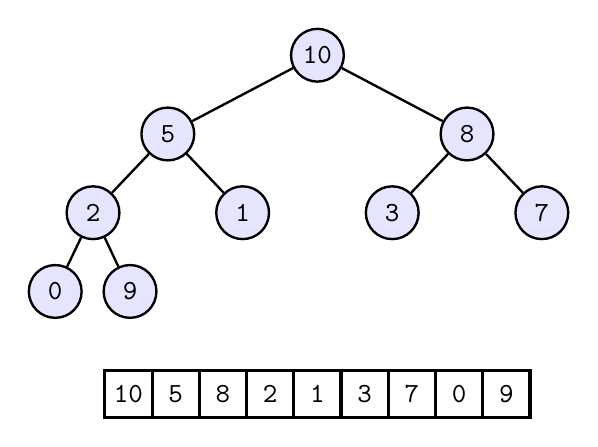
\begin{tikzpicture}

\fill[blue!10] (0.0, 0.0) circle (0.35);
\node [line width=0.03cm,black,minimum size=0.6699999999999999cm,draw,circle] at (0.0,0.0)(10){};\draw (0.0, 0.0) node[color=black] {\texttt{10}};
\fill[blue!10] (-1.9, -1.0) circle (0.35);
\node [line width=0.03cm,black,minimum size=0.6699999999999999cm,draw,circle] at (-1.9,-1.0)(5){};\draw (-1.9, -1.0) node[color=black] {\texttt{5}};
\fill[blue!10] (1.9, -1.0) circle (0.35);
\node [line width=0.03cm,black,minimum size=0.6699999999999999cm,draw,circle] at (1.9,-1.0)(8){};\draw (1.9, -1.0) node[color=black] {\texttt{8}};
\fill[blue!10] (-2.85, -2.0) circle (0.35);
\node [line width=0.03cm,black,minimum size=0.6699999999999999cm,draw,circle] at (-2.85,-2.0)(2){};\draw (-2.85, -2.0) node[color=black] {\texttt{2}};
\fill[blue!10] (-0.95, -2.0) circle (0.35);
\node [line width=0.03cm,black,minimum size=0.6699999999999999cm,draw,circle] at (-0.95,-2.0)(1){};\draw (-0.95, -2.0) node[color=black] {\texttt{1}};
\fill[blue!10] (0.95, -2.0) circle (0.35);
\node [line width=0.03cm,black,minimum size=0.6699999999999999cm,draw,circle] at (0.95,-2.0)(3){};\draw (0.95, -2.0) node[color=black] {\texttt{3}};
\fill[blue!10] (2.85, -2.0) circle (0.35);
\node [line width=0.03cm,black,minimum size=0.6699999999999999cm,draw,circle] at (2.85,-2.0)(7){};\draw (2.85, -2.0) node[color=black] {\texttt{7}};
\fill[blue!10] (-3.33, -3.0) circle (0.35);
\node [line width=0.03cm,black,minimum size=0.6699999999999999cm,draw,circle] at (-3.33,-3.0)(0){};\draw (-3.33, -3.0) node[color=black] {\texttt{0}};
\fill[blue!10] (-2.38, -3.0) circle (0.35);
\node [line width=0.03cm,black,minimum size=0.6699999999999999cm,draw,circle] at (-2.38,-3.0)(9){};\draw (-2.38, -3.0) node[color=black] {\texttt{9}};\draw[line width=0.03cm,black] (10) to  (5);
\draw[line width=0.03cm,black] (10) to  (8);
\draw[line width=0.03cm,black] (5) to  (2);
\draw[line width=0.03cm,black] (5) to  (1);
\draw[line width=0.03cm,black] (8) to  (3);
\draw[line width=0.03cm,black] (8) to  (7);
\draw[line width=0.03cm,black] (2) to  (0);
\draw[line width=0.03cm,black] (2) to  (9);

\draw (-2.3999999999999995, -4.299999999999999)
  node[draw, line width=0.04cm, , color=black,
       rounded corners=0cm, inner sep=0cm] {

\begin{minipage}[t][0.6cm]{0.6cm}
\mbox{}

\end{minipage}

};\draw (-2.3999999999999995, -4.299999999999999) node[color=black] {{\texttt{10}}};
\draw (-1.7999999999999996, -4.299999999999999)
  node[draw, line width=0.04cm, , color=black,
       rounded corners=0cm, inner sep=0cm] {

\begin{minipage}[t][0.6cm]{0.6cm}
\mbox{}

\end{minipage}

};\draw (-1.7999999999999996, -4.299999999999999) node[color=black] {{\texttt{5}}};
\draw (-1.1999999999999997, -4.299999999999999)
  node[draw, line width=0.04cm, , color=black,
       rounded corners=0cm, inner sep=0cm] {

\begin{minipage}[t][0.6cm]{0.6cm}
\mbox{}

\end{minipage}

};\draw (-1.1999999999999997, -4.299999999999999) node[color=black] {{\texttt{8}}};
\draw (-0.5999999999999996, -4.299999999999999)
  node[draw, line width=0.04cm, , color=black,
       rounded corners=0cm, inner sep=0cm] {

\begin{minipage}[t][0.6cm]{0.6cm}
\mbox{}

\end{minipage}

};\draw (-0.5999999999999996, -4.299999999999999) node[color=black] {{\texttt{2}}};
\draw (4.440892098500626e-16, -4.299999999999999)
  node[draw, line width=0.04cm, , color=black,
       rounded corners=0cm, inner sep=0cm] {

\begin{minipage}[t][0.6cm]{0.6cm}
\mbox{}

\end{minipage}

};\draw (4.440892098500626e-16, -4.299999999999999) node[color=black] {{\texttt{1}}};
\draw (0.6000000000000005, -4.299999999999999)
  node[draw, line width=0.04cm, , color=black,
       rounded corners=0cm, inner sep=0cm] {

\begin{minipage}[t][0.6cm]{0.6cm}
\mbox{}

\end{minipage}

};\draw (0.6000000000000005, -4.299999999999999) node[color=black] {{\texttt{3}}};
\draw (1.2000000000000006, -4.299999999999999)
  node[draw, line width=0.04cm, , color=black,
       rounded corners=0cm, inner sep=0cm] {

\begin{minipage}[t][0.6cm]{0.6cm}
\mbox{}

\end{minipage}

};\draw (1.2000000000000006, -4.299999999999999) node[color=black] {{\texttt{7}}};
\draw (1.8000000000000007, -4.299999999999999)
  node[draw, line width=0.04cm, , color=black,
       rounded corners=0cm, inner sep=0cm] {

\begin{minipage}[t][0.6cm]{0.6cm}
\mbox{}

\end{minipage}

};\draw (1.8000000000000007, -4.299999999999999) node[color=black] {{\texttt{0}}};
\draw (2.4000000000000004, -4.299999999999999)
  node[draw, line width=0.04cm, , color=black,
       rounded corners=0cm, inner sep=0cm] {

\begin{minipage}[t][0.6cm]{0.6cm}
\mbox{}

\end{minipage}

};\draw (2.4000000000000004, -4.299999999999999) node[color=black] {{\texttt{9}}};
\end{tikzpicture}

\end{center}



Notice that while working on the entry at $(3,1)$, we looked at 
$(1,1),(2,2)$ and also $(2,1),(1,3)$.
Do you notice that there's a pattern in the pairs of cells that
contribute to the two cases in filling the cell at $(3,1)$?
%-*-latex-*-

\begin{center}
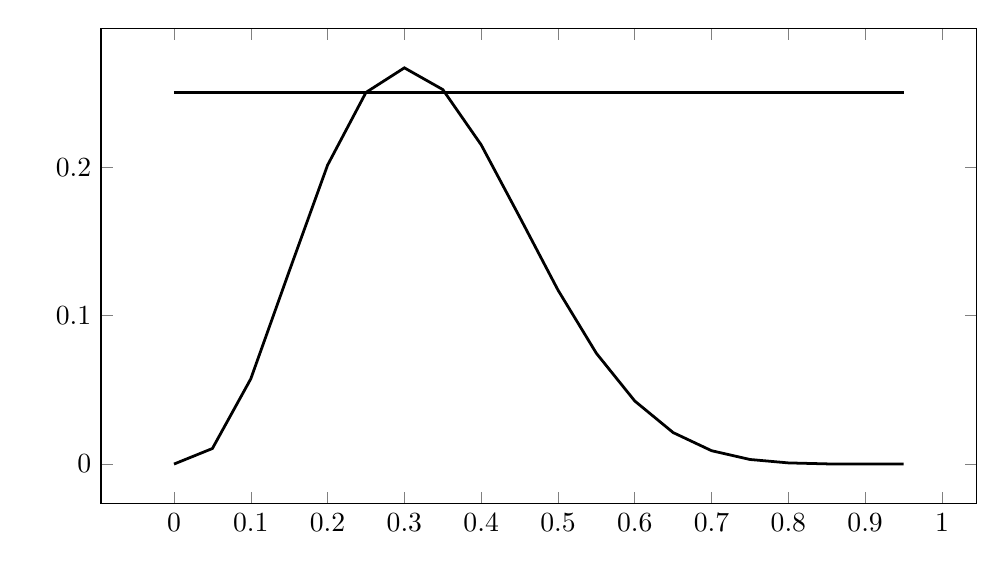
\begin{tikzpicture}[line width=1]
\begin{axis}[width=5in, height=3in,
             scatter/classes={a={mark=*,draw=black}},
             xlabel={\mbox{}},
             xlabel style={name=xlabel}, 
             ylabel={\mbox{}}, 
             legend style={
                at={(xlabel.south)},
                yshift=-1ex,
                anchor=north,
                legend cell align=left,
                },
        ]
]
\addplot[draw=black, line width=1] coordinates {(0.0, 0.0)
(0.05, 0.010475059441406248)
(0.1, 0.05739562800000002)
(0.15, 0.1298337207539062)
(0.2, 0.2013265920000001)
(0.25, 0.25028228759765625)
(0.3, 0.2668279319999998)
(0.35, 0.25221962497265626)
(0.4, 0.21499084799999998)
(0.45, 0.1664782928789064)
(0.5, 0.1171875)
(0.55, 0.07460310631640622)
(0.6, 0.042467328000000006)
(0.65, 0.02120301528515624)
(0.7, 0.009001692000000007)
(0.75, 0.00308990478515625)
(0.8, 0.000786431999999999)
(0.85, 0.0001259148164062501)
(0.9, 8.747999999999988e-06)
(0.95, 8.037890625000049e-08)};\addplot[draw=black, line width=1] coordinates {(0.0, 0.25)
(0.05, 0.25)
(0.1, 0.25)
(0.15, 0.25)
(0.2, 0.25)
(0.25, 0.25)
(0.3, 0.25)
(0.35, 0.25)
(0.4, 0.25)
(0.45, 0.25)
(0.5, 0.25)
(0.55, 0.25)
(0.6, 0.25)
(0.65, 0.25)
(0.7, 0.25)
(0.75, 0.25)
(0.8, 0.25)
(0.85, 0.25)
(0.9, 0.25)
(0.95, 0.25)};
\end{axis}\end{tikzpicture}\end{center}


Now we move on the the entry at $(3,2)$:
%-*-latex-*-

\begin{center}
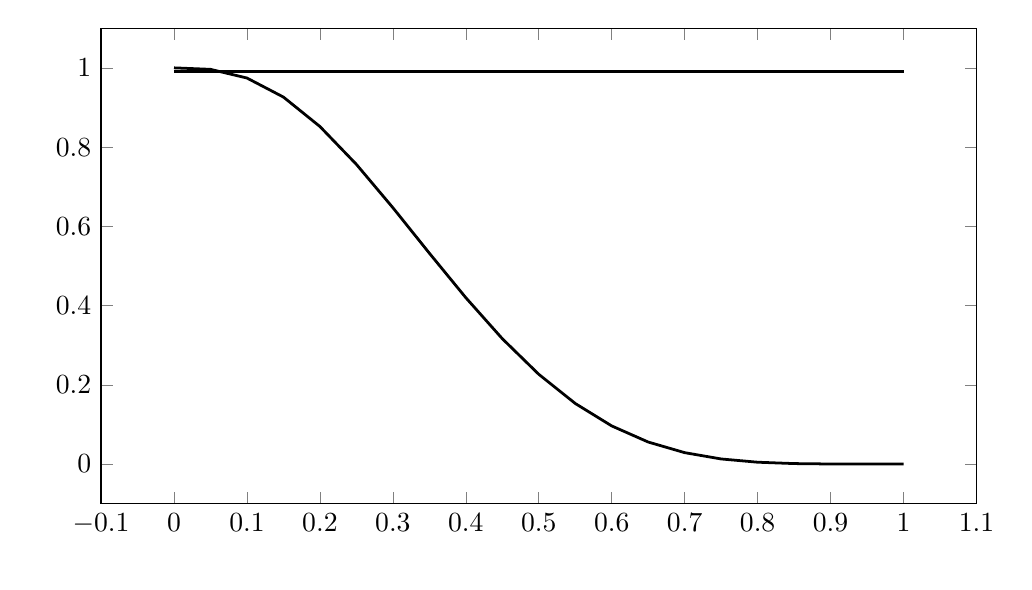
\begin{tikzpicture}[line width=1]
\begin{axis}[width=5in, height=3in,
             scatter/classes={a={mark=*,draw=black}},
             xlabel={\mbox{}},
             xlabel style={name=xlabel}, 
             ylabel={\mbox{}}, 
             legend style={
                at={(xlabel.south)},
                yshift=-1ex,
                anchor=north,
                legend cell align=left,
                },
        ]
]
\addplot[draw=black, line width=1] coordinates {(0.0, 1.0)
(0.05, 0.9962429570312497)
(0.1, 0.9743085000000002)
(0.15, 0.9262348398437498)
(0.2, 0.8519680000000004)
(0.25, 0.75640869140625)
(0.3, 0.6470694999999997)
(0.35, 0.53228332421875)
(0.4, 0.41990399999999994)
(0.45, 0.31644005078125015)
(0.5, 0.2265625)
(0.55, 0.15292768359374995)
(0.6, 0.09625600000000004)
(0.65, 0.055607535156249985)
(0.7, 0.02879550000000002)
(0.75, 0.01287841796875)
(0.8, 0.004671999999999996)
(0.85, 0.0012216445312500006)
(0.9, 0.00017649999999999982)
(0.95, 6.0273437500000275e-06)
(1.0, 0.0)};\addplot[draw=black, line width=1] coordinates {(0.0, 0.99)
(0.05, 0.99)
(0.1, 0.99)
(0.15, 0.99)
(0.2, 0.99)
(0.25, 0.99)
(0.3, 0.99)
(0.35, 0.99)
(0.4, 0.99)
(0.45, 0.99)
(0.5, 0.99)
(0.55, 0.99)
(0.6, 0.99)
(0.65, 0.99)
(0.7, 0.99)
(0.75, 0.99)
(0.8, 0.99)
(0.85, 0.99)
(0.9, 0.99)
(0.95, 0.99)
(1.0, 0.99)};
\end{axis}\end{tikzpicture}\end{center}


This corresponds to $w_{2,3}$ and
\[
w_{2,3} = w_{2,1}w_{3,2} \hskip 1cm \text{or} \hskip 1cm w_{2,2}w_{4,1}
\] 
First for $w_{2,3} = w_{2,1}w_{3,2}$, we want to find variables that can derive
$AC$; there's only one: $S$.
\begin{center}
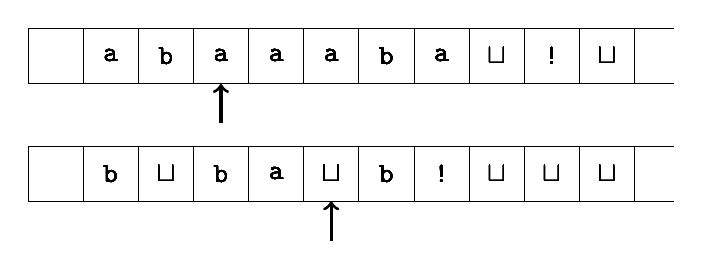
\begin{tikzpicture}

\draw (0.35, 0.35)
  node[draw, line width=0.01cm, , color=black,
       rounded corners=0cm, inner sep=0cm] {

\begin{minipage}[t][0.7cm]{0.7cm}
\mbox{}

\end{minipage}

};\draw (0.35, 0.35) node[color=black] {\texttt{\DOLLAR}};
\draw (1.0499999999999998, 0.35)
  node[draw, line width=0.01cm, , color=black,
       rounded corners=0cm, inner sep=0cm] {

\begin{minipage}[t][0.7cm]{0.7cm}
\mbox{}

\end{minipage}

};\draw (1.0499999999999998, 0.35) node[color=black] {\texttt{a}};
\draw (1.7499999999999998, 0.35)
  node[draw, line width=0.01cm, , color=black,
       rounded corners=0cm, inner sep=0cm] {

\begin{minipage}[t][0.7cm]{0.7cm}
\mbox{}

\end{minipage}

};\draw (1.7499999999999998, 0.35) node[color=black] {\texttt{b}};
\draw (2.4499999999999997, 0.35)
  node[draw, line width=0.01cm, , color=black,
       rounded corners=0cm, inner sep=0cm] {

\begin{minipage}[t][0.7cm]{0.7cm}
\mbox{}

\end{minipage}

};\draw (2.4499999999999997, 0.35) node[color=black] {\texttt{a}};
\draw (3.15, 0.35)
  node[draw, line width=0.01cm, , color=black,
       rounded corners=0cm, inner sep=0cm] {

\begin{minipage}[t][0.7cm]{0.7cm}
\mbox{}

\end{minipage}

};\draw (3.15, 0.35) node[color=black] {\texttt{a}};
\draw (3.85, 0.35)
  node[draw, line width=0.01cm, , color=black,
       rounded corners=0cm, inner sep=0cm] {

\begin{minipage}[t][0.7cm]{0.7cm}
\mbox{}

\end{minipage}

};\draw (3.85, 0.35) node[color=black] {\texttt{a}};
\draw (4.550000000000001, 0.35)
  node[draw, line width=0.01cm, , color=black,
       rounded corners=0cm, inner sep=0cm] {

\begin{minipage}[t][0.7cm]{0.7cm}
\mbox{}

\end{minipage}

};\draw (4.550000000000001, 0.35) node[color=black] {\texttt{b}};
\draw (5.25, 0.35)
  node[draw, line width=0.01cm, , color=black,
       rounded corners=0cm, inner sep=0cm] {

\begin{minipage}[t][0.7cm]{0.7cm}
\mbox{}

\end{minipage}

};\draw (5.25, 0.35) node[color=black] {\texttt{a}};
\draw (5.950000000000001, 0.35)
  node[draw, line width=0.01cm, , color=black,
       rounded corners=0cm, inner sep=0cm] {

\begin{minipage}[t][0.7cm]{0.7cm}
\mbox{}

\end{minipage}

};\draw (5.950000000000001, 0.35) node[color=black] {\texttt{$\sqcup$}};
\draw (6.65, 0.35)
  node[draw, line width=0.01cm, , color=black,
       rounded corners=0cm, inner sep=0cm] {

\begin{minipage}[t][0.7cm]{0.7cm}
\mbox{}

\end{minipage}

};\draw (6.65, 0.35) node[color=black] {\texttt{!}};
\draw (7.350000000000001, 0.35)
  node[draw, line width=0.01cm, , color=black,
       rounded corners=0cm, inner sep=0cm] {

\begin{minipage}[t][0.7cm]{0.7cm}
\mbox{}

\end{minipage}

};\draw (7.350000000000001, 0.35) node[color=black] {\texttt{$\sqcup$}};
\draw (0.35, 0.35)
  node[draw, line width=0.01cm, , color=black,
       rounded corners=0cm, inner sep=0cm] {

\begin{minipage}[t][0.7cm]{0.7cm}
\mbox{}

\end{minipage}

};\draw (0.35, 0.35) node[color=black] {\texttt{\DOLLAR}};
\draw (1.0499999999999998, 0.35)
  node[draw, line width=0.01cm, , color=black,
       rounded corners=0cm, inner sep=0cm] {

\begin{minipage}[t][0.7cm]{0.7cm}
\mbox{}

\end{minipage}

};\draw (1.0499999999999998, 0.35) node[color=black] {\texttt{a}};
\draw (1.7499999999999998, 0.35)
  node[draw, line width=0.01cm, , color=black,
       rounded corners=0cm, inner sep=0cm] {

\begin{minipage}[t][0.7cm]{0.7cm}
\mbox{}

\end{minipage}

};\draw (1.7499999999999998, 0.35) node[color=black] {\texttt{b}};
\draw (2.4499999999999997, 0.35)
  node[draw, line width=0.01cm, , color=black,
       rounded corners=0cm, inner sep=0cm] {

\begin{minipage}[t][0.7cm]{0.7cm}
\mbox{}

\end{minipage}

};\draw (2.4499999999999997, 0.35) node[color=black] {\texttt{a}};
\draw (3.15, 0.35)
  node[draw, line width=0.01cm, , color=black,
       rounded corners=0cm, inner sep=0cm] {

\begin{minipage}[t][0.7cm]{0.7cm}
\mbox{}

\end{minipage}

};\draw (3.15, 0.35) node[color=black] {\texttt{a}};
\draw (3.85, 0.35)
  node[draw, line width=0.01cm, , color=black,
       rounded corners=0cm, inner sep=0cm] {

\begin{minipage}[t][0.7cm]{0.7cm}
\mbox{}

\end{minipage}

};\draw (3.85, 0.35) node[color=black] {\texttt{a}};
\draw (4.550000000000001, 0.35)
  node[draw, line width=0.01cm, , color=black,
       rounded corners=0cm, inner sep=0cm] {

\begin{minipage}[t][0.7cm]{0.7cm}
\mbox{}

\end{minipage}

};\draw (4.550000000000001, 0.35) node[color=black] {\texttt{b}};
\draw (5.25, 0.35)
  node[draw, line width=0.01cm, , color=black,
       rounded corners=0cm, inner sep=0cm] {

\begin{minipage}[t][0.7cm]{0.7cm}
\mbox{}

\end{minipage}

};\draw (5.25, 0.35) node[color=black] {\texttt{a}};
\draw (5.950000000000001, 0.35)
  node[draw, line width=0.01cm, , color=black,
       rounded corners=0cm, inner sep=0cm] {

\begin{minipage}[t][0.7cm]{0.7cm}
\mbox{}

\end{minipage}

};\draw (5.950000000000001, 0.35) node[color=black] {\texttt{$\sqcup$}};
\draw (6.65, 0.35)
  node[draw, line width=0.01cm, , color=black,
       rounded corners=0cm, inner sep=0cm] {

\begin{minipage}[t][0.7cm]{0.7cm}
\mbox{}

\end{minipage}

};\draw (6.65, 0.35) node[color=black] {\texttt{!}};
\draw (7.350000000000001, 0.35)
  node[draw, line width=0.01cm, , color=black,
       rounded corners=0cm, inner sep=0cm] {

\begin{minipage}[t][0.7cm]{0.7cm}
\mbox{}

\end{minipage}

};\draw (7.350000000000001, 0.35) node[color=black] {\texttt{$\sqcup$}};
\draw (0.35, 0.35)
  node[draw, line width=0.01cm, , color=black,
       rounded corners=0cm, inner sep=0cm] {

\begin{minipage}[t][0.7cm]{0.7cm}
\mbox{}

\end{minipage}

};\draw (0.35, 0.35) node[color=black] {\texttt{\DOLLAR}};
\draw (1.0499999999999998, 0.35)
  node[draw, line width=0.01cm, , color=black,
       rounded corners=0cm, inner sep=0cm] {

\begin{minipage}[t][0.7cm]{0.7cm}
\mbox{}

\end{minipage}

};\draw (1.0499999999999998, 0.35) node[color=black] {\texttt{a}};
\draw (1.7499999999999998, 0.35)
  node[draw, line width=0.01cm, , color=black,
       rounded corners=0cm, inner sep=0cm] {

\begin{minipage}[t][0.7cm]{0.7cm}
\mbox{}

\end{minipage}

};\draw (1.7499999999999998, 0.35) node[color=black] {\texttt{b}};
\draw (2.4499999999999997, 0.35)
  node[draw, line width=0.01cm, , color=black,
       rounded corners=0cm, inner sep=0cm] {

\begin{minipage}[t][0.7cm]{0.7cm}
\mbox{}

\end{minipage}

};\draw (2.4499999999999997, 0.35) node[color=black] {\texttt{a}};
\draw (3.15, 0.35)
  node[draw, line width=0.01cm, , color=black,
       rounded corners=0cm, inner sep=0cm] {

\begin{minipage}[t][0.7cm]{0.7cm}
\mbox{}

\end{minipage}

};\draw (3.15, 0.35) node[color=black] {\texttt{a}};
\draw (3.85, 0.35)
  node[draw, line width=0.01cm, , color=black,
       rounded corners=0cm, inner sep=0cm] {

\begin{minipage}[t][0.7cm]{0.7cm}
\mbox{}

\end{minipage}

};\draw (3.85, 0.35) node[color=black] {\texttt{a}};
\draw (4.550000000000001, 0.35)
  node[draw, line width=0.01cm, , color=black,
       rounded corners=0cm, inner sep=0cm] {

\begin{minipage}[t][0.7cm]{0.7cm}
\mbox{}

\end{minipage}

};\draw (4.550000000000001, 0.35) node[color=black] {\texttt{b}};
\draw (5.25, 0.35)
  node[draw, line width=0.01cm, , color=black,
       rounded corners=0cm, inner sep=0cm] {

\begin{minipage}[t][0.7cm]{0.7cm}
\mbox{}

\end{minipage}

};\draw (5.25, 0.35) node[color=black] {\texttt{a}};
\draw (5.950000000000001, 0.35)
  node[draw, line width=0.01cm, , color=black,
       rounded corners=0cm, inner sep=0cm] {

\begin{minipage}[t][0.7cm]{0.7cm}
\mbox{}

\end{minipage}

};\draw (5.950000000000001, 0.35) node[color=black] {\texttt{$\sqcup$}};
\draw (6.65, 0.35)
  node[draw, line width=0.01cm, , color=black,
       rounded corners=0cm, inner sep=0cm] {

\begin{minipage}[t][0.7cm]{0.7cm}
\mbox{}

\end{minipage}

};\draw (6.65, 0.35) node[color=black] {\texttt{!}};
\draw (7.350000000000001, 0.35)
  node[draw, line width=0.01cm, , color=black,
       rounded corners=0cm, inner sep=0cm] {

\begin{minipage}[t][0.7cm]{0.7cm}
\mbox{}

\end{minipage}

};\draw (7.350000000000001, 0.35) node[color=black] {\texttt{$\sqcup$}};
\draw (0.35, 0.35)
  node[draw, line width=0.01cm, , color=black,
       rounded corners=0cm, inner sep=0cm] {

\begin{minipage}[t][0.7cm]{0.7cm}
\mbox{}

\end{minipage}

};\draw (0.35, 0.35) node[color=black] {\texttt{\DOLLAR}};
\draw (1.0499999999999998, 0.35)
  node[draw, line width=0.01cm, , color=black,
       rounded corners=0cm, inner sep=0cm] {

\begin{minipage}[t][0.7cm]{0.7cm}
\mbox{}

\end{minipage}

};\draw (1.0499999999999998, 0.35) node[color=black] {\texttt{a}};
\draw (1.7499999999999998, 0.35)
  node[draw, line width=0.01cm, , color=black,
       rounded corners=0cm, inner sep=0cm] {

\begin{minipage}[t][0.7cm]{0.7cm}
\mbox{}

\end{minipage}

};\draw (1.7499999999999998, 0.35) node[color=black] {\texttt{b}};
\draw (2.4499999999999997, 0.35)
  node[draw, line width=0.01cm, , color=black,
       rounded corners=0cm, inner sep=0cm] {

\begin{minipage}[t][0.7cm]{0.7cm}
\mbox{}

\end{minipage}

};\draw (2.4499999999999997, 0.35) node[color=black] {\texttt{a}};
\draw (3.15, 0.35)
  node[draw, line width=0.01cm, , color=black,
       rounded corners=0cm, inner sep=0cm] {

\begin{minipage}[t][0.7cm]{0.7cm}
\mbox{}

\end{minipage}

};\draw (3.15, 0.35) node[color=black] {\texttt{a}};
\draw (3.85, 0.35)
  node[draw, line width=0.01cm, , color=black,
       rounded corners=0cm, inner sep=0cm] {

\begin{minipage}[t][0.7cm]{0.7cm}
\mbox{}

\end{minipage}

};\draw (3.85, 0.35) node[color=black] {\texttt{a}};
\draw (4.550000000000001, 0.35)
  node[draw, line width=0.01cm, , color=black,
       rounded corners=0cm, inner sep=0cm] {

\begin{minipage}[t][0.7cm]{0.7cm}
\mbox{}

\end{minipage}

};\draw (4.550000000000001, 0.35) node[color=black] {\texttt{b}};
\draw (5.25, 0.35)
  node[draw, line width=0.01cm, , color=black,
       rounded corners=0cm, inner sep=0cm] {

\begin{minipage}[t][0.7cm]{0.7cm}
\mbox{}

\end{minipage}

};\draw (5.25, 0.35) node[color=black] {\texttt{a}};
\draw (5.950000000000001, 0.35)
  node[draw, line width=0.01cm, , color=black,
       rounded corners=0cm, inner sep=0cm] {

\begin{minipage}[t][0.7cm]{0.7cm}
\mbox{}

\end{minipage}

};\draw (5.950000000000001, 0.35) node[color=black] {\texttt{$\sqcup$}};
\draw (6.65, 0.35)
  node[draw, line width=0.01cm, , color=black,
       rounded corners=0cm, inner sep=0cm] {

\begin{minipage}[t][0.7cm]{0.7cm}
\mbox{}

\end{minipage}

};\draw (6.65, 0.35) node[color=black] {\texttt{!}};
\draw (7.350000000000001, 0.35)
  node[draw, line width=0.01cm, , color=black,
       rounded corners=0cm, inner sep=0cm] {

\begin{minipage}[t][0.7cm]{0.7cm}
\mbox{}

\end{minipage}

};\draw (7.350000000000001, 0.35) node[color=black] {\texttt{$\sqcup$}};
\draw (0.35, 0.35)
  node[draw, line width=0.01cm, , color=black,
       rounded corners=0cm, inner sep=0cm] {

\begin{minipage}[t][0.7cm]{0.7cm}
\mbox{}

\end{minipage}

};\draw (0.35, 0.35) node[color=black] {\texttt{\DOLLAR}};
\draw (1.0499999999999998, 0.35)
  node[draw, line width=0.01cm, , color=black,
       rounded corners=0cm, inner sep=0cm] {

\begin{minipage}[t][0.7cm]{0.7cm}
\mbox{}

\end{minipage}

};\draw (1.0499999999999998, 0.35) node[color=black] {\texttt{a}};
\draw (1.7499999999999998, 0.35)
  node[draw, line width=0.01cm, , color=black,
       rounded corners=0cm, inner sep=0cm] {

\begin{minipage}[t][0.7cm]{0.7cm}
\mbox{}

\end{minipage}

};\draw (1.7499999999999998, 0.35) node[color=black] {\texttt{b}};
\draw (2.4499999999999997, 0.35)
  node[draw, line width=0.01cm, , color=black,
       rounded corners=0cm, inner sep=0cm] {

\begin{minipage}[t][0.7cm]{0.7cm}
\mbox{}

\end{minipage}

};\draw (2.4499999999999997, 0.35) node[color=black] {\texttt{a}};
\draw (3.15, 0.35)
  node[draw, line width=0.01cm, , color=black,
       rounded corners=0cm, inner sep=0cm] {

\begin{minipage}[t][0.7cm]{0.7cm}
\mbox{}

\end{minipage}

};\draw (3.15, 0.35) node[color=black] {\texttt{a}};
\draw (3.85, 0.35)
  node[draw, line width=0.01cm, , color=black,
       rounded corners=0cm, inner sep=0cm] {

\begin{minipage}[t][0.7cm]{0.7cm}
\mbox{}

\end{minipage}

};\draw (3.85, 0.35) node[color=black] {\texttt{a}};
\draw (4.550000000000001, 0.35)
  node[draw, line width=0.01cm, , color=black,
       rounded corners=0cm, inner sep=0cm] {

\begin{minipage}[t][0.7cm]{0.7cm}
\mbox{}

\end{minipage}

};\draw (4.550000000000001, 0.35) node[color=black] {\texttt{b}};
\draw (5.25, 0.35)
  node[draw, line width=0.01cm, , color=black,
       rounded corners=0cm, inner sep=0cm] {

\begin{minipage}[t][0.7cm]{0.7cm}
\mbox{}

\end{minipage}

};\draw (5.25, 0.35) node[color=black] {\texttt{a}};
\draw (5.950000000000001, 0.35)
  node[draw, line width=0.01cm, , color=black,
       rounded corners=0cm, inner sep=0cm] {

\begin{minipage}[t][0.7cm]{0.7cm}
\mbox{}

\end{minipage}

};\draw (5.950000000000001, 0.35) node[color=black] {\texttt{$\sqcup$}};
\draw (6.65, 0.35)
  node[draw, line width=0.01cm, , color=black,
       rounded corners=0cm, inner sep=0cm] {

\begin{minipage}[t][0.7cm]{0.7cm}
\mbox{}

\end{minipage}

};\draw (6.65, 0.35) node[color=black] {\texttt{!}};
\draw (7.350000000000001, 0.35)
  node[draw, line width=0.01cm, , color=black,
       rounded corners=0cm, inner sep=0cm] {

\begin{minipage}[t][0.7cm]{0.7cm}
\mbox{}

\end{minipage}

};\draw (7.350000000000001, 0.35) node[color=black] {\texttt{$\sqcup$}};
\draw (0.35, 0.35)
  node[draw, line width=0.01cm, , color=black,
       rounded corners=0cm, inner sep=0cm] {

\begin{minipage}[t][0.7cm]{0.7cm}
\mbox{}

\end{minipage}

};\draw (0.35, 0.35) node[color=black] {\texttt{\DOLLAR}};
\draw (1.0499999999999998, 0.35)
  node[draw, line width=0.01cm, , color=black,
       rounded corners=0cm, inner sep=0cm] {

\begin{minipage}[t][0.7cm]{0.7cm}
\mbox{}

\end{minipage}

};\draw (1.0499999999999998, 0.35) node[color=black] {\texttt{a}};
\draw (1.7499999999999998, 0.35)
  node[draw, line width=0.01cm, , color=black,
       rounded corners=0cm, inner sep=0cm] {

\begin{minipage}[t][0.7cm]{0.7cm}
\mbox{}

\end{minipage}

};\draw (1.7499999999999998, 0.35) node[color=black] {\texttt{b}};
\draw (2.4499999999999997, 0.35)
  node[draw, line width=0.01cm, , color=black,
       rounded corners=0cm, inner sep=0cm] {

\begin{minipage}[t][0.7cm]{0.7cm}
\mbox{}

\end{minipage}

};\draw (2.4499999999999997, 0.35) node[color=black] {\texttt{a}};
\draw (3.15, 0.35)
  node[draw, line width=0.01cm, , color=black,
       rounded corners=0cm, inner sep=0cm] {

\begin{minipage}[t][0.7cm]{0.7cm}
\mbox{}

\end{minipage}

};\draw (3.15, 0.35) node[color=black] {\texttt{a}};
\draw (3.85, 0.35)
  node[draw, line width=0.01cm, , color=black,
       rounded corners=0cm, inner sep=0cm] {

\begin{minipage}[t][0.7cm]{0.7cm}
\mbox{}

\end{minipage}

};\draw (3.85, 0.35) node[color=black] {\texttt{a}};
\draw (4.550000000000001, 0.35)
  node[draw, line width=0.01cm, , color=black,
       rounded corners=0cm, inner sep=0cm] {

\begin{minipage}[t][0.7cm]{0.7cm}
\mbox{}

\end{minipage}

};\draw (4.550000000000001, 0.35) node[color=black] {\texttt{b}};
\draw (5.25, 0.35)
  node[draw, line width=0.01cm, , color=black,
       rounded corners=0cm, inner sep=0cm] {

\begin{minipage}[t][0.7cm]{0.7cm}
\mbox{}

\end{minipage}

};\draw (5.25, 0.35) node[color=black] {\texttt{a}};
\draw (5.950000000000001, 0.35)
  node[draw, line width=0.01cm, , color=black,
       rounded corners=0cm, inner sep=0cm] {

\begin{minipage}[t][0.7cm]{0.7cm}
\mbox{}

\end{minipage}

};\draw (5.950000000000001, 0.35) node[color=black] {\texttt{$\sqcup$}};
\draw (6.65, 0.35)
  node[draw, line width=0.01cm, , color=black,
       rounded corners=0cm, inner sep=0cm] {

\begin{minipage}[t][0.7cm]{0.7cm}
\mbox{}

\end{minipage}

};\draw (6.65, 0.35) node[color=black] {\texttt{!}};
\draw (7.350000000000001, 0.35)
  node[draw, line width=0.01cm, , color=black,
       rounded corners=0cm, inner sep=0cm] {

\begin{minipage}[t][0.7cm]{0.7cm}
\mbox{}

\end{minipage}

};\draw (7.350000000000001, 0.35) node[color=black] {\texttt{$\sqcup$}};
\draw (0.35, 0.35)
  node[draw, line width=0.01cm, , color=black,
       rounded corners=0cm, inner sep=0cm] {

\begin{minipage}[t][0.7cm]{0.7cm}
\mbox{}

\end{minipage}

};\draw (0.35, 0.35) node[color=black] {\texttt{\DOLLAR}};
\draw (1.0499999999999998, 0.35)
  node[draw, line width=0.01cm, , color=black,
       rounded corners=0cm, inner sep=0cm] {

\begin{minipage}[t][0.7cm]{0.7cm}
\mbox{}

\end{minipage}

};\draw (1.0499999999999998, 0.35) node[color=black] {\texttt{a}};
\draw (1.7499999999999998, 0.35)
  node[draw, line width=0.01cm, , color=black,
       rounded corners=0cm, inner sep=0cm] {

\begin{minipage}[t][0.7cm]{0.7cm}
\mbox{}

\end{minipage}

};\draw (1.7499999999999998, 0.35) node[color=black] {\texttt{b}};
\draw (2.4499999999999997, 0.35)
  node[draw, line width=0.01cm, , color=black,
       rounded corners=0cm, inner sep=0cm] {

\begin{minipage}[t][0.7cm]{0.7cm}
\mbox{}

\end{minipage}

};\draw (2.4499999999999997, 0.35) node[color=black] {\texttt{a}};
\draw (3.15, 0.35)
  node[draw, line width=0.01cm, , color=black,
       rounded corners=0cm, inner sep=0cm] {

\begin{minipage}[t][0.7cm]{0.7cm}
\mbox{}

\end{minipage}

};\draw (3.15, 0.35) node[color=black] {\texttt{a}};
\draw (3.85, 0.35)
  node[draw, line width=0.01cm, , color=black,
       rounded corners=0cm, inner sep=0cm] {

\begin{minipage}[t][0.7cm]{0.7cm}
\mbox{}

\end{minipage}

};\draw (3.85, 0.35) node[color=black] {\texttt{a}};
\draw (4.550000000000001, 0.35)
  node[draw, line width=0.01cm, , color=black,
       rounded corners=0cm, inner sep=0cm] {

\begin{minipage}[t][0.7cm]{0.7cm}
\mbox{}

\end{minipage}

};\draw (4.550000000000001, 0.35) node[color=black] {\texttt{b}};
\draw (5.25, 0.35)
  node[draw, line width=0.01cm, , color=black,
       rounded corners=0cm, inner sep=0cm] {

\begin{minipage}[t][0.7cm]{0.7cm}
\mbox{}

\end{minipage}

};\draw (5.25, 0.35) node[color=black] {\texttt{a}};
\draw (5.950000000000001, 0.35)
  node[draw, line width=0.01cm, , color=black,
       rounded corners=0cm, inner sep=0cm] {

\begin{minipage}[t][0.7cm]{0.7cm}
\mbox{}

\end{minipage}

};\draw (5.950000000000001, 0.35) node[color=black] {\texttt{$\sqcup$}};
\draw (6.65, 0.35)
  node[draw, line width=0.01cm, , color=black,
       rounded corners=0cm, inner sep=0cm] {

\begin{minipage}[t][0.7cm]{0.7cm}
\mbox{}

\end{minipage}

};\draw (6.65, 0.35) node[color=black] {\texttt{!}};
\draw (7.350000000000001, 0.35)
  node[draw, line width=0.01cm, , color=black,
       rounded corners=0cm, inner sep=0cm] {

\begin{minipage}[t][0.7cm]{0.7cm}
\mbox{}

\end{minipage}

};\draw (7.350000000000001, 0.35) node[color=black] {\texttt{$\sqcup$}};
\draw (0.35, 0.35)
  node[draw, line width=0.01cm, , color=black,
       rounded corners=0cm, inner sep=0cm] {

\begin{minipage}[t][0.7cm]{0.7cm}
\mbox{}

\end{minipage}

};\draw (0.35, 0.35) node[color=black] {\texttt{\DOLLAR}};
\draw (1.0499999999999998, 0.35)
  node[draw, line width=0.01cm, , color=black,
       rounded corners=0cm, inner sep=0cm] {

\begin{minipage}[t][0.7cm]{0.7cm}
\mbox{}

\end{minipage}

};\draw (1.0499999999999998, 0.35) node[color=black] {\texttt{a}};
\draw (1.7499999999999998, 0.35)
  node[draw, line width=0.01cm, , color=black,
       rounded corners=0cm, inner sep=0cm] {

\begin{minipage}[t][0.7cm]{0.7cm}
\mbox{}

\end{minipage}

};\draw (1.7499999999999998, 0.35) node[color=black] {\texttt{b}};
\draw (2.4499999999999997, 0.35)
  node[draw, line width=0.01cm, , color=black,
       rounded corners=0cm, inner sep=0cm] {

\begin{minipage}[t][0.7cm]{0.7cm}
\mbox{}

\end{minipage}

};\draw (2.4499999999999997, 0.35) node[color=black] {\texttt{a}};
\draw (3.15, 0.35)
  node[draw, line width=0.01cm, , color=black,
       rounded corners=0cm, inner sep=0cm] {

\begin{minipage}[t][0.7cm]{0.7cm}
\mbox{}

\end{minipage}

};\draw (3.15, 0.35) node[color=black] {\texttt{a}};
\draw (3.85, 0.35)
  node[draw, line width=0.01cm, , color=black,
       rounded corners=0cm, inner sep=0cm] {

\begin{minipage}[t][0.7cm]{0.7cm}
\mbox{}

\end{minipage}

};\draw (3.85, 0.35) node[color=black] {\texttt{a}};
\draw (4.550000000000001, 0.35)
  node[draw, line width=0.01cm, , color=black,
       rounded corners=0cm, inner sep=0cm] {

\begin{minipage}[t][0.7cm]{0.7cm}
\mbox{}

\end{minipage}

};\draw (4.550000000000001, 0.35) node[color=black] {\texttt{b}};
\draw (5.25, 0.35)
  node[draw, line width=0.01cm, , color=black,
       rounded corners=0cm, inner sep=0cm] {

\begin{minipage}[t][0.7cm]{0.7cm}
\mbox{}

\end{minipage}

};\draw (5.25, 0.35) node[color=black] {\texttt{a}};
\draw (5.950000000000001, 0.35)
  node[draw, line width=0.01cm, , color=black,
       rounded corners=0cm, inner sep=0cm] {

\begin{minipage}[t][0.7cm]{0.7cm}
\mbox{}

\end{minipage}

};\draw (5.950000000000001, 0.35) node[color=black] {\texttt{$\sqcup$}};
\draw (6.65, 0.35)
  node[draw, line width=0.01cm, , color=black,
       rounded corners=0cm, inner sep=0cm] {

\begin{minipage}[t][0.7cm]{0.7cm}
\mbox{}

\end{minipage}

};\draw (6.65, 0.35) node[color=black] {\texttt{!}};
\draw (7.350000000000001, 0.35)
  node[draw, line width=0.01cm, , color=black,
       rounded corners=0cm, inner sep=0cm] {

\begin{minipage}[t][0.7cm]{0.7cm}
\mbox{}

\end{minipage}

};\draw (7.350000000000001, 0.35) node[color=black] {\texttt{$\sqcup$}};
\draw (0.35, 0.35)
  node[draw, line width=0.01cm, , color=black,
       rounded corners=0cm, inner sep=0cm] {

\begin{minipage}[t][0.7cm]{0.7cm}
\mbox{}

\end{minipage}

};\draw (0.35, 0.35) node[color=black] {\texttt{\DOLLAR}};
\draw (1.0499999999999998, 0.35)
  node[draw, line width=0.01cm, , color=black,
       rounded corners=0cm, inner sep=0cm] {

\begin{minipage}[t][0.7cm]{0.7cm}
\mbox{}

\end{minipage}

};\draw (1.0499999999999998, 0.35) node[color=black] {\texttt{a}};
\draw (1.7499999999999998, 0.35)
  node[draw, line width=0.01cm, , color=black,
       rounded corners=0cm, inner sep=0cm] {

\begin{minipage}[t][0.7cm]{0.7cm}
\mbox{}

\end{minipage}

};\draw (1.7499999999999998, 0.35) node[color=black] {\texttt{b}};
\draw (2.4499999999999997, 0.35)
  node[draw, line width=0.01cm, , color=black,
       rounded corners=0cm, inner sep=0cm] {

\begin{minipage}[t][0.7cm]{0.7cm}
\mbox{}

\end{minipage}

};\draw (2.4499999999999997, 0.35) node[color=black] {\texttt{a}};
\draw (3.15, 0.35)
  node[draw, line width=0.01cm, , color=black,
       rounded corners=0cm, inner sep=0cm] {

\begin{minipage}[t][0.7cm]{0.7cm}
\mbox{}

\end{minipage}

};\draw (3.15, 0.35) node[color=black] {\texttt{a}};
\draw (3.85, 0.35)
  node[draw, line width=0.01cm, , color=black,
       rounded corners=0cm, inner sep=0cm] {

\begin{minipage}[t][0.7cm]{0.7cm}
\mbox{}

\end{minipage}

};\draw (3.85, 0.35) node[color=black] {\texttt{a}};
\draw (4.550000000000001, 0.35)
  node[draw, line width=0.01cm, , color=black,
       rounded corners=0cm, inner sep=0cm] {

\begin{minipage}[t][0.7cm]{0.7cm}
\mbox{}

\end{minipage}

};\draw (4.550000000000001, 0.35) node[color=black] {\texttt{b}};
\draw (5.25, 0.35)
  node[draw, line width=0.01cm, , color=black,
       rounded corners=0cm, inner sep=0cm] {

\begin{minipage}[t][0.7cm]{0.7cm}
\mbox{}

\end{minipage}

};\draw (5.25, 0.35) node[color=black] {\texttt{a}};
\draw (5.950000000000001, 0.35)
  node[draw, line width=0.01cm, , color=black,
       rounded corners=0cm, inner sep=0cm] {

\begin{minipage}[t][0.7cm]{0.7cm}
\mbox{}

\end{minipage}

};\draw (5.950000000000001, 0.35) node[color=black] {\texttt{$\sqcup$}};
\draw (6.65, 0.35)
  node[draw, line width=0.01cm, , color=black,
       rounded corners=0cm, inner sep=0cm] {

\begin{minipage}[t][0.7cm]{0.7cm}
\mbox{}

\end{minipage}

};\draw (6.65, 0.35) node[color=black] {\texttt{!}};
\draw (7.350000000000001, 0.35)
  node[draw, line width=0.01cm, , color=black,
       rounded corners=0cm, inner sep=0cm] {

\begin{minipage}[t][0.7cm]{0.7cm}
\mbox{}

\end{minipage}

};\draw (7.350000000000001, 0.35) node[color=black] {\texttt{$\sqcup$}};
\draw (0.35, 0.35)
  node[draw, line width=0.01cm, , color=black,
       rounded corners=0cm, inner sep=0cm] {

\begin{minipage}[t][0.7cm]{0.7cm}
\mbox{}

\end{minipage}

};\draw (0.35, 0.35) node[color=black] {\texttt{\DOLLAR}};
\draw (1.0499999999999998, 0.35)
  node[draw, line width=0.01cm, , color=black,
       rounded corners=0cm, inner sep=0cm] {

\begin{minipage}[t][0.7cm]{0.7cm}
\mbox{}

\end{minipage}

};\draw (1.0499999999999998, 0.35) node[color=black] {\texttt{a}};
\draw (1.7499999999999998, 0.35)
  node[draw, line width=0.01cm, , color=black,
       rounded corners=0cm, inner sep=0cm] {

\begin{minipage}[t][0.7cm]{0.7cm}
\mbox{}

\end{minipage}

};\draw (1.7499999999999998, 0.35) node[color=black] {\texttt{b}};
\draw (2.4499999999999997, 0.35)
  node[draw, line width=0.01cm, , color=black,
       rounded corners=0cm, inner sep=0cm] {

\begin{minipage}[t][0.7cm]{0.7cm}
\mbox{}

\end{minipage}

};\draw (2.4499999999999997, 0.35) node[color=black] {\texttt{a}};
\draw (3.15, 0.35)
  node[draw, line width=0.01cm, , color=black,
       rounded corners=0cm, inner sep=0cm] {

\begin{minipage}[t][0.7cm]{0.7cm}
\mbox{}

\end{minipage}

};\draw (3.15, 0.35) node[color=black] {\texttt{a}};
\draw (3.85, 0.35)
  node[draw, line width=0.01cm, , color=black,
       rounded corners=0cm, inner sep=0cm] {

\begin{minipage}[t][0.7cm]{0.7cm}
\mbox{}

\end{minipage}

};\draw (3.85, 0.35) node[color=black] {\texttt{a}};
\draw (4.550000000000001, 0.35)
  node[draw, line width=0.01cm, , color=black,
       rounded corners=0cm, inner sep=0cm] {

\begin{minipage}[t][0.7cm]{0.7cm}
\mbox{}

\end{minipage}

};\draw (4.550000000000001, 0.35) node[color=black] {\texttt{b}};
\draw (5.25, 0.35)
  node[draw, line width=0.01cm, , color=black,
       rounded corners=0cm, inner sep=0cm] {

\begin{minipage}[t][0.7cm]{0.7cm}
\mbox{}

\end{minipage}

};\draw (5.25, 0.35) node[color=black] {\texttt{a}};
\draw (5.950000000000001, 0.35)
  node[draw, line width=0.01cm, , color=black,
       rounded corners=0cm, inner sep=0cm] {

\begin{minipage}[t][0.7cm]{0.7cm}
\mbox{}

\end{minipage}

};\draw (5.950000000000001, 0.35) node[color=black] {\texttt{$\sqcup$}};
\draw (6.65, 0.35)
  node[draw, line width=0.01cm, , color=black,
       rounded corners=0cm, inner sep=0cm] {

\begin{minipage}[t][0.7cm]{0.7cm}
\mbox{}

\end{minipage}

};\draw (6.65, 0.35) node[color=black] {\texttt{!}};
\draw (7.350000000000001, 0.35)
  node[draw, line width=0.01cm, , color=black,
       rounded corners=0cm, inner sep=0cm] {

\begin{minipage}[t][0.7cm]{0.7cm}
\mbox{}

\end{minipage}

};\draw (7.350000000000001, 0.35) node[color=black] {\texttt{$\sqcup$}};
\draw (0.35, 0.35)
  node[draw, line width=0.01cm, , color=black,
       rounded corners=0cm, inner sep=0cm] {

\begin{minipage}[t][0.7cm]{0.7cm}
\mbox{}

\end{minipage}

};\draw (0.35, 0.35) node[color=black] {\texttt{\DOLLAR}};
\draw (1.0499999999999998, 0.35)
  node[draw, line width=0.01cm, , color=black,
       rounded corners=0cm, inner sep=0cm] {

\begin{minipage}[t][0.7cm]{0.7cm}
\mbox{}

\end{minipage}

};\draw (1.0499999999999998, 0.35) node[color=black] {\texttt{a}};
\draw (1.7499999999999998, 0.35)
  node[draw, line width=0.01cm, , color=black,
       rounded corners=0cm, inner sep=0cm] {

\begin{minipage}[t][0.7cm]{0.7cm}
\mbox{}

\end{minipage}

};\draw (1.7499999999999998, 0.35) node[color=black] {\texttt{b}};
\draw (2.4499999999999997, 0.35)
  node[draw, line width=0.01cm, , color=black,
       rounded corners=0cm, inner sep=0cm] {

\begin{minipage}[t][0.7cm]{0.7cm}
\mbox{}

\end{minipage}

};\draw (2.4499999999999997, 0.35) node[color=black] {\texttt{a}};
\draw (3.15, 0.35)
  node[draw, line width=0.01cm, , color=black,
       rounded corners=0cm, inner sep=0cm] {

\begin{minipage}[t][0.7cm]{0.7cm}
\mbox{}

\end{minipage}

};\draw (3.15, 0.35) node[color=black] {\texttt{a}};
\draw (3.85, 0.35)
  node[draw, line width=0.01cm, , color=black,
       rounded corners=0cm, inner sep=0cm] {

\begin{minipage}[t][0.7cm]{0.7cm}
\mbox{}

\end{minipage}

};\draw (3.85, 0.35) node[color=black] {\texttt{a}};
\draw (4.550000000000001, 0.35)
  node[draw, line width=0.01cm, , color=black,
       rounded corners=0cm, inner sep=0cm] {

\begin{minipage}[t][0.7cm]{0.7cm}
\mbox{}

\end{minipage}

};\draw (4.550000000000001, 0.35) node[color=black] {\texttt{b}};
\draw (5.25, 0.35)
  node[draw, line width=0.01cm, , color=black,
       rounded corners=0cm, inner sep=0cm] {

\begin{minipage}[t][0.7cm]{0.7cm}
\mbox{}

\end{minipage}

};\draw (5.25, 0.35) node[color=black] {\texttt{a}};
\draw (5.950000000000001, 0.35)
  node[draw, line width=0.01cm, , color=black,
       rounded corners=0cm, inner sep=0cm] {

\begin{minipage}[t][0.7cm]{0.7cm}
\mbox{}

\end{minipage}

};\draw (5.950000000000001, 0.35) node[color=black] {\texttt{$\sqcup$}};
\draw (6.65, 0.35)
  node[draw, line width=0.01cm, , color=black,
       rounded corners=0cm, inner sep=0cm] {

\begin{minipage}[t][0.7cm]{0.7cm}
\mbox{}

\end{minipage}

};\draw (6.65, 0.35) node[color=black] {\texttt{!}};
\draw (7.350000000000001, 0.35)
  node[draw, line width=0.01cm, , color=black,
       rounded corners=0cm, inner sep=0cm] {

\begin{minipage}[t][0.7cm]{0.7cm}
\mbox{}

\end{minipage}

};\draw (7.350000000000001, 0.35) node[color=black] {\texttt{$\sqcup$}};\draw[line width=0.01cm,black] (7.700000000000001,0.7) to  (8.200000000000001,0.7);
\draw[line width=0.01cm,black] (7.700000000000001,0.0) to  (8.200000000000001,0.0);
\draw[line width=0.04cm,black,->] (2.45,-0.51) to  (2.45,-0.01);

\draw (0.35, -1.15)
  node[draw, line width=0.01cm, , color=black,
       rounded corners=0cm, inner sep=0cm] {

\begin{minipage}[t][0.7cm]{0.7cm}
\mbox{}

\end{minipage}

};\draw (0.35, -1.15) node[color=black] {\texttt{\DOLLAR}};
\draw (1.0499999999999998, -1.15)
  node[draw, line width=0.01cm, , color=black,
       rounded corners=0cm, inner sep=0cm] {

\begin{minipage}[t][0.7cm]{0.7cm}
\mbox{}

\end{minipage}

};\draw (1.0499999999999998, -1.15) node[color=black] {\texttt{b}};
\draw (1.7499999999999998, -1.15)
  node[draw, line width=0.01cm, , color=black,
       rounded corners=0cm, inner sep=0cm] {

\begin{minipage}[t][0.7cm]{0.7cm}
\mbox{}

\end{minipage}

};\draw (1.7499999999999998, -1.15) node[color=black] {\texttt{$\sqcup$}};
\draw (2.4499999999999997, -1.15)
  node[draw, line width=0.01cm, , color=black,
       rounded corners=0cm, inner sep=0cm] {

\begin{minipage}[t][0.7cm]{0.7cm}
\mbox{}

\end{minipage}

};\draw (2.4499999999999997, -1.15) node[color=black] {\texttt{b}};
\draw (3.15, -1.15)
  node[draw, line width=0.01cm, , color=black,
       rounded corners=0cm, inner sep=0cm] {

\begin{minipage}[t][0.7cm]{0.7cm}
\mbox{}

\end{minipage}

};\draw (3.15, -1.15) node[color=black] {\texttt{a}};
\draw (3.85, -1.15)
  node[draw, line width=0.01cm, , color=black,
       rounded corners=0cm, inner sep=0cm] {

\begin{minipage}[t][0.7cm]{0.7cm}
\mbox{}

\end{minipage}

};\draw (3.85, -1.15) node[color=black] {\texttt{$\sqcup$}};
\draw (4.550000000000001, -1.15)
  node[draw, line width=0.01cm, , color=black,
       rounded corners=0cm, inner sep=0cm] {

\begin{minipage}[t][0.7cm]{0.7cm}
\mbox{}

\end{minipage}

};\draw (4.550000000000001, -1.15) node[color=black] {\texttt{b}};
\draw (5.25, -1.15)
  node[draw, line width=0.01cm, , color=black,
       rounded corners=0cm, inner sep=0cm] {

\begin{minipage}[t][0.7cm]{0.7cm}
\mbox{}

\end{minipage}

};\draw (5.25, -1.15) node[color=black] {\texttt{!}};
\draw (5.950000000000001, -1.15)
  node[draw, line width=0.01cm, , color=black,
       rounded corners=0cm, inner sep=0cm] {

\begin{minipage}[t][0.7cm]{0.7cm}
\mbox{}

\end{minipage}

};\draw (5.950000000000001, -1.15) node[color=black] {\texttt{$\sqcup$}};
\draw (6.65, -1.15)
  node[draw, line width=0.01cm, , color=black,
       rounded corners=0cm, inner sep=0cm] {

\begin{minipage}[t][0.7cm]{0.7cm}
\mbox{}

\end{minipage}

};\draw (6.65, -1.15) node[color=black] {\texttt{$\sqcup$}};
\draw (7.350000000000001, -1.15)
  node[draw, line width=0.01cm, , color=black,
       rounded corners=0cm, inner sep=0cm] {

\begin{minipage}[t][0.7cm]{0.7cm}
\mbox{}

\end{minipage}

};\draw (7.350000000000001, -1.15) node[color=black] {\texttt{$\sqcup$}};
\draw (0.35, -1.15)
  node[draw, line width=0.01cm, , color=black,
       rounded corners=0cm, inner sep=0cm] {

\begin{minipage}[t][0.7cm]{0.7cm}
\mbox{}

\end{minipage}

};\draw (0.35, -1.15) node[color=black] {\texttt{\DOLLAR}};
\draw (1.0499999999999998, -1.15)
  node[draw, line width=0.01cm, , color=black,
       rounded corners=0cm, inner sep=0cm] {

\begin{minipage}[t][0.7cm]{0.7cm}
\mbox{}

\end{minipage}

};\draw (1.0499999999999998, -1.15) node[color=black] {\texttt{b}};
\draw (1.7499999999999998, -1.15)
  node[draw, line width=0.01cm, , color=black,
       rounded corners=0cm, inner sep=0cm] {

\begin{minipage}[t][0.7cm]{0.7cm}
\mbox{}

\end{minipage}

};\draw (1.7499999999999998, -1.15) node[color=black] {\texttt{$\sqcup$}};
\draw (2.4499999999999997, -1.15)
  node[draw, line width=0.01cm, , color=black,
       rounded corners=0cm, inner sep=0cm] {

\begin{minipage}[t][0.7cm]{0.7cm}
\mbox{}

\end{minipage}

};\draw (2.4499999999999997, -1.15) node[color=black] {\texttt{b}};
\draw (3.15, -1.15)
  node[draw, line width=0.01cm, , color=black,
       rounded corners=0cm, inner sep=0cm] {

\begin{minipage}[t][0.7cm]{0.7cm}
\mbox{}

\end{minipage}

};\draw (3.15, -1.15) node[color=black] {\texttt{a}};
\draw (3.85, -1.15)
  node[draw, line width=0.01cm, , color=black,
       rounded corners=0cm, inner sep=0cm] {

\begin{minipage}[t][0.7cm]{0.7cm}
\mbox{}

\end{minipage}

};\draw (3.85, -1.15) node[color=black] {\texttt{$\sqcup$}};
\draw (4.550000000000001, -1.15)
  node[draw, line width=0.01cm, , color=black,
       rounded corners=0cm, inner sep=0cm] {

\begin{minipage}[t][0.7cm]{0.7cm}
\mbox{}

\end{minipage}

};\draw (4.550000000000001, -1.15) node[color=black] {\texttt{b}};
\draw (5.25, -1.15)
  node[draw, line width=0.01cm, , color=black,
       rounded corners=0cm, inner sep=0cm] {

\begin{minipage}[t][0.7cm]{0.7cm}
\mbox{}

\end{minipage}

};\draw (5.25, -1.15) node[color=black] {\texttt{!}};
\draw (5.950000000000001, -1.15)
  node[draw, line width=0.01cm, , color=black,
       rounded corners=0cm, inner sep=0cm] {

\begin{minipage}[t][0.7cm]{0.7cm}
\mbox{}

\end{minipage}

};\draw (5.950000000000001, -1.15) node[color=black] {\texttt{$\sqcup$}};
\draw (6.65, -1.15)
  node[draw, line width=0.01cm, , color=black,
       rounded corners=0cm, inner sep=0cm] {

\begin{minipage}[t][0.7cm]{0.7cm}
\mbox{}

\end{minipage}

};\draw (6.65, -1.15) node[color=black] {\texttt{$\sqcup$}};
\draw (7.350000000000001, -1.15)
  node[draw, line width=0.01cm, , color=black,
       rounded corners=0cm, inner sep=0cm] {

\begin{minipage}[t][0.7cm]{0.7cm}
\mbox{}

\end{minipage}

};\draw (7.350000000000001, -1.15) node[color=black] {\texttt{$\sqcup$}};
\draw (0.35, -1.15)
  node[draw, line width=0.01cm, , color=black,
       rounded corners=0cm, inner sep=0cm] {

\begin{minipage}[t][0.7cm]{0.7cm}
\mbox{}

\end{minipage}

};\draw (0.35, -1.15) node[color=black] {\texttt{\DOLLAR}};
\draw (1.0499999999999998, -1.15)
  node[draw, line width=0.01cm, , color=black,
       rounded corners=0cm, inner sep=0cm] {

\begin{minipage}[t][0.7cm]{0.7cm}
\mbox{}

\end{minipage}

};\draw (1.0499999999999998, -1.15) node[color=black] {\texttt{b}};
\draw (1.7499999999999998, -1.15)
  node[draw, line width=0.01cm, , color=black,
       rounded corners=0cm, inner sep=0cm] {

\begin{minipage}[t][0.7cm]{0.7cm}
\mbox{}

\end{minipage}

};\draw (1.7499999999999998, -1.15) node[color=black] {\texttt{$\sqcup$}};
\draw (2.4499999999999997, -1.15)
  node[draw, line width=0.01cm, , color=black,
       rounded corners=0cm, inner sep=0cm] {

\begin{minipage}[t][0.7cm]{0.7cm}
\mbox{}

\end{minipage}

};\draw (2.4499999999999997, -1.15) node[color=black] {\texttt{b}};
\draw (3.15, -1.15)
  node[draw, line width=0.01cm, , color=black,
       rounded corners=0cm, inner sep=0cm] {

\begin{minipage}[t][0.7cm]{0.7cm}
\mbox{}

\end{minipage}

};\draw (3.15, -1.15) node[color=black] {\texttt{a}};
\draw (3.85, -1.15)
  node[draw, line width=0.01cm, , color=black,
       rounded corners=0cm, inner sep=0cm] {

\begin{minipage}[t][0.7cm]{0.7cm}
\mbox{}

\end{minipage}

};\draw (3.85, -1.15) node[color=black] {\texttt{$\sqcup$}};
\draw (4.550000000000001, -1.15)
  node[draw, line width=0.01cm, , color=black,
       rounded corners=0cm, inner sep=0cm] {

\begin{minipage}[t][0.7cm]{0.7cm}
\mbox{}

\end{minipage}

};\draw (4.550000000000001, -1.15) node[color=black] {\texttt{b}};
\draw (5.25, -1.15)
  node[draw, line width=0.01cm, , color=black,
       rounded corners=0cm, inner sep=0cm] {

\begin{minipage}[t][0.7cm]{0.7cm}
\mbox{}

\end{minipage}

};\draw (5.25, -1.15) node[color=black] {\texttt{!}};
\draw (5.950000000000001, -1.15)
  node[draw, line width=0.01cm, , color=black,
       rounded corners=0cm, inner sep=0cm] {

\begin{minipage}[t][0.7cm]{0.7cm}
\mbox{}

\end{minipage}

};\draw (5.950000000000001, -1.15) node[color=black] {\texttt{$\sqcup$}};
\draw (6.65, -1.15)
  node[draw, line width=0.01cm, , color=black,
       rounded corners=0cm, inner sep=0cm] {

\begin{minipage}[t][0.7cm]{0.7cm}
\mbox{}

\end{minipage}

};\draw (6.65, -1.15) node[color=black] {\texttt{$\sqcup$}};
\draw (7.350000000000001, -1.15)
  node[draw, line width=0.01cm, , color=black,
       rounded corners=0cm, inner sep=0cm] {

\begin{minipage}[t][0.7cm]{0.7cm}
\mbox{}

\end{minipage}

};\draw (7.350000000000001, -1.15) node[color=black] {\texttt{$\sqcup$}};
\draw (0.35, -1.15)
  node[draw, line width=0.01cm, , color=black,
       rounded corners=0cm, inner sep=0cm] {

\begin{minipage}[t][0.7cm]{0.7cm}
\mbox{}

\end{minipage}

};\draw (0.35, -1.15) node[color=black] {\texttt{\DOLLAR}};
\draw (1.0499999999999998, -1.15)
  node[draw, line width=0.01cm, , color=black,
       rounded corners=0cm, inner sep=0cm] {

\begin{minipage}[t][0.7cm]{0.7cm}
\mbox{}

\end{minipage}

};\draw (1.0499999999999998, -1.15) node[color=black] {\texttt{b}};
\draw (1.7499999999999998, -1.15)
  node[draw, line width=0.01cm, , color=black,
       rounded corners=0cm, inner sep=0cm] {

\begin{minipage}[t][0.7cm]{0.7cm}
\mbox{}

\end{minipage}

};\draw (1.7499999999999998, -1.15) node[color=black] {\texttt{$\sqcup$}};
\draw (2.4499999999999997, -1.15)
  node[draw, line width=0.01cm, , color=black,
       rounded corners=0cm, inner sep=0cm] {

\begin{minipage}[t][0.7cm]{0.7cm}
\mbox{}

\end{minipage}

};\draw (2.4499999999999997, -1.15) node[color=black] {\texttt{b}};
\draw (3.15, -1.15)
  node[draw, line width=0.01cm, , color=black,
       rounded corners=0cm, inner sep=0cm] {

\begin{minipage}[t][0.7cm]{0.7cm}
\mbox{}

\end{minipage}

};\draw (3.15, -1.15) node[color=black] {\texttt{a}};
\draw (3.85, -1.15)
  node[draw, line width=0.01cm, , color=black,
       rounded corners=0cm, inner sep=0cm] {

\begin{minipage}[t][0.7cm]{0.7cm}
\mbox{}

\end{minipage}

};\draw (3.85, -1.15) node[color=black] {\texttt{$\sqcup$}};
\draw (4.550000000000001, -1.15)
  node[draw, line width=0.01cm, , color=black,
       rounded corners=0cm, inner sep=0cm] {

\begin{minipage}[t][0.7cm]{0.7cm}
\mbox{}

\end{minipage}

};\draw (4.550000000000001, -1.15) node[color=black] {\texttt{b}};
\draw (5.25, -1.15)
  node[draw, line width=0.01cm, , color=black,
       rounded corners=0cm, inner sep=0cm] {

\begin{minipage}[t][0.7cm]{0.7cm}
\mbox{}

\end{minipage}

};\draw (5.25, -1.15) node[color=black] {\texttt{!}};
\draw (5.950000000000001, -1.15)
  node[draw, line width=0.01cm, , color=black,
       rounded corners=0cm, inner sep=0cm] {

\begin{minipage}[t][0.7cm]{0.7cm}
\mbox{}

\end{minipage}

};\draw (5.950000000000001, -1.15) node[color=black] {\texttt{$\sqcup$}};
\draw (6.65, -1.15)
  node[draw, line width=0.01cm, , color=black,
       rounded corners=0cm, inner sep=0cm] {

\begin{minipage}[t][0.7cm]{0.7cm}
\mbox{}

\end{minipage}

};\draw (6.65, -1.15) node[color=black] {\texttt{$\sqcup$}};
\draw (7.350000000000001, -1.15)
  node[draw, line width=0.01cm, , color=black,
       rounded corners=0cm, inner sep=0cm] {

\begin{minipage}[t][0.7cm]{0.7cm}
\mbox{}

\end{minipage}

};\draw (7.350000000000001, -1.15) node[color=black] {\texttt{$\sqcup$}};
\draw (0.35, -1.15)
  node[draw, line width=0.01cm, , color=black,
       rounded corners=0cm, inner sep=0cm] {

\begin{minipage}[t][0.7cm]{0.7cm}
\mbox{}

\end{minipage}

};\draw (0.35, -1.15) node[color=black] {\texttt{\DOLLAR}};
\draw (1.0499999999999998, -1.15)
  node[draw, line width=0.01cm, , color=black,
       rounded corners=0cm, inner sep=0cm] {

\begin{minipage}[t][0.7cm]{0.7cm}
\mbox{}

\end{minipage}

};\draw (1.0499999999999998, -1.15) node[color=black] {\texttt{b}};
\draw (1.7499999999999998, -1.15)
  node[draw, line width=0.01cm, , color=black,
       rounded corners=0cm, inner sep=0cm] {

\begin{minipage}[t][0.7cm]{0.7cm}
\mbox{}

\end{minipage}

};\draw (1.7499999999999998, -1.15) node[color=black] {\texttt{$\sqcup$}};
\draw (2.4499999999999997, -1.15)
  node[draw, line width=0.01cm, , color=black,
       rounded corners=0cm, inner sep=0cm] {

\begin{minipage}[t][0.7cm]{0.7cm}
\mbox{}

\end{minipage}

};\draw (2.4499999999999997, -1.15) node[color=black] {\texttt{b}};
\draw (3.15, -1.15)
  node[draw, line width=0.01cm, , color=black,
       rounded corners=0cm, inner sep=0cm] {

\begin{minipage}[t][0.7cm]{0.7cm}
\mbox{}

\end{minipage}

};\draw (3.15, -1.15) node[color=black] {\texttt{a}};
\draw (3.85, -1.15)
  node[draw, line width=0.01cm, , color=black,
       rounded corners=0cm, inner sep=0cm] {

\begin{minipage}[t][0.7cm]{0.7cm}
\mbox{}

\end{minipage}

};\draw (3.85, -1.15) node[color=black] {\texttt{$\sqcup$}};
\draw (4.550000000000001, -1.15)
  node[draw, line width=0.01cm, , color=black,
       rounded corners=0cm, inner sep=0cm] {

\begin{minipage}[t][0.7cm]{0.7cm}
\mbox{}

\end{minipage}

};\draw (4.550000000000001, -1.15) node[color=black] {\texttt{b}};
\draw (5.25, -1.15)
  node[draw, line width=0.01cm, , color=black,
       rounded corners=0cm, inner sep=0cm] {

\begin{minipage}[t][0.7cm]{0.7cm}
\mbox{}

\end{minipage}

};\draw (5.25, -1.15) node[color=black] {\texttt{!}};
\draw (5.950000000000001, -1.15)
  node[draw, line width=0.01cm, , color=black,
       rounded corners=0cm, inner sep=0cm] {

\begin{minipage}[t][0.7cm]{0.7cm}
\mbox{}

\end{minipage}

};\draw (5.950000000000001, -1.15) node[color=black] {\texttt{$\sqcup$}};
\draw (6.65, -1.15)
  node[draw, line width=0.01cm, , color=black,
       rounded corners=0cm, inner sep=0cm] {

\begin{minipage}[t][0.7cm]{0.7cm}
\mbox{}

\end{minipage}

};\draw (6.65, -1.15) node[color=black] {\texttt{$\sqcup$}};
\draw (7.350000000000001, -1.15)
  node[draw, line width=0.01cm, , color=black,
       rounded corners=0cm, inner sep=0cm] {

\begin{minipage}[t][0.7cm]{0.7cm}
\mbox{}

\end{minipage}

};\draw (7.350000000000001, -1.15) node[color=black] {\texttt{$\sqcup$}};
\draw (0.35, -1.15)
  node[draw, line width=0.01cm, , color=black,
       rounded corners=0cm, inner sep=0cm] {

\begin{minipage}[t][0.7cm]{0.7cm}
\mbox{}

\end{minipage}

};\draw (0.35, -1.15) node[color=black] {\texttt{\DOLLAR}};
\draw (1.0499999999999998, -1.15)
  node[draw, line width=0.01cm, , color=black,
       rounded corners=0cm, inner sep=0cm] {

\begin{minipage}[t][0.7cm]{0.7cm}
\mbox{}

\end{minipage}

};\draw (1.0499999999999998, -1.15) node[color=black] {\texttt{b}};
\draw (1.7499999999999998, -1.15)
  node[draw, line width=0.01cm, , color=black,
       rounded corners=0cm, inner sep=0cm] {

\begin{minipage}[t][0.7cm]{0.7cm}
\mbox{}

\end{minipage}

};\draw (1.7499999999999998, -1.15) node[color=black] {\texttt{$\sqcup$}};
\draw (2.4499999999999997, -1.15)
  node[draw, line width=0.01cm, , color=black,
       rounded corners=0cm, inner sep=0cm] {

\begin{minipage}[t][0.7cm]{0.7cm}
\mbox{}

\end{minipage}

};\draw (2.4499999999999997, -1.15) node[color=black] {\texttt{b}};
\draw (3.15, -1.15)
  node[draw, line width=0.01cm, , color=black,
       rounded corners=0cm, inner sep=0cm] {

\begin{minipage}[t][0.7cm]{0.7cm}
\mbox{}

\end{minipage}

};\draw (3.15, -1.15) node[color=black] {\texttt{a}};
\draw (3.85, -1.15)
  node[draw, line width=0.01cm, , color=black,
       rounded corners=0cm, inner sep=0cm] {

\begin{minipage}[t][0.7cm]{0.7cm}
\mbox{}

\end{minipage}

};\draw (3.85, -1.15) node[color=black] {\texttt{$\sqcup$}};
\draw (4.550000000000001, -1.15)
  node[draw, line width=0.01cm, , color=black,
       rounded corners=0cm, inner sep=0cm] {

\begin{minipage}[t][0.7cm]{0.7cm}
\mbox{}

\end{minipage}

};\draw (4.550000000000001, -1.15) node[color=black] {\texttt{b}};
\draw (5.25, -1.15)
  node[draw, line width=0.01cm, , color=black,
       rounded corners=0cm, inner sep=0cm] {

\begin{minipage}[t][0.7cm]{0.7cm}
\mbox{}

\end{minipage}

};\draw (5.25, -1.15) node[color=black] {\texttt{!}};
\draw (5.950000000000001, -1.15)
  node[draw, line width=0.01cm, , color=black,
       rounded corners=0cm, inner sep=0cm] {

\begin{minipage}[t][0.7cm]{0.7cm}
\mbox{}

\end{minipage}

};\draw (5.950000000000001, -1.15) node[color=black] {\texttt{$\sqcup$}};
\draw (6.65, -1.15)
  node[draw, line width=0.01cm, , color=black,
       rounded corners=0cm, inner sep=0cm] {

\begin{minipage}[t][0.7cm]{0.7cm}
\mbox{}

\end{minipage}

};\draw (6.65, -1.15) node[color=black] {\texttt{$\sqcup$}};
\draw (7.350000000000001, -1.15)
  node[draw, line width=0.01cm, , color=black,
       rounded corners=0cm, inner sep=0cm] {

\begin{minipage}[t][0.7cm]{0.7cm}
\mbox{}

\end{minipage}

};\draw (7.350000000000001, -1.15) node[color=black] {\texttt{$\sqcup$}};
\draw (0.35, -1.15)
  node[draw, line width=0.01cm, , color=black,
       rounded corners=0cm, inner sep=0cm] {

\begin{minipage}[t][0.7cm]{0.7cm}
\mbox{}

\end{minipage}

};\draw (0.35, -1.15) node[color=black] {\texttt{\DOLLAR}};
\draw (1.0499999999999998, -1.15)
  node[draw, line width=0.01cm, , color=black,
       rounded corners=0cm, inner sep=0cm] {

\begin{minipage}[t][0.7cm]{0.7cm}
\mbox{}

\end{minipage}

};\draw (1.0499999999999998, -1.15) node[color=black] {\texttt{b}};
\draw (1.7499999999999998, -1.15)
  node[draw, line width=0.01cm, , color=black,
       rounded corners=0cm, inner sep=0cm] {

\begin{minipage}[t][0.7cm]{0.7cm}
\mbox{}

\end{minipage}

};\draw (1.7499999999999998, -1.15) node[color=black] {\texttt{$\sqcup$}};
\draw (2.4499999999999997, -1.15)
  node[draw, line width=0.01cm, , color=black,
       rounded corners=0cm, inner sep=0cm] {

\begin{minipage}[t][0.7cm]{0.7cm}
\mbox{}

\end{minipage}

};\draw (2.4499999999999997, -1.15) node[color=black] {\texttt{b}};
\draw (3.15, -1.15)
  node[draw, line width=0.01cm, , color=black,
       rounded corners=0cm, inner sep=0cm] {

\begin{minipage}[t][0.7cm]{0.7cm}
\mbox{}

\end{minipage}

};\draw (3.15, -1.15) node[color=black] {\texttt{a}};
\draw (3.85, -1.15)
  node[draw, line width=0.01cm, , color=black,
       rounded corners=0cm, inner sep=0cm] {

\begin{minipage}[t][0.7cm]{0.7cm}
\mbox{}

\end{minipage}

};\draw (3.85, -1.15) node[color=black] {\texttt{$\sqcup$}};
\draw (4.550000000000001, -1.15)
  node[draw, line width=0.01cm, , color=black,
       rounded corners=0cm, inner sep=0cm] {

\begin{minipage}[t][0.7cm]{0.7cm}
\mbox{}

\end{minipage}

};\draw (4.550000000000001, -1.15) node[color=black] {\texttt{b}};
\draw (5.25, -1.15)
  node[draw, line width=0.01cm, , color=black,
       rounded corners=0cm, inner sep=0cm] {

\begin{minipage}[t][0.7cm]{0.7cm}
\mbox{}

\end{minipage}

};\draw (5.25, -1.15) node[color=black] {\texttt{!}};
\draw (5.950000000000001, -1.15)
  node[draw, line width=0.01cm, , color=black,
       rounded corners=0cm, inner sep=0cm] {

\begin{minipage}[t][0.7cm]{0.7cm}
\mbox{}

\end{minipage}

};\draw (5.950000000000001, -1.15) node[color=black] {\texttt{$\sqcup$}};
\draw (6.65, -1.15)
  node[draw, line width=0.01cm, , color=black,
       rounded corners=0cm, inner sep=0cm] {

\begin{minipage}[t][0.7cm]{0.7cm}
\mbox{}

\end{minipage}

};\draw (6.65, -1.15) node[color=black] {\texttt{$\sqcup$}};
\draw (7.350000000000001, -1.15)
  node[draw, line width=0.01cm, , color=black,
       rounded corners=0cm, inner sep=0cm] {

\begin{minipage}[t][0.7cm]{0.7cm}
\mbox{}

\end{minipage}

};\draw (7.350000000000001, -1.15) node[color=black] {\texttt{$\sqcup$}};
\draw (0.35, -1.15)
  node[draw, line width=0.01cm, , color=black,
       rounded corners=0cm, inner sep=0cm] {

\begin{minipage}[t][0.7cm]{0.7cm}
\mbox{}

\end{minipage}

};\draw (0.35, -1.15) node[color=black] {\texttt{\DOLLAR}};
\draw (1.0499999999999998, -1.15)
  node[draw, line width=0.01cm, , color=black,
       rounded corners=0cm, inner sep=0cm] {

\begin{minipage}[t][0.7cm]{0.7cm}
\mbox{}

\end{minipage}

};\draw (1.0499999999999998, -1.15) node[color=black] {\texttt{b}};
\draw (1.7499999999999998, -1.15)
  node[draw, line width=0.01cm, , color=black,
       rounded corners=0cm, inner sep=0cm] {

\begin{minipage}[t][0.7cm]{0.7cm}
\mbox{}

\end{minipage}

};\draw (1.7499999999999998, -1.15) node[color=black] {\texttt{$\sqcup$}};
\draw (2.4499999999999997, -1.15)
  node[draw, line width=0.01cm, , color=black,
       rounded corners=0cm, inner sep=0cm] {

\begin{minipage}[t][0.7cm]{0.7cm}
\mbox{}

\end{minipage}

};\draw (2.4499999999999997, -1.15) node[color=black] {\texttt{b}};
\draw (3.15, -1.15)
  node[draw, line width=0.01cm, , color=black,
       rounded corners=0cm, inner sep=0cm] {

\begin{minipage}[t][0.7cm]{0.7cm}
\mbox{}

\end{minipage}

};\draw (3.15, -1.15) node[color=black] {\texttt{a}};
\draw (3.85, -1.15)
  node[draw, line width=0.01cm, , color=black,
       rounded corners=0cm, inner sep=0cm] {

\begin{minipage}[t][0.7cm]{0.7cm}
\mbox{}

\end{minipage}

};\draw (3.85, -1.15) node[color=black] {\texttt{$\sqcup$}};
\draw (4.550000000000001, -1.15)
  node[draw, line width=0.01cm, , color=black,
       rounded corners=0cm, inner sep=0cm] {

\begin{minipage}[t][0.7cm]{0.7cm}
\mbox{}

\end{minipage}

};\draw (4.550000000000001, -1.15) node[color=black] {\texttt{b}};
\draw (5.25, -1.15)
  node[draw, line width=0.01cm, , color=black,
       rounded corners=0cm, inner sep=0cm] {

\begin{minipage}[t][0.7cm]{0.7cm}
\mbox{}

\end{minipage}

};\draw (5.25, -1.15) node[color=black] {\texttt{!}};
\draw (5.950000000000001, -1.15)
  node[draw, line width=0.01cm, , color=black,
       rounded corners=0cm, inner sep=0cm] {

\begin{minipage}[t][0.7cm]{0.7cm}
\mbox{}

\end{minipage}

};\draw (5.950000000000001, -1.15) node[color=black] {\texttt{$\sqcup$}};
\draw (6.65, -1.15)
  node[draw, line width=0.01cm, , color=black,
       rounded corners=0cm, inner sep=0cm] {

\begin{minipage}[t][0.7cm]{0.7cm}
\mbox{}

\end{minipage}

};\draw (6.65, -1.15) node[color=black] {\texttt{$\sqcup$}};
\draw (7.350000000000001, -1.15)
  node[draw, line width=0.01cm, , color=black,
       rounded corners=0cm, inner sep=0cm] {

\begin{minipage}[t][0.7cm]{0.7cm}
\mbox{}

\end{minipage}

};\draw (7.350000000000001, -1.15) node[color=black] {\texttt{$\sqcup$}};
\draw (0.35, -1.15)
  node[draw, line width=0.01cm, , color=black,
       rounded corners=0cm, inner sep=0cm] {

\begin{minipage}[t][0.7cm]{0.7cm}
\mbox{}

\end{minipage}

};\draw (0.35, -1.15) node[color=black] {\texttt{\DOLLAR}};
\draw (1.0499999999999998, -1.15)
  node[draw, line width=0.01cm, , color=black,
       rounded corners=0cm, inner sep=0cm] {

\begin{minipage}[t][0.7cm]{0.7cm}
\mbox{}

\end{minipage}

};\draw (1.0499999999999998, -1.15) node[color=black] {\texttt{b}};
\draw (1.7499999999999998, -1.15)
  node[draw, line width=0.01cm, , color=black,
       rounded corners=0cm, inner sep=0cm] {

\begin{minipage}[t][0.7cm]{0.7cm}
\mbox{}

\end{minipage}

};\draw (1.7499999999999998, -1.15) node[color=black] {\texttt{$\sqcup$}};
\draw (2.4499999999999997, -1.15)
  node[draw, line width=0.01cm, , color=black,
       rounded corners=0cm, inner sep=0cm] {

\begin{minipage}[t][0.7cm]{0.7cm}
\mbox{}

\end{minipage}

};\draw (2.4499999999999997, -1.15) node[color=black] {\texttt{b}};
\draw (3.15, -1.15)
  node[draw, line width=0.01cm, , color=black,
       rounded corners=0cm, inner sep=0cm] {

\begin{minipage}[t][0.7cm]{0.7cm}
\mbox{}

\end{minipage}

};\draw (3.15, -1.15) node[color=black] {\texttt{a}};
\draw (3.85, -1.15)
  node[draw, line width=0.01cm, , color=black,
       rounded corners=0cm, inner sep=0cm] {

\begin{minipage}[t][0.7cm]{0.7cm}
\mbox{}

\end{minipage}

};\draw (3.85, -1.15) node[color=black] {\texttt{$\sqcup$}};
\draw (4.550000000000001, -1.15)
  node[draw, line width=0.01cm, , color=black,
       rounded corners=0cm, inner sep=0cm] {

\begin{minipage}[t][0.7cm]{0.7cm}
\mbox{}

\end{minipage}

};\draw (4.550000000000001, -1.15) node[color=black] {\texttt{b}};
\draw (5.25, -1.15)
  node[draw, line width=0.01cm, , color=black,
       rounded corners=0cm, inner sep=0cm] {

\begin{minipage}[t][0.7cm]{0.7cm}
\mbox{}

\end{minipage}

};\draw (5.25, -1.15) node[color=black] {\texttt{!}};
\draw (5.950000000000001, -1.15)
  node[draw, line width=0.01cm, , color=black,
       rounded corners=0cm, inner sep=0cm] {

\begin{minipage}[t][0.7cm]{0.7cm}
\mbox{}

\end{minipage}

};\draw (5.950000000000001, -1.15) node[color=black] {\texttt{$\sqcup$}};
\draw (6.65, -1.15)
  node[draw, line width=0.01cm, , color=black,
       rounded corners=0cm, inner sep=0cm] {

\begin{minipage}[t][0.7cm]{0.7cm}
\mbox{}

\end{minipage}

};\draw (6.65, -1.15) node[color=black] {\texttt{$\sqcup$}};
\draw (7.350000000000001, -1.15)
  node[draw, line width=0.01cm, , color=black,
       rounded corners=0cm, inner sep=0cm] {

\begin{minipage}[t][0.7cm]{0.7cm}
\mbox{}

\end{minipage}

};\draw (7.350000000000001, -1.15) node[color=black] {\texttt{$\sqcup$}};
\draw (0.35, -1.15)
  node[draw, line width=0.01cm, , color=black,
       rounded corners=0cm, inner sep=0cm] {

\begin{minipage}[t][0.7cm]{0.7cm}
\mbox{}

\end{minipage}

};\draw (0.35, -1.15) node[color=black] {\texttt{\DOLLAR}};
\draw (1.0499999999999998, -1.15)
  node[draw, line width=0.01cm, , color=black,
       rounded corners=0cm, inner sep=0cm] {

\begin{minipage}[t][0.7cm]{0.7cm}
\mbox{}

\end{minipage}

};\draw (1.0499999999999998, -1.15) node[color=black] {\texttt{b}};
\draw (1.7499999999999998, -1.15)
  node[draw, line width=0.01cm, , color=black,
       rounded corners=0cm, inner sep=0cm] {

\begin{minipage}[t][0.7cm]{0.7cm}
\mbox{}

\end{minipage}

};\draw (1.7499999999999998, -1.15) node[color=black] {\texttt{$\sqcup$}};
\draw (2.4499999999999997, -1.15)
  node[draw, line width=0.01cm, , color=black,
       rounded corners=0cm, inner sep=0cm] {

\begin{minipage}[t][0.7cm]{0.7cm}
\mbox{}

\end{minipage}

};\draw (2.4499999999999997, -1.15) node[color=black] {\texttt{b}};
\draw (3.15, -1.15)
  node[draw, line width=0.01cm, , color=black,
       rounded corners=0cm, inner sep=0cm] {

\begin{minipage}[t][0.7cm]{0.7cm}
\mbox{}

\end{minipage}

};\draw (3.15, -1.15) node[color=black] {\texttt{a}};
\draw (3.85, -1.15)
  node[draw, line width=0.01cm, , color=black,
       rounded corners=0cm, inner sep=0cm] {

\begin{minipage}[t][0.7cm]{0.7cm}
\mbox{}

\end{minipage}

};\draw (3.85, -1.15) node[color=black] {\texttt{$\sqcup$}};
\draw (4.550000000000001, -1.15)
  node[draw, line width=0.01cm, , color=black,
       rounded corners=0cm, inner sep=0cm] {

\begin{minipage}[t][0.7cm]{0.7cm}
\mbox{}

\end{minipage}

};\draw (4.550000000000001, -1.15) node[color=black] {\texttt{b}};
\draw (5.25, -1.15)
  node[draw, line width=0.01cm, , color=black,
       rounded corners=0cm, inner sep=0cm] {

\begin{minipage}[t][0.7cm]{0.7cm}
\mbox{}

\end{minipage}

};\draw (5.25, -1.15) node[color=black] {\texttt{!}};
\draw (5.950000000000001, -1.15)
  node[draw, line width=0.01cm, , color=black,
       rounded corners=0cm, inner sep=0cm] {

\begin{minipage}[t][0.7cm]{0.7cm}
\mbox{}

\end{minipage}

};\draw (5.950000000000001, -1.15) node[color=black] {\texttt{$\sqcup$}};
\draw (6.65, -1.15)
  node[draw, line width=0.01cm, , color=black,
       rounded corners=0cm, inner sep=0cm] {

\begin{minipage}[t][0.7cm]{0.7cm}
\mbox{}

\end{minipage}

};\draw (6.65, -1.15) node[color=black] {\texttt{$\sqcup$}};
\draw (7.350000000000001, -1.15)
  node[draw, line width=0.01cm, , color=black,
       rounded corners=0cm, inner sep=0cm] {

\begin{minipage}[t][0.7cm]{0.7cm}
\mbox{}

\end{minipage}

};\draw (7.350000000000001, -1.15) node[color=black] {\texttt{$\sqcup$}};
\draw (0.35, -1.15)
  node[draw, line width=0.01cm, , color=black,
       rounded corners=0cm, inner sep=0cm] {

\begin{minipage}[t][0.7cm]{0.7cm}
\mbox{}

\end{minipage}

};\draw (0.35, -1.15) node[color=black] {\texttt{\DOLLAR}};
\draw (1.0499999999999998, -1.15)
  node[draw, line width=0.01cm, , color=black,
       rounded corners=0cm, inner sep=0cm] {

\begin{minipage}[t][0.7cm]{0.7cm}
\mbox{}

\end{minipage}

};\draw (1.0499999999999998, -1.15) node[color=black] {\texttt{b}};
\draw (1.7499999999999998, -1.15)
  node[draw, line width=0.01cm, , color=black,
       rounded corners=0cm, inner sep=0cm] {

\begin{minipage}[t][0.7cm]{0.7cm}
\mbox{}

\end{minipage}

};\draw (1.7499999999999998, -1.15) node[color=black] {\texttt{$\sqcup$}};
\draw (2.4499999999999997, -1.15)
  node[draw, line width=0.01cm, , color=black,
       rounded corners=0cm, inner sep=0cm] {

\begin{minipage}[t][0.7cm]{0.7cm}
\mbox{}

\end{minipage}

};\draw (2.4499999999999997, -1.15) node[color=black] {\texttt{b}};
\draw (3.15, -1.15)
  node[draw, line width=0.01cm, , color=black,
       rounded corners=0cm, inner sep=0cm] {

\begin{minipage}[t][0.7cm]{0.7cm}
\mbox{}

\end{minipage}

};\draw (3.15, -1.15) node[color=black] {\texttt{a}};
\draw (3.85, -1.15)
  node[draw, line width=0.01cm, , color=black,
       rounded corners=0cm, inner sep=0cm] {

\begin{minipage}[t][0.7cm]{0.7cm}
\mbox{}

\end{minipage}

};\draw (3.85, -1.15) node[color=black] {\texttt{$\sqcup$}};
\draw (4.550000000000001, -1.15)
  node[draw, line width=0.01cm, , color=black,
       rounded corners=0cm, inner sep=0cm] {

\begin{minipage}[t][0.7cm]{0.7cm}
\mbox{}

\end{minipage}

};\draw (4.550000000000001, -1.15) node[color=black] {\texttt{b}};
\draw (5.25, -1.15)
  node[draw, line width=0.01cm, , color=black,
       rounded corners=0cm, inner sep=0cm] {

\begin{minipage}[t][0.7cm]{0.7cm}
\mbox{}

\end{minipage}

};\draw (5.25, -1.15) node[color=black] {\texttt{!}};
\draw (5.950000000000001, -1.15)
  node[draw, line width=0.01cm, , color=black,
       rounded corners=0cm, inner sep=0cm] {

\begin{minipage}[t][0.7cm]{0.7cm}
\mbox{}

\end{minipage}

};\draw (5.950000000000001, -1.15) node[color=black] {\texttt{$\sqcup$}};
\draw (6.65, -1.15)
  node[draw, line width=0.01cm, , color=black,
       rounded corners=0cm, inner sep=0cm] {

\begin{minipage}[t][0.7cm]{0.7cm}
\mbox{}

\end{minipage}

};\draw (6.65, -1.15) node[color=black] {\texttt{$\sqcup$}};
\draw (7.350000000000001, -1.15)
  node[draw, line width=0.01cm, , color=black,
       rounded corners=0cm, inner sep=0cm] {

\begin{minipage}[t][0.7cm]{0.7cm}
\mbox{}

\end{minipage}

};\draw (7.350000000000001, -1.15) node[color=black] {\texttt{$\sqcup$}};\draw[line width=0.01cm,black] (7.700000000000001,-0.8) to  (8.200000000000001,-0.8);
\draw[line width=0.01cm,black] (7.700000000000001,-1.5) to  (8.200000000000001,-1.5);
\draw[line width=0.04cm,black,->] (3.85,-2.0) to  (3.85,-1.5);
\end{tikzpicture}

\end{center}



For $w_{2,3} = w_{2,2}w_{4,1}$, we want to find variables 
that can derive $CA$: there isn't any.
So there's nothing to add:
\begin{center}
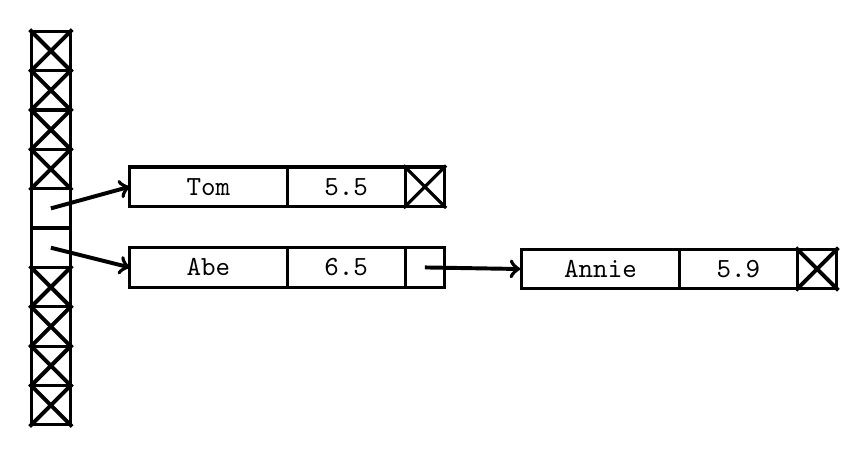
\begin{tikzpicture}
\draw[line width=0.05cm,black] (1.98,0.020000000000000018) to  (2.52,-0.52);
\draw[line width=0.05cm,black] (2.52,0.020000000000000018) to  (1.98,-0.52);
\draw[line width=0.05cm,black] (1.98,-0.48) to  (2.52,-1.02);
\draw[line width=0.05cm,black] (2.52,-0.48) to  (1.98,-1.02);
\draw[line width=0.05cm,black] (1.98,-0.98) to  (2.52,-1.52);
\draw[line width=0.05cm,black] (2.52,-0.98) to  (1.98,-1.52);
\draw[line width=0.05cm,black] (1.98,-1.48) to  (2.52,-2.02);
\draw[line width=0.05cm,black] (2.52,-1.48) to  (1.98,-2.02);

\draw (4.25, -1.975)
  node[draw, line width=0.04cm, , color=black,
       rounded corners=0cm, inner sep=0cm] {

\begin{minipage}[t][0.5cm]{2.0cm}
\mbox{}

\end{minipage}

};\draw (4.25, -1.975) node[color=black] {\texttt{Tom}};
\draw (6.0, -1.975)
  node[draw, line width=0.04cm, , color=black,
       rounded corners=0cm, inner sep=0cm] {

\begin{minipage}[t][0.5cm]{1.5cm}
\mbox{}

\end{minipage}

};\draw (6.0, -1.975) node[color=black] {\texttt{5.5}};
\draw (7.0, -1.975)
  node[draw, line width=0.04cm, , color=black,
       rounded corners=0cm, inner sep=0cm] {

\begin{minipage}[t][0.5cm]{0.5cm}
\mbox{}

\end{minipage}

};\draw[line width=0.05cm,black,->] (2.25,-2.25) to  (3.25,-1.9749999999999999);

\fill[black] (2.25, -2.25) circle (0);
\draw[black] (2.25, -2.25) circle (0.0);\draw[line width=0.04cm,black] (6.73,-1.705) to  (7.27,-2.245);
\draw[line width=0.04cm,black] (7.27,-1.705) to  (6.73,-2.245);

\draw (4.25, -3.0)
  node[draw, line width=0.04cm, , color=black,
       rounded corners=0cm, inner sep=0cm] {

\begin{minipage}[t][0.5cm]{2.0cm}
\mbox{}

\end{minipage}

};\draw (4.25, -3.0) node[color=black] {\texttt{Abe}};
\draw (6.0, -3.0)
  node[draw, line width=0.04cm, , color=black,
       rounded corners=0cm, inner sep=0cm] {

\begin{minipage}[t][0.5cm]{1.5cm}
\mbox{}

\end{minipage}

};\draw (6.0, -3.0) node[color=black] {\texttt{6.5}};
\draw (7.0, -3.0)
  node[draw, line width=0.04cm, , color=black,
       rounded corners=0cm, inner sep=0cm] {

\begin{minipage}[t][0.5cm]{0.5cm}
\mbox{}

\end{minipage}

};\draw[line width=0.05cm,black,->] (2.25,-2.75) to  (3.25,-3.0);

\fill[black] (2.25, -2.75) circle (0);
\draw[black] (2.25, -2.75) circle (0.0);
\draw (9.23, -3.02)
  node[draw, line width=0.04cm, , color=black,
       rounded corners=0cm, inner sep=0cm] {

\begin{minipage}[t][0.5cm]{2.0cm}
\mbox{}

\end{minipage}

};\draw (9.23, -3.02) node[color=black] {\texttt{Annie}};
\draw (10.98, -3.02)
  node[draw, line width=0.04cm, , color=black,
       rounded corners=0cm, inner sep=0cm] {

\begin{minipage}[t][0.5cm]{1.5cm}
\mbox{}

\end{minipage}

};\draw (10.98, -3.02) node[color=black] {\texttt{5.9}};
\draw (11.98, -3.02)
  node[draw, line width=0.04cm, , color=black,
       rounded corners=0cm, inner sep=0cm] {

\begin{minipage}[t][0.5cm]{0.5cm}
\mbox{}

\end{minipage}

};\draw[line width=0.05cm,black] (11.71,-2.75) to  (12.25,-3.29);
\draw[line width=0.05cm,black] (12.25,-2.75) to  (11.71,-3.29);
\draw[line width=0.05cm,black,->] (7.0,-3.0) to  (8.21,-3.0199999999999996);

\fill[black] (7.0, -3.0) circle (0);
\draw[black] (7.0, -3.0) circle (0.0);\draw[line width=0.05cm,black] (1.98,-2.98) to  (2.52,-3.52);
\draw[line width=0.05cm,black] (2.52,-2.98) to  (1.98,-3.52);
\draw[line width=0.05cm,black] (1.98,-3.4800000000000004) to  (2.52,-4.02);
\draw[line width=0.05cm,black] (2.52,-3.4800000000000004) to  (1.98,-4.02);
\draw[line width=0.05cm,black] (1.98,-3.9800000000000004) to  (2.52,-4.52);
\draw[line width=0.05cm,black] (2.52,-3.9800000000000004) to  (1.98,-4.52);
\draw[line width=0.05cm,black] (1.98,-4.48) to  (2.52,-5.02);
\draw[line width=0.05cm,black] (2.52,-4.48) to  (1.98,-5.02);

\draw (2.25, -0.25)
  node[draw, line width=0.04cm, , color=black,
       rounded corners=0cm, inner sep=0cm] {

\begin{minipage}[t][0.5cm]{0.5cm}
\mbox{}

\end{minipage}

};
\draw (2.25, -0.75)
  node[draw, line width=0.04cm, , color=black,
       rounded corners=0cm, inner sep=0cm] {

\begin{minipage}[t][0.5cm]{0.5cm}
\mbox{}

\end{minipage}

};
\draw (2.25, -1.25)
  node[draw, line width=0.04cm, , color=black,
       rounded corners=0cm, inner sep=0cm] {

\begin{minipage}[t][0.5cm]{0.5cm}
\mbox{}

\end{minipage}

};
\draw (2.25, -1.75)
  node[draw, line width=0.04cm, , color=black,
       rounded corners=0cm, inner sep=0cm] {

\begin{minipage}[t][0.5cm]{0.5cm}
\mbox{}

\end{minipage}

};
\draw (2.25, -2.25)
  node[draw, line width=0.04cm, , color=black,
       rounded corners=0cm, inner sep=0cm] {

\begin{minipage}[t][0.5cm]{0.5cm}
\mbox{}

\end{minipage}

};
\draw (2.25, -2.75)
  node[draw, line width=0.04cm, , color=black,
       rounded corners=0cm, inner sep=0cm] {

\begin{minipage}[t][0.5cm]{0.5cm}
\mbox{}

\end{minipage}

};
\draw (2.25, -3.25)
  node[draw, line width=0.04cm, , color=black,
       rounded corners=0cm, inner sep=0cm] {

\begin{minipage}[t][0.5cm]{0.5cm}
\mbox{}

\end{minipage}

};
\draw (2.25, -3.75)
  node[draw, line width=0.04cm, , color=black,
       rounded corners=0cm, inner sep=0cm] {

\begin{minipage}[t][0.5cm]{0.5cm}
\mbox{}

\end{minipage}

};
\draw (2.25, -4.25)
  node[draw, line width=0.04cm, , color=black,
       rounded corners=0cm, inner sep=0cm] {

\begin{minipage}[t][0.5cm]{0.5cm}
\mbox{}

\end{minipage}

};
\draw (2.25, -4.75)
  node[draw, line width=0.04cm, , color=black,
       rounded corners=0cm, inner sep=0cm] {

\begin{minipage}[t][0.5cm]{0.5cm}
\mbox{}

\end{minipage}

};
\end{tikzpicture}

\end{center}



Notice the patterns of the pairs of cells that contribute to the 
computation at $(3,2)$:
\begin{center}
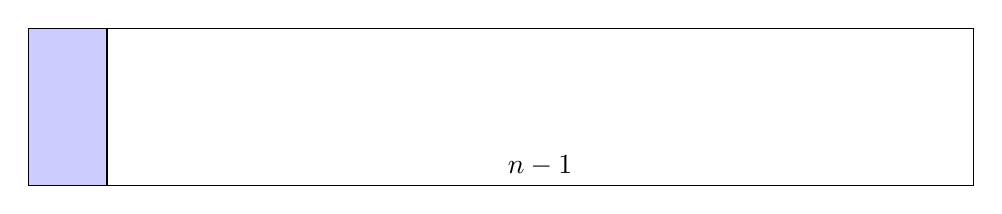
\begin{tikzpicture}

\draw (6.0, 1.0)
  node[draw, , , color=black,
       rounded corners=0cm, inner sep=0cm] {

\begin{minipage}[t][2cm]{12cm}
\mbox{}

\end{minipage}

};
\draw (0.5, 1.0)
  node[fill=blue!20!white,rounded corners=0cm,inner sep=0cm] {

\begin{minipage}[t][2cm]{1cm}
\mbox{}

\end{minipage}

};
\draw (0.5, 1.0)
  node[draw, , , color=black,
       rounded corners=0cm, inner sep=0cm] {

\begin{minipage}[t][2cm]{1cm}
\mbox{}

\end{minipage}

};
\draw (6.5, 0.25)
  node[draw=none, line width=0cm, , color=black,
       rounded corners=0cm, inner sep=0cm] {

\begin{minipage}[t][0.1cm]{0.1cm}
\mbox{}

\end{minipage}

};\draw (6.5, 0.25) node[color=black] {$n - 1$};
\end{tikzpicture}

\end{center}



Now following the same method, complete the second row yourself.

\[
  \text{[PAUSE]}
\]

\newpage
The table should now look like this:
\begin{center}
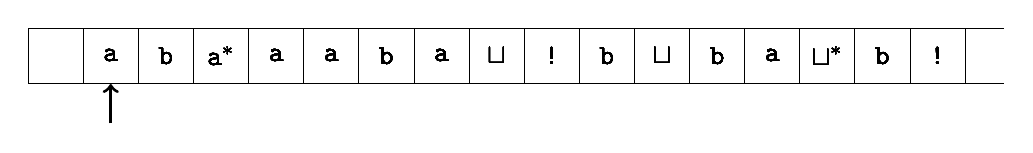
\begin{tikzpicture}

\draw (0.35, 0.35)
  node[draw, line width=0.01cm, , color=black,
       rounded corners=0cm, inner sep=0cm] {

\begin{minipage}[t][0.7cm]{0.7cm}
\mbox{}

\end{minipage}

};\draw (0.35, 0.35) node[color=black] {\texttt{\DOLLAR}};
\draw (1.0499999999999998, 0.35)
  node[draw, line width=0.01cm, , color=black,
       rounded corners=0cm, inner sep=0cm] {

\begin{minipage}[t][0.7cm]{0.7cm}
\mbox{}

\end{minipage}

};\draw (1.0499999999999998, 0.35) node[color=black] {\texttt{a}};
\draw (1.7499999999999998, 0.35)
  node[draw, line width=0.01cm, , color=black,
       rounded corners=0cm, inner sep=0cm] {

\begin{minipage}[t][0.7cm]{0.7cm}
\mbox{}

\end{minipage}

};\draw (1.7499999999999998, 0.35) node[color=black] {\texttt{b}};
\draw (2.4499999999999997, 0.35)
  node[draw, line width=0.01cm, , color=black,
       rounded corners=0cm, inner sep=0cm] {

\begin{minipage}[t][0.7cm]{0.7cm}
\mbox{}

\end{minipage}

};\draw (2.4499999999999997, 0.35) node[color=black] {\texttt{a$^*$}};
\draw (3.15, 0.35)
  node[draw, line width=0.01cm, , color=black,
       rounded corners=0cm, inner sep=0cm] {

\begin{minipage}[t][0.7cm]{0.7cm}
\mbox{}

\end{minipage}

};\draw (3.15, 0.35) node[color=black] {\texttt{a}};
\draw (3.85, 0.35)
  node[draw, line width=0.01cm, , color=black,
       rounded corners=0cm, inner sep=0cm] {

\begin{minipage}[t][0.7cm]{0.7cm}
\mbox{}

\end{minipage}

};\draw (3.85, 0.35) node[color=black] {\texttt{a}};
\draw (4.550000000000001, 0.35)
  node[draw, line width=0.01cm, , color=black,
       rounded corners=0cm, inner sep=0cm] {

\begin{minipage}[t][0.7cm]{0.7cm}
\mbox{}

\end{minipage}

};\draw (4.550000000000001, 0.35) node[color=black] {\texttt{b}};
\draw (5.25, 0.35)
  node[draw, line width=0.01cm, , color=black,
       rounded corners=0cm, inner sep=0cm] {

\begin{minipage}[t][0.7cm]{0.7cm}
\mbox{}

\end{minipage}

};\draw (5.25, 0.35) node[color=black] {\texttt{a}};
\draw (5.950000000000001, 0.35)
  node[draw, line width=0.01cm, , color=black,
       rounded corners=0cm, inner sep=0cm] {

\begin{minipage}[t][0.7cm]{0.7cm}
\mbox{}

\end{minipage}

};\draw (5.950000000000001, 0.35) node[color=black] {\texttt{$\sqcup$}};
\draw (6.65, 0.35)
  node[draw, line width=0.01cm, , color=black,
       rounded corners=0cm, inner sep=0cm] {

\begin{minipage}[t][0.7cm]{0.7cm}
\mbox{}

\end{minipage}

};\draw (6.65, 0.35) node[color=black] {\texttt{!}};
\draw (7.350000000000001, 0.35)
  node[draw, line width=0.01cm, , color=black,
       rounded corners=0cm, inner sep=0cm] {

\begin{minipage}[t][0.7cm]{0.7cm}
\mbox{}

\end{minipage}

};\draw (7.350000000000001, 0.35) node[color=black] {\texttt{b}};
\draw (8.05, 0.35)
  node[draw, line width=0.01cm, , color=black,
       rounded corners=0cm, inner sep=0cm] {

\begin{minipage}[t][0.7cm]{0.7cm}
\mbox{}

\end{minipage}

};\draw (8.05, 0.35) node[color=black] {\texttt{$\sqcup$}};
\draw (8.75, 0.35)
  node[draw, line width=0.01cm, , color=black,
       rounded corners=0cm, inner sep=0cm] {

\begin{minipage}[t][0.7cm]{0.7cm}
\mbox{}

\end{minipage}

};\draw (8.75, 0.35) node[color=black] {\texttt{b}};
\draw (9.45, 0.35)
  node[draw, line width=0.01cm, , color=black,
       rounded corners=0cm, inner sep=0cm] {

\begin{minipage}[t][0.7cm]{0.7cm}
\mbox{}

\end{minipage}

};\draw (9.45, 0.35) node[color=black] {\texttt{a}};
\draw (10.149999999999999, 0.35)
  node[draw, line width=0.01cm, , color=black,
       rounded corners=0cm, inner sep=0cm] {

\begin{minipage}[t][0.7cm]{0.7cm}
\mbox{}

\end{minipage}

};\draw (10.149999999999999, 0.35) node[color=black] {\texttt{$\sqcup^*$}};
\draw (10.849999999999998, 0.35)
  node[draw, line width=0.01cm, , color=black,
       rounded corners=0cm, inner sep=0cm] {

\begin{minipage}[t][0.7cm]{0.7cm}
\mbox{}

\end{minipage}

};\draw (10.849999999999998, 0.35) node[color=black] {\texttt{b}};
\draw (11.549999999999997, 0.35)
  node[draw, line width=0.01cm, , color=black,
       rounded corners=0cm, inner sep=0cm] {

\begin{minipage}[t][0.7cm]{0.7cm}
\mbox{}

\end{minipage}

};\draw (11.549999999999997, 0.35) node[color=black] {\texttt{!}};
\draw (0.35, 0.35)
  node[draw, line width=0.01cm, , color=black,
       rounded corners=0cm, inner sep=0cm] {

\begin{minipage}[t][0.7cm]{0.7cm}
\mbox{}

\end{minipage}

};\draw (0.35, 0.35) node[color=black] {\texttt{\DOLLAR}};
\draw (1.0499999999999998, 0.35)
  node[draw, line width=0.01cm, , color=black,
       rounded corners=0cm, inner sep=0cm] {

\begin{minipage}[t][0.7cm]{0.7cm}
\mbox{}

\end{minipage}

};\draw (1.0499999999999998, 0.35) node[color=black] {\texttt{a}};
\draw (1.7499999999999998, 0.35)
  node[draw, line width=0.01cm, , color=black,
       rounded corners=0cm, inner sep=0cm] {

\begin{minipage}[t][0.7cm]{0.7cm}
\mbox{}

\end{minipage}

};\draw (1.7499999999999998, 0.35) node[color=black] {\texttt{b}};
\draw (2.4499999999999997, 0.35)
  node[draw, line width=0.01cm, , color=black,
       rounded corners=0cm, inner sep=0cm] {

\begin{minipage}[t][0.7cm]{0.7cm}
\mbox{}

\end{minipage}

};\draw (2.4499999999999997, 0.35) node[color=black] {\texttt{a$^*$}};
\draw (3.15, 0.35)
  node[draw, line width=0.01cm, , color=black,
       rounded corners=0cm, inner sep=0cm] {

\begin{minipage}[t][0.7cm]{0.7cm}
\mbox{}

\end{minipage}

};\draw (3.15, 0.35) node[color=black] {\texttt{a}};
\draw (3.85, 0.35)
  node[draw, line width=0.01cm, , color=black,
       rounded corners=0cm, inner sep=0cm] {

\begin{minipage}[t][0.7cm]{0.7cm}
\mbox{}

\end{minipage}

};\draw (3.85, 0.35) node[color=black] {\texttt{a}};
\draw (4.550000000000001, 0.35)
  node[draw, line width=0.01cm, , color=black,
       rounded corners=0cm, inner sep=0cm] {

\begin{minipage}[t][0.7cm]{0.7cm}
\mbox{}

\end{minipage}

};\draw (4.550000000000001, 0.35) node[color=black] {\texttt{b}};
\draw (5.25, 0.35)
  node[draw, line width=0.01cm, , color=black,
       rounded corners=0cm, inner sep=0cm] {

\begin{minipage}[t][0.7cm]{0.7cm}
\mbox{}

\end{minipage}

};\draw (5.25, 0.35) node[color=black] {\texttt{a}};
\draw (5.950000000000001, 0.35)
  node[draw, line width=0.01cm, , color=black,
       rounded corners=0cm, inner sep=0cm] {

\begin{minipage}[t][0.7cm]{0.7cm}
\mbox{}

\end{minipage}

};\draw (5.950000000000001, 0.35) node[color=black] {\texttt{$\sqcup$}};
\draw (6.65, 0.35)
  node[draw, line width=0.01cm, , color=black,
       rounded corners=0cm, inner sep=0cm] {

\begin{minipage}[t][0.7cm]{0.7cm}
\mbox{}

\end{minipage}

};\draw (6.65, 0.35) node[color=black] {\texttt{!}};
\draw (7.350000000000001, 0.35)
  node[draw, line width=0.01cm, , color=black,
       rounded corners=0cm, inner sep=0cm] {

\begin{minipage}[t][0.7cm]{0.7cm}
\mbox{}

\end{minipage}

};\draw (7.350000000000001, 0.35) node[color=black] {\texttt{b}};
\draw (8.05, 0.35)
  node[draw, line width=0.01cm, , color=black,
       rounded corners=0cm, inner sep=0cm] {

\begin{minipage}[t][0.7cm]{0.7cm}
\mbox{}

\end{minipage}

};\draw (8.05, 0.35) node[color=black] {\texttt{$\sqcup$}};
\draw (8.75, 0.35)
  node[draw, line width=0.01cm, , color=black,
       rounded corners=0cm, inner sep=0cm] {

\begin{minipage}[t][0.7cm]{0.7cm}
\mbox{}

\end{minipage}

};\draw (8.75, 0.35) node[color=black] {\texttt{b}};
\draw (9.45, 0.35)
  node[draw, line width=0.01cm, , color=black,
       rounded corners=0cm, inner sep=0cm] {

\begin{minipage}[t][0.7cm]{0.7cm}
\mbox{}

\end{minipage}

};\draw (9.45, 0.35) node[color=black] {\texttt{a}};
\draw (10.149999999999999, 0.35)
  node[draw, line width=0.01cm, , color=black,
       rounded corners=0cm, inner sep=0cm] {

\begin{minipage}[t][0.7cm]{0.7cm}
\mbox{}

\end{minipage}

};\draw (10.149999999999999, 0.35) node[color=black] {\texttt{$\sqcup^*$}};
\draw (10.849999999999998, 0.35)
  node[draw, line width=0.01cm, , color=black,
       rounded corners=0cm, inner sep=0cm] {

\begin{minipage}[t][0.7cm]{0.7cm}
\mbox{}

\end{minipage}

};\draw (10.849999999999998, 0.35) node[color=black] {\texttt{b}};
\draw (11.549999999999997, 0.35)
  node[draw, line width=0.01cm, , color=black,
       rounded corners=0cm, inner sep=0cm] {

\begin{minipage}[t][0.7cm]{0.7cm}
\mbox{}

\end{minipage}

};\draw (11.549999999999997, 0.35) node[color=black] {\texttt{!}};
\draw (0.35, 0.35)
  node[draw, line width=0.01cm, , color=black,
       rounded corners=0cm, inner sep=0cm] {

\begin{minipage}[t][0.7cm]{0.7cm}
\mbox{}

\end{minipage}

};\draw (0.35, 0.35) node[color=black] {\texttt{\DOLLAR}};
\draw (1.0499999999999998, 0.35)
  node[draw, line width=0.01cm, , color=black,
       rounded corners=0cm, inner sep=0cm] {

\begin{minipage}[t][0.7cm]{0.7cm}
\mbox{}

\end{minipage}

};\draw (1.0499999999999998, 0.35) node[color=black] {\texttt{a}};
\draw (1.7499999999999998, 0.35)
  node[draw, line width=0.01cm, , color=black,
       rounded corners=0cm, inner sep=0cm] {

\begin{minipage}[t][0.7cm]{0.7cm}
\mbox{}

\end{minipage}

};\draw (1.7499999999999998, 0.35) node[color=black] {\texttt{b}};
\draw (2.4499999999999997, 0.35)
  node[draw, line width=0.01cm, , color=black,
       rounded corners=0cm, inner sep=0cm] {

\begin{minipage}[t][0.7cm]{0.7cm}
\mbox{}

\end{minipage}

};\draw (2.4499999999999997, 0.35) node[color=black] {\texttt{a$^*$}};
\draw (3.15, 0.35)
  node[draw, line width=0.01cm, , color=black,
       rounded corners=0cm, inner sep=0cm] {

\begin{minipage}[t][0.7cm]{0.7cm}
\mbox{}

\end{minipage}

};\draw (3.15, 0.35) node[color=black] {\texttt{a}};
\draw (3.85, 0.35)
  node[draw, line width=0.01cm, , color=black,
       rounded corners=0cm, inner sep=0cm] {

\begin{minipage}[t][0.7cm]{0.7cm}
\mbox{}

\end{minipage}

};\draw (3.85, 0.35) node[color=black] {\texttt{a}};
\draw (4.550000000000001, 0.35)
  node[draw, line width=0.01cm, , color=black,
       rounded corners=0cm, inner sep=0cm] {

\begin{minipage}[t][0.7cm]{0.7cm}
\mbox{}

\end{minipage}

};\draw (4.550000000000001, 0.35) node[color=black] {\texttt{b}};
\draw (5.25, 0.35)
  node[draw, line width=0.01cm, , color=black,
       rounded corners=0cm, inner sep=0cm] {

\begin{minipage}[t][0.7cm]{0.7cm}
\mbox{}

\end{minipage}

};\draw (5.25, 0.35) node[color=black] {\texttt{a}};
\draw (5.950000000000001, 0.35)
  node[draw, line width=0.01cm, , color=black,
       rounded corners=0cm, inner sep=0cm] {

\begin{minipage}[t][0.7cm]{0.7cm}
\mbox{}

\end{minipage}

};\draw (5.950000000000001, 0.35) node[color=black] {\texttt{$\sqcup$}};
\draw (6.65, 0.35)
  node[draw, line width=0.01cm, , color=black,
       rounded corners=0cm, inner sep=0cm] {

\begin{minipage}[t][0.7cm]{0.7cm}
\mbox{}

\end{minipage}

};\draw (6.65, 0.35) node[color=black] {\texttt{!}};
\draw (7.350000000000001, 0.35)
  node[draw, line width=0.01cm, , color=black,
       rounded corners=0cm, inner sep=0cm] {

\begin{minipage}[t][0.7cm]{0.7cm}
\mbox{}

\end{minipage}

};\draw (7.350000000000001, 0.35) node[color=black] {\texttt{b}};
\draw (8.05, 0.35)
  node[draw, line width=0.01cm, , color=black,
       rounded corners=0cm, inner sep=0cm] {

\begin{minipage}[t][0.7cm]{0.7cm}
\mbox{}

\end{minipage}

};\draw (8.05, 0.35) node[color=black] {\texttt{$\sqcup$}};
\draw (8.75, 0.35)
  node[draw, line width=0.01cm, , color=black,
       rounded corners=0cm, inner sep=0cm] {

\begin{minipage}[t][0.7cm]{0.7cm}
\mbox{}

\end{minipage}

};\draw (8.75, 0.35) node[color=black] {\texttt{b}};
\draw (9.45, 0.35)
  node[draw, line width=0.01cm, , color=black,
       rounded corners=0cm, inner sep=0cm] {

\begin{minipage}[t][0.7cm]{0.7cm}
\mbox{}

\end{minipage}

};\draw (9.45, 0.35) node[color=black] {\texttt{a}};
\draw (10.149999999999999, 0.35)
  node[draw, line width=0.01cm, , color=black,
       rounded corners=0cm, inner sep=0cm] {

\begin{minipage}[t][0.7cm]{0.7cm}
\mbox{}

\end{minipage}

};\draw (10.149999999999999, 0.35) node[color=black] {\texttt{$\sqcup^*$}};
\draw (10.849999999999998, 0.35)
  node[draw, line width=0.01cm, , color=black,
       rounded corners=0cm, inner sep=0cm] {

\begin{minipage}[t][0.7cm]{0.7cm}
\mbox{}

\end{minipage}

};\draw (10.849999999999998, 0.35) node[color=black] {\texttt{b}};
\draw (11.549999999999997, 0.35)
  node[draw, line width=0.01cm, , color=black,
       rounded corners=0cm, inner sep=0cm] {

\begin{minipage}[t][0.7cm]{0.7cm}
\mbox{}

\end{minipage}

};\draw (11.549999999999997, 0.35) node[color=black] {\texttt{!}};
\draw (0.35, 0.35)
  node[draw, line width=0.01cm, , color=black,
       rounded corners=0cm, inner sep=0cm] {

\begin{minipage}[t][0.7cm]{0.7cm}
\mbox{}

\end{minipage}

};\draw (0.35, 0.35) node[color=black] {\texttt{\DOLLAR}};
\draw (1.0499999999999998, 0.35)
  node[draw, line width=0.01cm, , color=black,
       rounded corners=0cm, inner sep=0cm] {

\begin{minipage}[t][0.7cm]{0.7cm}
\mbox{}

\end{minipage}

};\draw (1.0499999999999998, 0.35) node[color=black] {\texttt{a}};
\draw (1.7499999999999998, 0.35)
  node[draw, line width=0.01cm, , color=black,
       rounded corners=0cm, inner sep=0cm] {

\begin{minipage}[t][0.7cm]{0.7cm}
\mbox{}

\end{minipage}

};\draw (1.7499999999999998, 0.35) node[color=black] {\texttt{b}};
\draw (2.4499999999999997, 0.35)
  node[draw, line width=0.01cm, , color=black,
       rounded corners=0cm, inner sep=0cm] {

\begin{minipage}[t][0.7cm]{0.7cm}
\mbox{}

\end{minipage}

};\draw (2.4499999999999997, 0.35) node[color=black] {\texttt{a$^*$}};
\draw (3.15, 0.35)
  node[draw, line width=0.01cm, , color=black,
       rounded corners=0cm, inner sep=0cm] {

\begin{minipage}[t][0.7cm]{0.7cm}
\mbox{}

\end{minipage}

};\draw (3.15, 0.35) node[color=black] {\texttt{a}};
\draw (3.85, 0.35)
  node[draw, line width=0.01cm, , color=black,
       rounded corners=0cm, inner sep=0cm] {

\begin{minipage}[t][0.7cm]{0.7cm}
\mbox{}

\end{minipage}

};\draw (3.85, 0.35) node[color=black] {\texttt{a}};
\draw (4.550000000000001, 0.35)
  node[draw, line width=0.01cm, , color=black,
       rounded corners=0cm, inner sep=0cm] {

\begin{minipage}[t][0.7cm]{0.7cm}
\mbox{}

\end{minipage}

};\draw (4.550000000000001, 0.35) node[color=black] {\texttt{b}};
\draw (5.25, 0.35)
  node[draw, line width=0.01cm, , color=black,
       rounded corners=0cm, inner sep=0cm] {

\begin{minipage}[t][0.7cm]{0.7cm}
\mbox{}

\end{minipage}

};\draw (5.25, 0.35) node[color=black] {\texttt{a}};
\draw (5.950000000000001, 0.35)
  node[draw, line width=0.01cm, , color=black,
       rounded corners=0cm, inner sep=0cm] {

\begin{minipage}[t][0.7cm]{0.7cm}
\mbox{}

\end{minipage}

};\draw (5.950000000000001, 0.35) node[color=black] {\texttt{$\sqcup$}};
\draw (6.65, 0.35)
  node[draw, line width=0.01cm, , color=black,
       rounded corners=0cm, inner sep=0cm] {

\begin{minipage}[t][0.7cm]{0.7cm}
\mbox{}

\end{minipage}

};\draw (6.65, 0.35) node[color=black] {\texttt{!}};
\draw (7.350000000000001, 0.35)
  node[draw, line width=0.01cm, , color=black,
       rounded corners=0cm, inner sep=0cm] {

\begin{minipage}[t][0.7cm]{0.7cm}
\mbox{}

\end{minipage}

};\draw (7.350000000000001, 0.35) node[color=black] {\texttt{b}};
\draw (8.05, 0.35)
  node[draw, line width=0.01cm, , color=black,
       rounded corners=0cm, inner sep=0cm] {

\begin{minipage}[t][0.7cm]{0.7cm}
\mbox{}

\end{minipage}

};\draw (8.05, 0.35) node[color=black] {\texttt{$\sqcup$}};
\draw (8.75, 0.35)
  node[draw, line width=0.01cm, , color=black,
       rounded corners=0cm, inner sep=0cm] {

\begin{minipage}[t][0.7cm]{0.7cm}
\mbox{}

\end{minipage}

};\draw (8.75, 0.35) node[color=black] {\texttt{b}};
\draw (9.45, 0.35)
  node[draw, line width=0.01cm, , color=black,
       rounded corners=0cm, inner sep=0cm] {

\begin{minipage}[t][0.7cm]{0.7cm}
\mbox{}

\end{minipage}

};\draw (9.45, 0.35) node[color=black] {\texttt{a}};
\draw (10.149999999999999, 0.35)
  node[draw, line width=0.01cm, , color=black,
       rounded corners=0cm, inner sep=0cm] {

\begin{minipage}[t][0.7cm]{0.7cm}
\mbox{}

\end{minipage}

};\draw (10.149999999999999, 0.35) node[color=black] {\texttt{$\sqcup^*$}};
\draw (10.849999999999998, 0.35)
  node[draw, line width=0.01cm, , color=black,
       rounded corners=0cm, inner sep=0cm] {

\begin{minipage}[t][0.7cm]{0.7cm}
\mbox{}

\end{minipage}

};\draw (10.849999999999998, 0.35) node[color=black] {\texttt{b}};
\draw (11.549999999999997, 0.35)
  node[draw, line width=0.01cm, , color=black,
       rounded corners=0cm, inner sep=0cm] {

\begin{minipage}[t][0.7cm]{0.7cm}
\mbox{}

\end{minipage}

};\draw (11.549999999999997, 0.35) node[color=black] {\texttt{!}};
\draw (0.35, 0.35)
  node[draw, line width=0.01cm, , color=black,
       rounded corners=0cm, inner sep=0cm] {

\begin{minipage}[t][0.7cm]{0.7cm}
\mbox{}

\end{minipage}

};\draw (0.35, 0.35) node[color=black] {\texttt{\DOLLAR}};
\draw (1.0499999999999998, 0.35)
  node[draw, line width=0.01cm, , color=black,
       rounded corners=0cm, inner sep=0cm] {

\begin{minipage}[t][0.7cm]{0.7cm}
\mbox{}

\end{minipage}

};\draw (1.0499999999999998, 0.35) node[color=black] {\texttt{a}};
\draw (1.7499999999999998, 0.35)
  node[draw, line width=0.01cm, , color=black,
       rounded corners=0cm, inner sep=0cm] {

\begin{minipage}[t][0.7cm]{0.7cm}
\mbox{}

\end{minipage}

};\draw (1.7499999999999998, 0.35) node[color=black] {\texttt{b}};
\draw (2.4499999999999997, 0.35)
  node[draw, line width=0.01cm, , color=black,
       rounded corners=0cm, inner sep=0cm] {

\begin{minipage}[t][0.7cm]{0.7cm}
\mbox{}

\end{minipage}

};\draw (2.4499999999999997, 0.35) node[color=black] {\texttt{a$^*$}};
\draw (3.15, 0.35)
  node[draw, line width=0.01cm, , color=black,
       rounded corners=0cm, inner sep=0cm] {

\begin{minipage}[t][0.7cm]{0.7cm}
\mbox{}

\end{minipage}

};\draw (3.15, 0.35) node[color=black] {\texttt{a}};
\draw (3.85, 0.35)
  node[draw, line width=0.01cm, , color=black,
       rounded corners=0cm, inner sep=0cm] {

\begin{minipage}[t][0.7cm]{0.7cm}
\mbox{}

\end{minipage}

};\draw (3.85, 0.35) node[color=black] {\texttt{a}};
\draw (4.550000000000001, 0.35)
  node[draw, line width=0.01cm, , color=black,
       rounded corners=0cm, inner sep=0cm] {

\begin{minipage}[t][0.7cm]{0.7cm}
\mbox{}

\end{minipage}

};\draw (4.550000000000001, 0.35) node[color=black] {\texttt{b}};
\draw (5.25, 0.35)
  node[draw, line width=0.01cm, , color=black,
       rounded corners=0cm, inner sep=0cm] {

\begin{minipage}[t][0.7cm]{0.7cm}
\mbox{}

\end{minipage}

};\draw (5.25, 0.35) node[color=black] {\texttt{a}};
\draw (5.950000000000001, 0.35)
  node[draw, line width=0.01cm, , color=black,
       rounded corners=0cm, inner sep=0cm] {

\begin{minipage}[t][0.7cm]{0.7cm}
\mbox{}

\end{minipage}

};\draw (5.950000000000001, 0.35) node[color=black] {\texttt{$\sqcup$}};
\draw (6.65, 0.35)
  node[draw, line width=0.01cm, , color=black,
       rounded corners=0cm, inner sep=0cm] {

\begin{minipage}[t][0.7cm]{0.7cm}
\mbox{}

\end{minipage}

};\draw (6.65, 0.35) node[color=black] {\texttt{!}};
\draw (7.350000000000001, 0.35)
  node[draw, line width=0.01cm, , color=black,
       rounded corners=0cm, inner sep=0cm] {

\begin{minipage}[t][0.7cm]{0.7cm}
\mbox{}

\end{minipage}

};\draw (7.350000000000001, 0.35) node[color=black] {\texttt{b}};
\draw (8.05, 0.35)
  node[draw, line width=0.01cm, , color=black,
       rounded corners=0cm, inner sep=0cm] {

\begin{minipage}[t][0.7cm]{0.7cm}
\mbox{}

\end{minipage}

};\draw (8.05, 0.35) node[color=black] {\texttt{$\sqcup$}};
\draw (8.75, 0.35)
  node[draw, line width=0.01cm, , color=black,
       rounded corners=0cm, inner sep=0cm] {

\begin{minipage}[t][0.7cm]{0.7cm}
\mbox{}

\end{minipage}

};\draw (8.75, 0.35) node[color=black] {\texttt{b}};
\draw (9.45, 0.35)
  node[draw, line width=0.01cm, , color=black,
       rounded corners=0cm, inner sep=0cm] {

\begin{minipage}[t][0.7cm]{0.7cm}
\mbox{}

\end{minipage}

};\draw (9.45, 0.35) node[color=black] {\texttt{a}};
\draw (10.149999999999999, 0.35)
  node[draw, line width=0.01cm, , color=black,
       rounded corners=0cm, inner sep=0cm] {

\begin{minipage}[t][0.7cm]{0.7cm}
\mbox{}

\end{minipage}

};\draw (10.149999999999999, 0.35) node[color=black] {\texttt{$\sqcup^*$}};
\draw (10.849999999999998, 0.35)
  node[draw, line width=0.01cm, , color=black,
       rounded corners=0cm, inner sep=0cm] {

\begin{minipage}[t][0.7cm]{0.7cm}
\mbox{}

\end{minipage}

};\draw (10.849999999999998, 0.35) node[color=black] {\texttt{b}};
\draw (11.549999999999997, 0.35)
  node[draw, line width=0.01cm, , color=black,
       rounded corners=0cm, inner sep=0cm] {

\begin{minipage}[t][0.7cm]{0.7cm}
\mbox{}

\end{minipage}

};\draw (11.549999999999997, 0.35) node[color=black] {\texttt{!}};
\draw (0.35, 0.35)
  node[draw, line width=0.01cm, , color=black,
       rounded corners=0cm, inner sep=0cm] {

\begin{minipage}[t][0.7cm]{0.7cm}
\mbox{}

\end{minipage}

};\draw (0.35, 0.35) node[color=black] {\texttt{\DOLLAR}};
\draw (1.0499999999999998, 0.35)
  node[draw, line width=0.01cm, , color=black,
       rounded corners=0cm, inner sep=0cm] {

\begin{minipage}[t][0.7cm]{0.7cm}
\mbox{}

\end{minipage}

};\draw (1.0499999999999998, 0.35) node[color=black] {\texttt{a}};
\draw (1.7499999999999998, 0.35)
  node[draw, line width=0.01cm, , color=black,
       rounded corners=0cm, inner sep=0cm] {

\begin{minipage}[t][0.7cm]{0.7cm}
\mbox{}

\end{minipage}

};\draw (1.7499999999999998, 0.35) node[color=black] {\texttt{b}};
\draw (2.4499999999999997, 0.35)
  node[draw, line width=0.01cm, , color=black,
       rounded corners=0cm, inner sep=0cm] {

\begin{minipage}[t][0.7cm]{0.7cm}
\mbox{}

\end{minipage}

};\draw (2.4499999999999997, 0.35) node[color=black] {\texttt{a$^*$}};
\draw (3.15, 0.35)
  node[draw, line width=0.01cm, , color=black,
       rounded corners=0cm, inner sep=0cm] {

\begin{minipage}[t][0.7cm]{0.7cm}
\mbox{}

\end{minipage}

};\draw (3.15, 0.35) node[color=black] {\texttt{a}};
\draw (3.85, 0.35)
  node[draw, line width=0.01cm, , color=black,
       rounded corners=0cm, inner sep=0cm] {

\begin{minipage}[t][0.7cm]{0.7cm}
\mbox{}

\end{minipage}

};\draw (3.85, 0.35) node[color=black] {\texttt{a}};
\draw (4.550000000000001, 0.35)
  node[draw, line width=0.01cm, , color=black,
       rounded corners=0cm, inner sep=0cm] {

\begin{minipage}[t][0.7cm]{0.7cm}
\mbox{}

\end{minipage}

};\draw (4.550000000000001, 0.35) node[color=black] {\texttt{b}};
\draw (5.25, 0.35)
  node[draw, line width=0.01cm, , color=black,
       rounded corners=0cm, inner sep=0cm] {

\begin{minipage}[t][0.7cm]{0.7cm}
\mbox{}

\end{minipage}

};\draw (5.25, 0.35) node[color=black] {\texttt{a}};
\draw (5.950000000000001, 0.35)
  node[draw, line width=0.01cm, , color=black,
       rounded corners=0cm, inner sep=0cm] {

\begin{minipage}[t][0.7cm]{0.7cm}
\mbox{}

\end{minipage}

};\draw (5.950000000000001, 0.35) node[color=black] {\texttt{$\sqcup$}};
\draw (6.65, 0.35)
  node[draw, line width=0.01cm, , color=black,
       rounded corners=0cm, inner sep=0cm] {

\begin{minipage}[t][0.7cm]{0.7cm}
\mbox{}

\end{minipage}

};\draw (6.65, 0.35) node[color=black] {\texttt{!}};
\draw (7.350000000000001, 0.35)
  node[draw, line width=0.01cm, , color=black,
       rounded corners=0cm, inner sep=0cm] {

\begin{minipage}[t][0.7cm]{0.7cm}
\mbox{}

\end{minipage}

};\draw (7.350000000000001, 0.35) node[color=black] {\texttt{b}};
\draw (8.05, 0.35)
  node[draw, line width=0.01cm, , color=black,
       rounded corners=0cm, inner sep=0cm] {

\begin{minipage}[t][0.7cm]{0.7cm}
\mbox{}

\end{minipage}

};\draw (8.05, 0.35) node[color=black] {\texttt{$\sqcup$}};
\draw (8.75, 0.35)
  node[draw, line width=0.01cm, , color=black,
       rounded corners=0cm, inner sep=0cm] {

\begin{minipage}[t][0.7cm]{0.7cm}
\mbox{}

\end{minipage}

};\draw (8.75, 0.35) node[color=black] {\texttt{b}};
\draw (9.45, 0.35)
  node[draw, line width=0.01cm, , color=black,
       rounded corners=0cm, inner sep=0cm] {

\begin{minipage}[t][0.7cm]{0.7cm}
\mbox{}

\end{minipage}

};\draw (9.45, 0.35) node[color=black] {\texttt{a}};
\draw (10.149999999999999, 0.35)
  node[draw, line width=0.01cm, , color=black,
       rounded corners=0cm, inner sep=0cm] {

\begin{minipage}[t][0.7cm]{0.7cm}
\mbox{}

\end{minipage}

};\draw (10.149999999999999, 0.35) node[color=black] {\texttt{$\sqcup^*$}};
\draw (10.849999999999998, 0.35)
  node[draw, line width=0.01cm, , color=black,
       rounded corners=0cm, inner sep=0cm] {

\begin{minipage}[t][0.7cm]{0.7cm}
\mbox{}

\end{minipage}

};\draw (10.849999999999998, 0.35) node[color=black] {\texttt{b}};
\draw (11.549999999999997, 0.35)
  node[draw, line width=0.01cm, , color=black,
       rounded corners=0cm, inner sep=0cm] {

\begin{minipage}[t][0.7cm]{0.7cm}
\mbox{}

\end{minipage}

};\draw (11.549999999999997, 0.35) node[color=black] {\texttt{!}};
\draw (0.35, 0.35)
  node[draw, line width=0.01cm, , color=black,
       rounded corners=0cm, inner sep=0cm] {

\begin{minipage}[t][0.7cm]{0.7cm}
\mbox{}

\end{minipage}

};\draw (0.35, 0.35) node[color=black] {\texttt{\DOLLAR}};
\draw (1.0499999999999998, 0.35)
  node[draw, line width=0.01cm, , color=black,
       rounded corners=0cm, inner sep=0cm] {

\begin{minipage}[t][0.7cm]{0.7cm}
\mbox{}

\end{minipage}

};\draw (1.0499999999999998, 0.35) node[color=black] {\texttt{a}};
\draw (1.7499999999999998, 0.35)
  node[draw, line width=0.01cm, , color=black,
       rounded corners=0cm, inner sep=0cm] {

\begin{minipage}[t][0.7cm]{0.7cm}
\mbox{}

\end{minipage}

};\draw (1.7499999999999998, 0.35) node[color=black] {\texttt{b}};
\draw (2.4499999999999997, 0.35)
  node[draw, line width=0.01cm, , color=black,
       rounded corners=0cm, inner sep=0cm] {

\begin{minipage}[t][0.7cm]{0.7cm}
\mbox{}

\end{minipage}

};\draw (2.4499999999999997, 0.35) node[color=black] {\texttt{a$^*$}};
\draw (3.15, 0.35)
  node[draw, line width=0.01cm, , color=black,
       rounded corners=0cm, inner sep=0cm] {

\begin{minipage}[t][0.7cm]{0.7cm}
\mbox{}

\end{minipage}

};\draw (3.15, 0.35) node[color=black] {\texttt{a}};
\draw (3.85, 0.35)
  node[draw, line width=0.01cm, , color=black,
       rounded corners=0cm, inner sep=0cm] {

\begin{minipage}[t][0.7cm]{0.7cm}
\mbox{}

\end{minipage}

};\draw (3.85, 0.35) node[color=black] {\texttt{a}};
\draw (4.550000000000001, 0.35)
  node[draw, line width=0.01cm, , color=black,
       rounded corners=0cm, inner sep=0cm] {

\begin{minipage}[t][0.7cm]{0.7cm}
\mbox{}

\end{minipage}

};\draw (4.550000000000001, 0.35) node[color=black] {\texttt{b}};
\draw (5.25, 0.35)
  node[draw, line width=0.01cm, , color=black,
       rounded corners=0cm, inner sep=0cm] {

\begin{minipage}[t][0.7cm]{0.7cm}
\mbox{}

\end{minipage}

};\draw (5.25, 0.35) node[color=black] {\texttt{a}};
\draw (5.950000000000001, 0.35)
  node[draw, line width=0.01cm, , color=black,
       rounded corners=0cm, inner sep=0cm] {

\begin{minipage}[t][0.7cm]{0.7cm}
\mbox{}

\end{minipage}

};\draw (5.950000000000001, 0.35) node[color=black] {\texttt{$\sqcup$}};
\draw (6.65, 0.35)
  node[draw, line width=0.01cm, , color=black,
       rounded corners=0cm, inner sep=0cm] {

\begin{minipage}[t][0.7cm]{0.7cm}
\mbox{}

\end{minipage}

};\draw (6.65, 0.35) node[color=black] {\texttt{!}};
\draw (7.350000000000001, 0.35)
  node[draw, line width=0.01cm, , color=black,
       rounded corners=0cm, inner sep=0cm] {

\begin{minipage}[t][0.7cm]{0.7cm}
\mbox{}

\end{minipage}

};\draw (7.350000000000001, 0.35) node[color=black] {\texttt{b}};
\draw (8.05, 0.35)
  node[draw, line width=0.01cm, , color=black,
       rounded corners=0cm, inner sep=0cm] {

\begin{minipage}[t][0.7cm]{0.7cm}
\mbox{}

\end{minipage}

};\draw (8.05, 0.35) node[color=black] {\texttt{$\sqcup$}};
\draw (8.75, 0.35)
  node[draw, line width=0.01cm, , color=black,
       rounded corners=0cm, inner sep=0cm] {

\begin{minipage}[t][0.7cm]{0.7cm}
\mbox{}

\end{minipage}

};\draw (8.75, 0.35) node[color=black] {\texttt{b}};
\draw (9.45, 0.35)
  node[draw, line width=0.01cm, , color=black,
       rounded corners=0cm, inner sep=0cm] {

\begin{minipage}[t][0.7cm]{0.7cm}
\mbox{}

\end{minipage}

};\draw (9.45, 0.35) node[color=black] {\texttt{a}};
\draw (10.149999999999999, 0.35)
  node[draw, line width=0.01cm, , color=black,
       rounded corners=0cm, inner sep=0cm] {

\begin{minipage}[t][0.7cm]{0.7cm}
\mbox{}

\end{minipage}

};\draw (10.149999999999999, 0.35) node[color=black] {\texttt{$\sqcup^*$}};
\draw (10.849999999999998, 0.35)
  node[draw, line width=0.01cm, , color=black,
       rounded corners=0cm, inner sep=0cm] {

\begin{minipage}[t][0.7cm]{0.7cm}
\mbox{}

\end{minipage}

};\draw (10.849999999999998, 0.35) node[color=black] {\texttt{b}};
\draw (11.549999999999997, 0.35)
  node[draw, line width=0.01cm, , color=black,
       rounded corners=0cm, inner sep=0cm] {

\begin{minipage}[t][0.7cm]{0.7cm}
\mbox{}

\end{minipage}

};\draw (11.549999999999997, 0.35) node[color=black] {\texttt{!}};
\draw (0.35, 0.35)
  node[draw, line width=0.01cm, , color=black,
       rounded corners=0cm, inner sep=0cm] {

\begin{minipage}[t][0.7cm]{0.7cm}
\mbox{}

\end{minipage}

};\draw (0.35, 0.35) node[color=black] {\texttt{\DOLLAR}};
\draw (1.0499999999999998, 0.35)
  node[draw, line width=0.01cm, , color=black,
       rounded corners=0cm, inner sep=0cm] {

\begin{minipage}[t][0.7cm]{0.7cm}
\mbox{}

\end{minipage}

};\draw (1.0499999999999998, 0.35) node[color=black] {\texttt{a}};
\draw (1.7499999999999998, 0.35)
  node[draw, line width=0.01cm, , color=black,
       rounded corners=0cm, inner sep=0cm] {

\begin{minipage}[t][0.7cm]{0.7cm}
\mbox{}

\end{minipage}

};\draw (1.7499999999999998, 0.35) node[color=black] {\texttt{b}};
\draw (2.4499999999999997, 0.35)
  node[draw, line width=0.01cm, , color=black,
       rounded corners=0cm, inner sep=0cm] {

\begin{minipage}[t][0.7cm]{0.7cm}
\mbox{}

\end{minipage}

};\draw (2.4499999999999997, 0.35) node[color=black] {\texttt{a$^*$}};
\draw (3.15, 0.35)
  node[draw, line width=0.01cm, , color=black,
       rounded corners=0cm, inner sep=0cm] {

\begin{minipage}[t][0.7cm]{0.7cm}
\mbox{}

\end{minipage}

};\draw (3.15, 0.35) node[color=black] {\texttt{a}};
\draw (3.85, 0.35)
  node[draw, line width=0.01cm, , color=black,
       rounded corners=0cm, inner sep=0cm] {

\begin{minipage}[t][0.7cm]{0.7cm}
\mbox{}

\end{minipage}

};\draw (3.85, 0.35) node[color=black] {\texttt{a}};
\draw (4.550000000000001, 0.35)
  node[draw, line width=0.01cm, , color=black,
       rounded corners=0cm, inner sep=0cm] {

\begin{minipage}[t][0.7cm]{0.7cm}
\mbox{}

\end{minipage}

};\draw (4.550000000000001, 0.35) node[color=black] {\texttt{b}};
\draw (5.25, 0.35)
  node[draw, line width=0.01cm, , color=black,
       rounded corners=0cm, inner sep=0cm] {

\begin{minipage}[t][0.7cm]{0.7cm}
\mbox{}

\end{minipage}

};\draw (5.25, 0.35) node[color=black] {\texttt{a}};
\draw (5.950000000000001, 0.35)
  node[draw, line width=0.01cm, , color=black,
       rounded corners=0cm, inner sep=0cm] {

\begin{minipage}[t][0.7cm]{0.7cm}
\mbox{}

\end{minipage}

};\draw (5.950000000000001, 0.35) node[color=black] {\texttt{$\sqcup$}};
\draw (6.65, 0.35)
  node[draw, line width=0.01cm, , color=black,
       rounded corners=0cm, inner sep=0cm] {

\begin{minipage}[t][0.7cm]{0.7cm}
\mbox{}

\end{minipage}

};\draw (6.65, 0.35) node[color=black] {\texttt{!}};
\draw (7.350000000000001, 0.35)
  node[draw, line width=0.01cm, , color=black,
       rounded corners=0cm, inner sep=0cm] {

\begin{minipage}[t][0.7cm]{0.7cm}
\mbox{}

\end{minipage}

};\draw (7.350000000000001, 0.35) node[color=black] {\texttt{b}};
\draw (8.05, 0.35)
  node[draw, line width=0.01cm, , color=black,
       rounded corners=0cm, inner sep=0cm] {

\begin{minipage}[t][0.7cm]{0.7cm}
\mbox{}

\end{minipage}

};\draw (8.05, 0.35) node[color=black] {\texttt{$\sqcup$}};
\draw (8.75, 0.35)
  node[draw, line width=0.01cm, , color=black,
       rounded corners=0cm, inner sep=0cm] {

\begin{minipage}[t][0.7cm]{0.7cm}
\mbox{}

\end{minipage}

};\draw (8.75, 0.35) node[color=black] {\texttt{b}};
\draw (9.45, 0.35)
  node[draw, line width=0.01cm, , color=black,
       rounded corners=0cm, inner sep=0cm] {

\begin{minipage}[t][0.7cm]{0.7cm}
\mbox{}

\end{minipage}

};\draw (9.45, 0.35) node[color=black] {\texttt{a}};
\draw (10.149999999999999, 0.35)
  node[draw, line width=0.01cm, , color=black,
       rounded corners=0cm, inner sep=0cm] {

\begin{minipage}[t][0.7cm]{0.7cm}
\mbox{}

\end{minipage}

};\draw (10.149999999999999, 0.35) node[color=black] {\texttt{$\sqcup^*$}};
\draw (10.849999999999998, 0.35)
  node[draw, line width=0.01cm, , color=black,
       rounded corners=0cm, inner sep=0cm] {

\begin{minipage}[t][0.7cm]{0.7cm}
\mbox{}

\end{minipage}

};\draw (10.849999999999998, 0.35) node[color=black] {\texttt{b}};
\draw (11.549999999999997, 0.35)
  node[draw, line width=0.01cm, , color=black,
       rounded corners=0cm, inner sep=0cm] {

\begin{minipage}[t][0.7cm]{0.7cm}
\mbox{}

\end{minipage}

};\draw (11.549999999999997, 0.35) node[color=black] {\texttt{!}};
\draw (0.35, 0.35)
  node[draw, line width=0.01cm, , color=black,
       rounded corners=0cm, inner sep=0cm] {

\begin{minipage}[t][0.7cm]{0.7cm}
\mbox{}

\end{minipage}

};\draw (0.35, 0.35) node[color=black] {\texttt{\DOLLAR}};
\draw (1.0499999999999998, 0.35)
  node[draw, line width=0.01cm, , color=black,
       rounded corners=0cm, inner sep=0cm] {

\begin{minipage}[t][0.7cm]{0.7cm}
\mbox{}

\end{minipage}

};\draw (1.0499999999999998, 0.35) node[color=black] {\texttt{a}};
\draw (1.7499999999999998, 0.35)
  node[draw, line width=0.01cm, , color=black,
       rounded corners=0cm, inner sep=0cm] {

\begin{minipage}[t][0.7cm]{0.7cm}
\mbox{}

\end{minipage}

};\draw (1.7499999999999998, 0.35) node[color=black] {\texttt{b}};
\draw (2.4499999999999997, 0.35)
  node[draw, line width=0.01cm, , color=black,
       rounded corners=0cm, inner sep=0cm] {

\begin{minipage}[t][0.7cm]{0.7cm}
\mbox{}

\end{minipage}

};\draw (2.4499999999999997, 0.35) node[color=black] {\texttt{a$^*$}};
\draw (3.15, 0.35)
  node[draw, line width=0.01cm, , color=black,
       rounded corners=0cm, inner sep=0cm] {

\begin{minipage}[t][0.7cm]{0.7cm}
\mbox{}

\end{minipage}

};\draw (3.15, 0.35) node[color=black] {\texttt{a}};
\draw (3.85, 0.35)
  node[draw, line width=0.01cm, , color=black,
       rounded corners=0cm, inner sep=0cm] {

\begin{minipage}[t][0.7cm]{0.7cm}
\mbox{}

\end{minipage}

};\draw (3.85, 0.35) node[color=black] {\texttt{a}};
\draw (4.550000000000001, 0.35)
  node[draw, line width=0.01cm, , color=black,
       rounded corners=0cm, inner sep=0cm] {

\begin{minipage}[t][0.7cm]{0.7cm}
\mbox{}

\end{minipage}

};\draw (4.550000000000001, 0.35) node[color=black] {\texttt{b}};
\draw (5.25, 0.35)
  node[draw, line width=0.01cm, , color=black,
       rounded corners=0cm, inner sep=0cm] {

\begin{minipage}[t][0.7cm]{0.7cm}
\mbox{}

\end{minipage}

};\draw (5.25, 0.35) node[color=black] {\texttt{a}};
\draw (5.950000000000001, 0.35)
  node[draw, line width=0.01cm, , color=black,
       rounded corners=0cm, inner sep=0cm] {

\begin{minipage}[t][0.7cm]{0.7cm}
\mbox{}

\end{minipage}

};\draw (5.950000000000001, 0.35) node[color=black] {\texttt{$\sqcup$}};
\draw (6.65, 0.35)
  node[draw, line width=0.01cm, , color=black,
       rounded corners=0cm, inner sep=0cm] {

\begin{minipage}[t][0.7cm]{0.7cm}
\mbox{}

\end{minipage}

};\draw (6.65, 0.35) node[color=black] {\texttt{!}};
\draw (7.350000000000001, 0.35)
  node[draw, line width=0.01cm, , color=black,
       rounded corners=0cm, inner sep=0cm] {

\begin{minipage}[t][0.7cm]{0.7cm}
\mbox{}

\end{minipage}

};\draw (7.350000000000001, 0.35) node[color=black] {\texttt{b}};
\draw (8.05, 0.35)
  node[draw, line width=0.01cm, , color=black,
       rounded corners=0cm, inner sep=0cm] {

\begin{minipage}[t][0.7cm]{0.7cm}
\mbox{}

\end{minipage}

};\draw (8.05, 0.35) node[color=black] {\texttt{$\sqcup$}};
\draw (8.75, 0.35)
  node[draw, line width=0.01cm, , color=black,
       rounded corners=0cm, inner sep=0cm] {

\begin{minipage}[t][0.7cm]{0.7cm}
\mbox{}

\end{minipage}

};\draw (8.75, 0.35) node[color=black] {\texttt{b}};
\draw (9.45, 0.35)
  node[draw, line width=0.01cm, , color=black,
       rounded corners=0cm, inner sep=0cm] {

\begin{minipage}[t][0.7cm]{0.7cm}
\mbox{}

\end{minipage}

};\draw (9.45, 0.35) node[color=black] {\texttt{a}};
\draw (10.149999999999999, 0.35)
  node[draw, line width=0.01cm, , color=black,
       rounded corners=0cm, inner sep=0cm] {

\begin{minipage}[t][0.7cm]{0.7cm}
\mbox{}

\end{minipage}

};\draw (10.149999999999999, 0.35) node[color=black] {\texttt{$\sqcup^*$}};
\draw (10.849999999999998, 0.35)
  node[draw, line width=0.01cm, , color=black,
       rounded corners=0cm, inner sep=0cm] {

\begin{minipage}[t][0.7cm]{0.7cm}
\mbox{}

\end{minipage}

};\draw (10.849999999999998, 0.35) node[color=black] {\texttt{b}};
\draw (11.549999999999997, 0.35)
  node[draw, line width=0.01cm, , color=black,
       rounded corners=0cm, inner sep=0cm] {

\begin{minipage}[t][0.7cm]{0.7cm}
\mbox{}

\end{minipage}

};\draw (11.549999999999997, 0.35) node[color=black] {\texttt{!}};
\draw (0.35, 0.35)
  node[draw, line width=0.01cm, , color=black,
       rounded corners=0cm, inner sep=0cm] {

\begin{minipage}[t][0.7cm]{0.7cm}
\mbox{}

\end{minipage}

};\draw (0.35, 0.35) node[color=black] {\texttt{\DOLLAR}};
\draw (1.0499999999999998, 0.35)
  node[draw, line width=0.01cm, , color=black,
       rounded corners=0cm, inner sep=0cm] {

\begin{minipage}[t][0.7cm]{0.7cm}
\mbox{}

\end{minipage}

};\draw (1.0499999999999998, 0.35) node[color=black] {\texttt{a}};
\draw (1.7499999999999998, 0.35)
  node[draw, line width=0.01cm, , color=black,
       rounded corners=0cm, inner sep=0cm] {

\begin{minipage}[t][0.7cm]{0.7cm}
\mbox{}

\end{minipage}

};\draw (1.7499999999999998, 0.35) node[color=black] {\texttt{b}};
\draw (2.4499999999999997, 0.35)
  node[draw, line width=0.01cm, , color=black,
       rounded corners=0cm, inner sep=0cm] {

\begin{minipage}[t][0.7cm]{0.7cm}
\mbox{}

\end{minipage}

};\draw (2.4499999999999997, 0.35) node[color=black] {\texttt{a$^*$}};
\draw (3.15, 0.35)
  node[draw, line width=0.01cm, , color=black,
       rounded corners=0cm, inner sep=0cm] {

\begin{minipage}[t][0.7cm]{0.7cm}
\mbox{}

\end{minipage}

};\draw (3.15, 0.35) node[color=black] {\texttt{a}};
\draw (3.85, 0.35)
  node[draw, line width=0.01cm, , color=black,
       rounded corners=0cm, inner sep=0cm] {

\begin{minipage}[t][0.7cm]{0.7cm}
\mbox{}

\end{minipage}

};\draw (3.85, 0.35) node[color=black] {\texttt{a}};
\draw (4.550000000000001, 0.35)
  node[draw, line width=0.01cm, , color=black,
       rounded corners=0cm, inner sep=0cm] {

\begin{minipage}[t][0.7cm]{0.7cm}
\mbox{}

\end{minipage}

};\draw (4.550000000000001, 0.35) node[color=black] {\texttt{b}};
\draw (5.25, 0.35)
  node[draw, line width=0.01cm, , color=black,
       rounded corners=0cm, inner sep=0cm] {

\begin{minipage}[t][0.7cm]{0.7cm}
\mbox{}

\end{minipage}

};\draw (5.25, 0.35) node[color=black] {\texttt{a}};
\draw (5.950000000000001, 0.35)
  node[draw, line width=0.01cm, , color=black,
       rounded corners=0cm, inner sep=0cm] {

\begin{minipage}[t][0.7cm]{0.7cm}
\mbox{}

\end{minipage}

};\draw (5.950000000000001, 0.35) node[color=black] {\texttt{$\sqcup$}};
\draw (6.65, 0.35)
  node[draw, line width=0.01cm, , color=black,
       rounded corners=0cm, inner sep=0cm] {

\begin{minipage}[t][0.7cm]{0.7cm}
\mbox{}

\end{minipage}

};\draw (6.65, 0.35) node[color=black] {\texttt{!}};
\draw (7.350000000000001, 0.35)
  node[draw, line width=0.01cm, , color=black,
       rounded corners=0cm, inner sep=0cm] {

\begin{minipage}[t][0.7cm]{0.7cm}
\mbox{}

\end{minipage}

};\draw (7.350000000000001, 0.35) node[color=black] {\texttt{b}};
\draw (8.05, 0.35)
  node[draw, line width=0.01cm, , color=black,
       rounded corners=0cm, inner sep=0cm] {

\begin{minipage}[t][0.7cm]{0.7cm}
\mbox{}

\end{minipage}

};\draw (8.05, 0.35) node[color=black] {\texttt{$\sqcup$}};
\draw (8.75, 0.35)
  node[draw, line width=0.01cm, , color=black,
       rounded corners=0cm, inner sep=0cm] {

\begin{minipage}[t][0.7cm]{0.7cm}
\mbox{}

\end{minipage}

};\draw (8.75, 0.35) node[color=black] {\texttt{b}};
\draw (9.45, 0.35)
  node[draw, line width=0.01cm, , color=black,
       rounded corners=0cm, inner sep=0cm] {

\begin{minipage}[t][0.7cm]{0.7cm}
\mbox{}

\end{minipage}

};\draw (9.45, 0.35) node[color=black] {\texttt{a}};
\draw (10.149999999999999, 0.35)
  node[draw, line width=0.01cm, , color=black,
       rounded corners=0cm, inner sep=0cm] {

\begin{minipage}[t][0.7cm]{0.7cm}
\mbox{}

\end{minipage}

};\draw (10.149999999999999, 0.35) node[color=black] {\texttt{$\sqcup^*$}};
\draw (10.849999999999998, 0.35)
  node[draw, line width=0.01cm, , color=black,
       rounded corners=0cm, inner sep=0cm] {

\begin{minipage}[t][0.7cm]{0.7cm}
\mbox{}

\end{minipage}

};\draw (10.849999999999998, 0.35) node[color=black] {\texttt{b}};
\draw (11.549999999999997, 0.35)
  node[draw, line width=0.01cm, , color=black,
       rounded corners=0cm, inner sep=0cm] {

\begin{minipage}[t][0.7cm]{0.7cm}
\mbox{}

\end{minipage}

};\draw (11.549999999999997, 0.35) node[color=black] {\texttt{!}};
\draw (0.35, 0.35)
  node[draw, line width=0.01cm, , color=black,
       rounded corners=0cm, inner sep=0cm] {

\begin{minipage}[t][0.7cm]{0.7cm}
\mbox{}

\end{minipage}

};\draw (0.35, 0.35) node[color=black] {\texttt{\DOLLAR}};
\draw (1.0499999999999998, 0.35)
  node[draw, line width=0.01cm, , color=black,
       rounded corners=0cm, inner sep=0cm] {

\begin{minipage}[t][0.7cm]{0.7cm}
\mbox{}

\end{minipage}

};\draw (1.0499999999999998, 0.35) node[color=black] {\texttt{a}};
\draw (1.7499999999999998, 0.35)
  node[draw, line width=0.01cm, , color=black,
       rounded corners=0cm, inner sep=0cm] {

\begin{minipage}[t][0.7cm]{0.7cm}
\mbox{}

\end{minipage}

};\draw (1.7499999999999998, 0.35) node[color=black] {\texttt{b}};
\draw (2.4499999999999997, 0.35)
  node[draw, line width=0.01cm, , color=black,
       rounded corners=0cm, inner sep=0cm] {

\begin{minipage}[t][0.7cm]{0.7cm}
\mbox{}

\end{minipage}

};\draw (2.4499999999999997, 0.35) node[color=black] {\texttt{a$^*$}};
\draw (3.15, 0.35)
  node[draw, line width=0.01cm, , color=black,
       rounded corners=0cm, inner sep=0cm] {

\begin{minipage}[t][0.7cm]{0.7cm}
\mbox{}

\end{minipage}

};\draw (3.15, 0.35) node[color=black] {\texttt{a}};
\draw (3.85, 0.35)
  node[draw, line width=0.01cm, , color=black,
       rounded corners=0cm, inner sep=0cm] {

\begin{minipage}[t][0.7cm]{0.7cm}
\mbox{}

\end{minipage}

};\draw (3.85, 0.35) node[color=black] {\texttt{a}};
\draw (4.550000000000001, 0.35)
  node[draw, line width=0.01cm, , color=black,
       rounded corners=0cm, inner sep=0cm] {

\begin{minipage}[t][0.7cm]{0.7cm}
\mbox{}

\end{minipage}

};\draw (4.550000000000001, 0.35) node[color=black] {\texttt{b}};
\draw (5.25, 0.35)
  node[draw, line width=0.01cm, , color=black,
       rounded corners=0cm, inner sep=0cm] {

\begin{minipage}[t][0.7cm]{0.7cm}
\mbox{}

\end{minipage}

};\draw (5.25, 0.35) node[color=black] {\texttt{a}};
\draw (5.950000000000001, 0.35)
  node[draw, line width=0.01cm, , color=black,
       rounded corners=0cm, inner sep=0cm] {

\begin{minipage}[t][0.7cm]{0.7cm}
\mbox{}

\end{minipage}

};\draw (5.950000000000001, 0.35) node[color=black] {\texttt{$\sqcup$}};
\draw (6.65, 0.35)
  node[draw, line width=0.01cm, , color=black,
       rounded corners=0cm, inner sep=0cm] {

\begin{minipage}[t][0.7cm]{0.7cm}
\mbox{}

\end{minipage}

};\draw (6.65, 0.35) node[color=black] {\texttt{!}};
\draw (7.350000000000001, 0.35)
  node[draw, line width=0.01cm, , color=black,
       rounded corners=0cm, inner sep=0cm] {

\begin{minipage}[t][0.7cm]{0.7cm}
\mbox{}

\end{minipage}

};\draw (7.350000000000001, 0.35) node[color=black] {\texttt{b}};
\draw (8.05, 0.35)
  node[draw, line width=0.01cm, , color=black,
       rounded corners=0cm, inner sep=0cm] {

\begin{minipage}[t][0.7cm]{0.7cm}
\mbox{}

\end{minipage}

};\draw (8.05, 0.35) node[color=black] {\texttt{$\sqcup$}};
\draw (8.75, 0.35)
  node[draw, line width=0.01cm, , color=black,
       rounded corners=0cm, inner sep=0cm] {

\begin{minipage}[t][0.7cm]{0.7cm}
\mbox{}

\end{minipage}

};\draw (8.75, 0.35) node[color=black] {\texttt{b}};
\draw (9.45, 0.35)
  node[draw, line width=0.01cm, , color=black,
       rounded corners=0cm, inner sep=0cm] {

\begin{minipage}[t][0.7cm]{0.7cm}
\mbox{}

\end{minipage}

};\draw (9.45, 0.35) node[color=black] {\texttt{a}};
\draw (10.149999999999999, 0.35)
  node[draw, line width=0.01cm, , color=black,
       rounded corners=0cm, inner sep=0cm] {

\begin{minipage}[t][0.7cm]{0.7cm}
\mbox{}

\end{minipage}

};\draw (10.149999999999999, 0.35) node[color=black] {\texttt{$\sqcup^*$}};
\draw (10.849999999999998, 0.35)
  node[draw, line width=0.01cm, , color=black,
       rounded corners=0cm, inner sep=0cm] {

\begin{minipage}[t][0.7cm]{0.7cm}
\mbox{}

\end{minipage}

};\draw (10.849999999999998, 0.35) node[color=black] {\texttt{b}};
\draw (11.549999999999997, 0.35)
  node[draw, line width=0.01cm, , color=black,
       rounded corners=0cm, inner sep=0cm] {

\begin{minipage}[t][0.7cm]{0.7cm}
\mbox{}

\end{minipage}

};\draw (11.549999999999997, 0.35) node[color=black] {\texttt{!}};
\draw (0.35, 0.35)
  node[draw, line width=0.01cm, , color=black,
       rounded corners=0cm, inner sep=0cm] {

\begin{minipage}[t][0.7cm]{0.7cm}
\mbox{}

\end{minipage}

};\draw (0.35, 0.35) node[color=black] {\texttt{\DOLLAR}};
\draw (1.0499999999999998, 0.35)
  node[draw, line width=0.01cm, , color=black,
       rounded corners=0cm, inner sep=0cm] {

\begin{minipage}[t][0.7cm]{0.7cm}
\mbox{}

\end{minipage}

};\draw (1.0499999999999998, 0.35) node[color=black] {\texttt{a}};
\draw (1.7499999999999998, 0.35)
  node[draw, line width=0.01cm, , color=black,
       rounded corners=0cm, inner sep=0cm] {

\begin{minipage}[t][0.7cm]{0.7cm}
\mbox{}

\end{minipage}

};\draw (1.7499999999999998, 0.35) node[color=black] {\texttt{b}};
\draw (2.4499999999999997, 0.35)
  node[draw, line width=0.01cm, , color=black,
       rounded corners=0cm, inner sep=0cm] {

\begin{minipage}[t][0.7cm]{0.7cm}
\mbox{}

\end{minipage}

};\draw (2.4499999999999997, 0.35) node[color=black] {\texttt{a$^*$}};
\draw (3.15, 0.35)
  node[draw, line width=0.01cm, , color=black,
       rounded corners=0cm, inner sep=0cm] {

\begin{minipage}[t][0.7cm]{0.7cm}
\mbox{}

\end{minipage}

};\draw (3.15, 0.35) node[color=black] {\texttt{a}};
\draw (3.85, 0.35)
  node[draw, line width=0.01cm, , color=black,
       rounded corners=0cm, inner sep=0cm] {

\begin{minipage}[t][0.7cm]{0.7cm}
\mbox{}

\end{minipage}

};\draw (3.85, 0.35) node[color=black] {\texttt{a}};
\draw (4.550000000000001, 0.35)
  node[draw, line width=0.01cm, , color=black,
       rounded corners=0cm, inner sep=0cm] {

\begin{minipage}[t][0.7cm]{0.7cm}
\mbox{}

\end{minipage}

};\draw (4.550000000000001, 0.35) node[color=black] {\texttt{b}};
\draw (5.25, 0.35)
  node[draw, line width=0.01cm, , color=black,
       rounded corners=0cm, inner sep=0cm] {

\begin{minipage}[t][0.7cm]{0.7cm}
\mbox{}

\end{minipage}

};\draw (5.25, 0.35) node[color=black] {\texttt{a}};
\draw (5.950000000000001, 0.35)
  node[draw, line width=0.01cm, , color=black,
       rounded corners=0cm, inner sep=0cm] {

\begin{minipage}[t][0.7cm]{0.7cm}
\mbox{}

\end{minipage}

};\draw (5.950000000000001, 0.35) node[color=black] {\texttt{$\sqcup$}};
\draw (6.65, 0.35)
  node[draw, line width=0.01cm, , color=black,
       rounded corners=0cm, inner sep=0cm] {

\begin{minipage}[t][0.7cm]{0.7cm}
\mbox{}

\end{minipage}

};\draw (6.65, 0.35) node[color=black] {\texttt{!}};
\draw (7.350000000000001, 0.35)
  node[draw, line width=0.01cm, , color=black,
       rounded corners=0cm, inner sep=0cm] {

\begin{minipage}[t][0.7cm]{0.7cm}
\mbox{}

\end{minipage}

};\draw (7.350000000000001, 0.35) node[color=black] {\texttt{b}};
\draw (8.05, 0.35)
  node[draw, line width=0.01cm, , color=black,
       rounded corners=0cm, inner sep=0cm] {

\begin{minipage}[t][0.7cm]{0.7cm}
\mbox{}

\end{minipage}

};\draw (8.05, 0.35) node[color=black] {\texttt{$\sqcup$}};
\draw (8.75, 0.35)
  node[draw, line width=0.01cm, , color=black,
       rounded corners=0cm, inner sep=0cm] {

\begin{minipage}[t][0.7cm]{0.7cm}
\mbox{}

\end{minipage}

};\draw (8.75, 0.35) node[color=black] {\texttt{b}};
\draw (9.45, 0.35)
  node[draw, line width=0.01cm, , color=black,
       rounded corners=0cm, inner sep=0cm] {

\begin{minipage}[t][0.7cm]{0.7cm}
\mbox{}

\end{minipage}

};\draw (9.45, 0.35) node[color=black] {\texttt{a}};
\draw (10.149999999999999, 0.35)
  node[draw, line width=0.01cm, , color=black,
       rounded corners=0cm, inner sep=0cm] {

\begin{minipage}[t][0.7cm]{0.7cm}
\mbox{}

\end{minipage}

};\draw (10.149999999999999, 0.35) node[color=black] {\texttt{$\sqcup^*$}};
\draw (10.849999999999998, 0.35)
  node[draw, line width=0.01cm, , color=black,
       rounded corners=0cm, inner sep=0cm] {

\begin{minipage}[t][0.7cm]{0.7cm}
\mbox{}

\end{minipage}

};\draw (10.849999999999998, 0.35) node[color=black] {\texttt{b}};
\draw (11.549999999999997, 0.35)
  node[draw, line width=0.01cm, , color=black,
       rounded corners=0cm, inner sep=0cm] {

\begin{minipage}[t][0.7cm]{0.7cm}
\mbox{}

\end{minipage}

};\draw (11.549999999999997, 0.35) node[color=black] {\texttt{!}};
\draw (0.35, 0.35)
  node[draw, line width=0.01cm, , color=black,
       rounded corners=0cm, inner sep=0cm] {

\begin{minipage}[t][0.7cm]{0.7cm}
\mbox{}

\end{minipage}

};\draw (0.35, 0.35) node[color=black] {\texttt{\DOLLAR}};
\draw (1.0499999999999998, 0.35)
  node[draw, line width=0.01cm, , color=black,
       rounded corners=0cm, inner sep=0cm] {

\begin{minipage}[t][0.7cm]{0.7cm}
\mbox{}

\end{minipage}

};\draw (1.0499999999999998, 0.35) node[color=black] {\texttt{a}};
\draw (1.7499999999999998, 0.35)
  node[draw, line width=0.01cm, , color=black,
       rounded corners=0cm, inner sep=0cm] {

\begin{minipage}[t][0.7cm]{0.7cm}
\mbox{}

\end{minipage}

};\draw (1.7499999999999998, 0.35) node[color=black] {\texttt{b}};
\draw (2.4499999999999997, 0.35)
  node[draw, line width=0.01cm, , color=black,
       rounded corners=0cm, inner sep=0cm] {

\begin{minipage}[t][0.7cm]{0.7cm}
\mbox{}

\end{minipage}

};\draw (2.4499999999999997, 0.35) node[color=black] {\texttt{a$^*$}};
\draw (3.15, 0.35)
  node[draw, line width=0.01cm, , color=black,
       rounded corners=0cm, inner sep=0cm] {

\begin{minipage}[t][0.7cm]{0.7cm}
\mbox{}

\end{minipage}

};\draw (3.15, 0.35) node[color=black] {\texttt{a}};
\draw (3.85, 0.35)
  node[draw, line width=0.01cm, , color=black,
       rounded corners=0cm, inner sep=0cm] {

\begin{minipage}[t][0.7cm]{0.7cm}
\mbox{}

\end{minipage}

};\draw (3.85, 0.35) node[color=black] {\texttt{a}};
\draw (4.550000000000001, 0.35)
  node[draw, line width=0.01cm, , color=black,
       rounded corners=0cm, inner sep=0cm] {

\begin{minipage}[t][0.7cm]{0.7cm}
\mbox{}

\end{minipage}

};\draw (4.550000000000001, 0.35) node[color=black] {\texttt{b}};
\draw (5.25, 0.35)
  node[draw, line width=0.01cm, , color=black,
       rounded corners=0cm, inner sep=0cm] {

\begin{minipage}[t][0.7cm]{0.7cm}
\mbox{}

\end{minipage}

};\draw (5.25, 0.35) node[color=black] {\texttt{a}};
\draw (5.950000000000001, 0.35)
  node[draw, line width=0.01cm, , color=black,
       rounded corners=0cm, inner sep=0cm] {

\begin{minipage}[t][0.7cm]{0.7cm}
\mbox{}

\end{minipage}

};\draw (5.950000000000001, 0.35) node[color=black] {\texttt{$\sqcup$}};
\draw (6.65, 0.35)
  node[draw, line width=0.01cm, , color=black,
       rounded corners=0cm, inner sep=0cm] {

\begin{minipage}[t][0.7cm]{0.7cm}
\mbox{}

\end{minipage}

};\draw (6.65, 0.35) node[color=black] {\texttt{!}};
\draw (7.350000000000001, 0.35)
  node[draw, line width=0.01cm, , color=black,
       rounded corners=0cm, inner sep=0cm] {

\begin{minipage}[t][0.7cm]{0.7cm}
\mbox{}

\end{minipage}

};\draw (7.350000000000001, 0.35) node[color=black] {\texttt{b}};
\draw (8.05, 0.35)
  node[draw, line width=0.01cm, , color=black,
       rounded corners=0cm, inner sep=0cm] {

\begin{minipage}[t][0.7cm]{0.7cm}
\mbox{}

\end{minipage}

};\draw (8.05, 0.35) node[color=black] {\texttt{$\sqcup$}};
\draw (8.75, 0.35)
  node[draw, line width=0.01cm, , color=black,
       rounded corners=0cm, inner sep=0cm] {

\begin{minipage}[t][0.7cm]{0.7cm}
\mbox{}

\end{minipage}

};\draw (8.75, 0.35) node[color=black] {\texttt{b}};
\draw (9.45, 0.35)
  node[draw, line width=0.01cm, , color=black,
       rounded corners=0cm, inner sep=0cm] {

\begin{minipage}[t][0.7cm]{0.7cm}
\mbox{}

\end{minipage}

};\draw (9.45, 0.35) node[color=black] {\texttt{a}};
\draw (10.149999999999999, 0.35)
  node[draw, line width=0.01cm, , color=black,
       rounded corners=0cm, inner sep=0cm] {

\begin{minipage}[t][0.7cm]{0.7cm}
\mbox{}

\end{minipage}

};\draw (10.149999999999999, 0.35) node[color=black] {\texttt{$\sqcup^*$}};
\draw (10.849999999999998, 0.35)
  node[draw, line width=0.01cm, , color=black,
       rounded corners=0cm, inner sep=0cm] {

\begin{minipage}[t][0.7cm]{0.7cm}
\mbox{}

\end{minipage}

};\draw (10.849999999999998, 0.35) node[color=black] {\texttt{b}};
\draw (11.549999999999997, 0.35)
  node[draw, line width=0.01cm, , color=black,
       rounded corners=0cm, inner sep=0cm] {

\begin{minipage}[t][0.7cm]{0.7cm}
\mbox{}

\end{minipage}

};\draw (11.549999999999997, 0.35) node[color=black] {\texttt{!}};
\draw (0.35, 0.35)
  node[draw, line width=0.01cm, , color=black,
       rounded corners=0cm, inner sep=0cm] {

\begin{minipage}[t][0.7cm]{0.7cm}
\mbox{}

\end{minipage}

};\draw (0.35, 0.35) node[color=black] {\texttt{\DOLLAR}};
\draw (1.0499999999999998, 0.35)
  node[draw, line width=0.01cm, , color=black,
       rounded corners=0cm, inner sep=0cm] {

\begin{minipage}[t][0.7cm]{0.7cm}
\mbox{}

\end{minipage}

};\draw (1.0499999999999998, 0.35) node[color=black] {\texttt{a}};
\draw (1.7499999999999998, 0.35)
  node[draw, line width=0.01cm, , color=black,
       rounded corners=0cm, inner sep=0cm] {

\begin{minipage}[t][0.7cm]{0.7cm}
\mbox{}

\end{minipage}

};\draw (1.7499999999999998, 0.35) node[color=black] {\texttt{b}};
\draw (2.4499999999999997, 0.35)
  node[draw, line width=0.01cm, , color=black,
       rounded corners=0cm, inner sep=0cm] {

\begin{minipage}[t][0.7cm]{0.7cm}
\mbox{}

\end{minipage}

};\draw (2.4499999999999997, 0.35) node[color=black] {\texttt{a$^*$}};
\draw (3.15, 0.35)
  node[draw, line width=0.01cm, , color=black,
       rounded corners=0cm, inner sep=0cm] {

\begin{minipage}[t][0.7cm]{0.7cm}
\mbox{}

\end{minipage}

};\draw (3.15, 0.35) node[color=black] {\texttt{a}};
\draw (3.85, 0.35)
  node[draw, line width=0.01cm, , color=black,
       rounded corners=0cm, inner sep=0cm] {

\begin{minipage}[t][0.7cm]{0.7cm}
\mbox{}

\end{minipage}

};\draw (3.85, 0.35) node[color=black] {\texttt{a}};
\draw (4.550000000000001, 0.35)
  node[draw, line width=0.01cm, , color=black,
       rounded corners=0cm, inner sep=0cm] {

\begin{minipage}[t][0.7cm]{0.7cm}
\mbox{}

\end{minipage}

};\draw (4.550000000000001, 0.35) node[color=black] {\texttt{b}};
\draw (5.25, 0.35)
  node[draw, line width=0.01cm, , color=black,
       rounded corners=0cm, inner sep=0cm] {

\begin{minipage}[t][0.7cm]{0.7cm}
\mbox{}

\end{minipage}

};\draw (5.25, 0.35) node[color=black] {\texttt{a}};
\draw (5.950000000000001, 0.35)
  node[draw, line width=0.01cm, , color=black,
       rounded corners=0cm, inner sep=0cm] {

\begin{minipage}[t][0.7cm]{0.7cm}
\mbox{}

\end{minipage}

};\draw (5.950000000000001, 0.35) node[color=black] {\texttt{$\sqcup$}};
\draw (6.65, 0.35)
  node[draw, line width=0.01cm, , color=black,
       rounded corners=0cm, inner sep=0cm] {

\begin{minipage}[t][0.7cm]{0.7cm}
\mbox{}

\end{minipage}

};\draw (6.65, 0.35) node[color=black] {\texttt{!}};
\draw (7.350000000000001, 0.35)
  node[draw, line width=0.01cm, , color=black,
       rounded corners=0cm, inner sep=0cm] {

\begin{minipage}[t][0.7cm]{0.7cm}
\mbox{}

\end{minipage}

};\draw (7.350000000000001, 0.35) node[color=black] {\texttt{b}};
\draw (8.05, 0.35)
  node[draw, line width=0.01cm, , color=black,
       rounded corners=0cm, inner sep=0cm] {

\begin{minipage}[t][0.7cm]{0.7cm}
\mbox{}

\end{minipage}

};\draw (8.05, 0.35) node[color=black] {\texttt{$\sqcup$}};
\draw (8.75, 0.35)
  node[draw, line width=0.01cm, , color=black,
       rounded corners=0cm, inner sep=0cm] {

\begin{minipage}[t][0.7cm]{0.7cm}
\mbox{}

\end{minipage}

};\draw (8.75, 0.35) node[color=black] {\texttt{b}};
\draw (9.45, 0.35)
  node[draw, line width=0.01cm, , color=black,
       rounded corners=0cm, inner sep=0cm] {

\begin{minipage}[t][0.7cm]{0.7cm}
\mbox{}

\end{minipage}

};\draw (9.45, 0.35) node[color=black] {\texttt{a}};
\draw (10.149999999999999, 0.35)
  node[draw, line width=0.01cm, , color=black,
       rounded corners=0cm, inner sep=0cm] {

\begin{minipage}[t][0.7cm]{0.7cm}
\mbox{}

\end{minipage}

};\draw (10.149999999999999, 0.35) node[color=black] {\texttt{$\sqcup^*$}};
\draw (10.849999999999998, 0.35)
  node[draw, line width=0.01cm, , color=black,
       rounded corners=0cm, inner sep=0cm] {

\begin{minipage}[t][0.7cm]{0.7cm}
\mbox{}

\end{minipage}

};\draw (10.849999999999998, 0.35) node[color=black] {\texttt{b}};
\draw (11.549999999999997, 0.35)
  node[draw, line width=0.01cm, , color=black,
       rounded corners=0cm, inner sep=0cm] {

\begin{minipage}[t][0.7cm]{0.7cm}
\mbox{}

\end{minipage}

};\draw (11.549999999999997, 0.35) node[color=black] {\texttt{!}};
\draw (0.35, 0.35)
  node[draw, line width=0.01cm, , color=black,
       rounded corners=0cm, inner sep=0cm] {

\begin{minipage}[t][0.7cm]{0.7cm}
\mbox{}

\end{minipage}

};\draw (0.35, 0.35) node[color=black] {\texttt{\DOLLAR}};
\draw (1.0499999999999998, 0.35)
  node[draw, line width=0.01cm, , color=black,
       rounded corners=0cm, inner sep=0cm] {

\begin{minipage}[t][0.7cm]{0.7cm}
\mbox{}

\end{minipage}

};\draw (1.0499999999999998, 0.35) node[color=black] {\texttt{a}};
\draw (1.7499999999999998, 0.35)
  node[draw, line width=0.01cm, , color=black,
       rounded corners=0cm, inner sep=0cm] {

\begin{minipage}[t][0.7cm]{0.7cm}
\mbox{}

\end{minipage}

};\draw (1.7499999999999998, 0.35) node[color=black] {\texttt{b}};
\draw (2.4499999999999997, 0.35)
  node[draw, line width=0.01cm, , color=black,
       rounded corners=0cm, inner sep=0cm] {

\begin{minipage}[t][0.7cm]{0.7cm}
\mbox{}

\end{minipage}

};\draw (2.4499999999999997, 0.35) node[color=black] {\texttt{a$^*$}};
\draw (3.15, 0.35)
  node[draw, line width=0.01cm, , color=black,
       rounded corners=0cm, inner sep=0cm] {

\begin{minipage}[t][0.7cm]{0.7cm}
\mbox{}

\end{minipage}

};\draw (3.15, 0.35) node[color=black] {\texttt{a}};
\draw (3.85, 0.35)
  node[draw, line width=0.01cm, , color=black,
       rounded corners=0cm, inner sep=0cm] {

\begin{minipage}[t][0.7cm]{0.7cm}
\mbox{}

\end{minipage}

};\draw (3.85, 0.35) node[color=black] {\texttt{a}};
\draw (4.550000000000001, 0.35)
  node[draw, line width=0.01cm, , color=black,
       rounded corners=0cm, inner sep=0cm] {

\begin{minipage}[t][0.7cm]{0.7cm}
\mbox{}

\end{minipage}

};\draw (4.550000000000001, 0.35) node[color=black] {\texttt{b}};
\draw (5.25, 0.35)
  node[draw, line width=0.01cm, , color=black,
       rounded corners=0cm, inner sep=0cm] {

\begin{minipage}[t][0.7cm]{0.7cm}
\mbox{}

\end{minipage}

};\draw (5.25, 0.35) node[color=black] {\texttt{a}};
\draw (5.950000000000001, 0.35)
  node[draw, line width=0.01cm, , color=black,
       rounded corners=0cm, inner sep=0cm] {

\begin{minipage}[t][0.7cm]{0.7cm}
\mbox{}

\end{minipage}

};\draw (5.950000000000001, 0.35) node[color=black] {\texttt{$\sqcup$}};
\draw (6.65, 0.35)
  node[draw, line width=0.01cm, , color=black,
       rounded corners=0cm, inner sep=0cm] {

\begin{minipage}[t][0.7cm]{0.7cm}
\mbox{}

\end{minipage}

};\draw (6.65, 0.35) node[color=black] {\texttt{!}};
\draw (7.350000000000001, 0.35)
  node[draw, line width=0.01cm, , color=black,
       rounded corners=0cm, inner sep=0cm] {

\begin{minipage}[t][0.7cm]{0.7cm}
\mbox{}

\end{minipage}

};\draw (7.350000000000001, 0.35) node[color=black] {\texttt{b}};
\draw (8.05, 0.35)
  node[draw, line width=0.01cm, , color=black,
       rounded corners=0cm, inner sep=0cm] {

\begin{minipage}[t][0.7cm]{0.7cm}
\mbox{}

\end{minipage}

};\draw (8.05, 0.35) node[color=black] {\texttt{$\sqcup$}};
\draw (8.75, 0.35)
  node[draw, line width=0.01cm, , color=black,
       rounded corners=0cm, inner sep=0cm] {

\begin{minipage}[t][0.7cm]{0.7cm}
\mbox{}

\end{minipage}

};\draw (8.75, 0.35) node[color=black] {\texttt{b}};
\draw (9.45, 0.35)
  node[draw, line width=0.01cm, , color=black,
       rounded corners=0cm, inner sep=0cm] {

\begin{minipage}[t][0.7cm]{0.7cm}
\mbox{}

\end{minipage}

};\draw (9.45, 0.35) node[color=black] {\texttt{a}};
\draw (10.149999999999999, 0.35)
  node[draw, line width=0.01cm, , color=black,
       rounded corners=0cm, inner sep=0cm] {

\begin{minipage}[t][0.7cm]{0.7cm}
\mbox{}

\end{minipage}

};\draw (10.149999999999999, 0.35) node[color=black] {\texttt{$\sqcup^*$}};
\draw (10.849999999999998, 0.35)
  node[draw, line width=0.01cm, , color=black,
       rounded corners=0cm, inner sep=0cm] {

\begin{minipage}[t][0.7cm]{0.7cm}
\mbox{}

\end{minipage}

};\draw (10.849999999999998, 0.35) node[color=black] {\texttt{b}};
\draw (11.549999999999997, 0.35)
  node[draw, line width=0.01cm, , color=black,
       rounded corners=0cm, inner sep=0cm] {

\begin{minipage}[t][0.7cm]{0.7cm}
\mbox{}

\end{minipage}

};\draw (11.549999999999997, 0.35) node[color=black] {\texttt{!}};
\draw (0.35, 0.35)
  node[draw, line width=0.01cm, , color=black,
       rounded corners=0cm, inner sep=0cm] {

\begin{minipage}[t][0.7cm]{0.7cm}
\mbox{}

\end{minipage}

};\draw (0.35, 0.35) node[color=black] {\texttt{\DOLLAR}};
\draw (1.0499999999999998, 0.35)
  node[draw, line width=0.01cm, , color=black,
       rounded corners=0cm, inner sep=0cm] {

\begin{minipage}[t][0.7cm]{0.7cm}
\mbox{}

\end{minipage}

};\draw (1.0499999999999998, 0.35) node[color=black] {\texttt{a}};
\draw (1.7499999999999998, 0.35)
  node[draw, line width=0.01cm, , color=black,
       rounded corners=0cm, inner sep=0cm] {

\begin{minipage}[t][0.7cm]{0.7cm}
\mbox{}

\end{minipage}

};\draw (1.7499999999999998, 0.35) node[color=black] {\texttt{b}};
\draw (2.4499999999999997, 0.35)
  node[draw, line width=0.01cm, , color=black,
       rounded corners=0cm, inner sep=0cm] {

\begin{minipage}[t][0.7cm]{0.7cm}
\mbox{}

\end{minipage}

};\draw (2.4499999999999997, 0.35) node[color=black] {\texttt{a$^*$}};
\draw (3.15, 0.35)
  node[draw, line width=0.01cm, , color=black,
       rounded corners=0cm, inner sep=0cm] {

\begin{minipage}[t][0.7cm]{0.7cm}
\mbox{}

\end{minipage}

};\draw (3.15, 0.35) node[color=black] {\texttt{a}};
\draw (3.85, 0.35)
  node[draw, line width=0.01cm, , color=black,
       rounded corners=0cm, inner sep=0cm] {

\begin{minipage}[t][0.7cm]{0.7cm}
\mbox{}

\end{minipage}

};\draw (3.85, 0.35) node[color=black] {\texttt{a}};
\draw (4.550000000000001, 0.35)
  node[draw, line width=0.01cm, , color=black,
       rounded corners=0cm, inner sep=0cm] {

\begin{minipage}[t][0.7cm]{0.7cm}
\mbox{}

\end{minipage}

};\draw (4.550000000000001, 0.35) node[color=black] {\texttt{b}};
\draw (5.25, 0.35)
  node[draw, line width=0.01cm, , color=black,
       rounded corners=0cm, inner sep=0cm] {

\begin{minipage}[t][0.7cm]{0.7cm}
\mbox{}

\end{minipage}

};\draw (5.25, 0.35) node[color=black] {\texttt{a}};
\draw (5.950000000000001, 0.35)
  node[draw, line width=0.01cm, , color=black,
       rounded corners=0cm, inner sep=0cm] {

\begin{minipage}[t][0.7cm]{0.7cm}
\mbox{}

\end{minipage}

};\draw (5.950000000000001, 0.35) node[color=black] {\texttt{$\sqcup$}};
\draw (6.65, 0.35)
  node[draw, line width=0.01cm, , color=black,
       rounded corners=0cm, inner sep=0cm] {

\begin{minipage}[t][0.7cm]{0.7cm}
\mbox{}

\end{minipage}

};\draw (6.65, 0.35) node[color=black] {\texttt{!}};
\draw (7.350000000000001, 0.35)
  node[draw, line width=0.01cm, , color=black,
       rounded corners=0cm, inner sep=0cm] {

\begin{minipage}[t][0.7cm]{0.7cm}
\mbox{}

\end{minipage}

};\draw (7.350000000000001, 0.35) node[color=black] {\texttt{b}};
\draw (8.05, 0.35)
  node[draw, line width=0.01cm, , color=black,
       rounded corners=0cm, inner sep=0cm] {

\begin{minipage}[t][0.7cm]{0.7cm}
\mbox{}

\end{minipage}

};\draw (8.05, 0.35) node[color=black] {\texttt{$\sqcup$}};
\draw (8.75, 0.35)
  node[draw, line width=0.01cm, , color=black,
       rounded corners=0cm, inner sep=0cm] {

\begin{minipage}[t][0.7cm]{0.7cm}
\mbox{}

\end{minipage}

};\draw (8.75, 0.35) node[color=black] {\texttt{b}};
\draw (9.45, 0.35)
  node[draw, line width=0.01cm, , color=black,
       rounded corners=0cm, inner sep=0cm] {

\begin{minipage}[t][0.7cm]{0.7cm}
\mbox{}

\end{minipage}

};\draw (9.45, 0.35) node[color=black] {\texttt{a}};
\draw (10.149999999999999, 0.35)
  node[draw, line width=0.01cm, , color=black,
       rounded corners=0cm, inner sep=0cm] {

\begin{minipage}[t][0.7cm]{0.7cm}
\mbox{}

\end{minipage}

};\draw (10.149999999999999, 0.35) node[color=black] {\texttt{$\sqcup^*$}};
\draw (10.849999999999998, 0.35)
  node[draw, line width=0.01cm, , color=black,
       rounded corners=0cm, inner sep=0cm] {

\begin{minipage}[t][0.7cm]{0.7cm}
\mbox{}

\end{minipage}

};\draw (10.849999999999998, 0.35) node[color=black] {\texttt{b}};
\draw (11.549999999999997, 0.35)
  node[draw, line width=0.01cm, , color=black,
       rounded corners=0cm, inner sep=0cm] {

\begin{minipage}[t][0.7cm]{0.7cm}
\mbox{}

\end{minipage}

};\draw (11.549999999999997, 0.35) node[color=black] {\texttt{!}};
\draw (0.35, 0.35)
  node[draw, line width=0.01cm, , color=black,
       rounded corners=0cm, inner sep=0cm] {

\begin{minipage}[t][0.7cm]{0.7cm}
\mbox{}

\end{minipage}

};\draw (0.35, 0.35) node[color=black] {\texttt{\DOLLAR}};
\draw (1.0499999999999998, 0.35)
  node[draw, line width=0.01cm, , color=black,
       rounded corners=0cm, inner sep=0cm] {

\begin{minipage}[t][0.7cm]{0.7cm}
\mbox{}

\end{minipage}

};\draw (1.0499999999999998, 0.35) node[color=black] {\texttt{a}};
\draw (1.7499999999999998, 0.35)
  node[draw, line width=0.01cm, , color=black,
       rounded corners=0cm, inner sep=0cm] {

\begin{minipage}[t][0.7cm]{0.7cm}
\mbox{}

\end{minipage}

};\draw (1.7499999999999998, 0.35) node[color=black] {\texttt{b}};
\draw (2.4499999999999997, 0.35)
  node[draw, line width=0.01cm, , color=black,
       rounded corners=0cm, inner sep=0cm] {

\begin{minipage}[t][0.7cm]{0.7cm}
\mbox{}

\end{minipage}

};\draw (2.4499999999999997, 0.35) node[color=black] {\texttt{a$^*$}};
\draw (3.15, 0.35)
  node[draw, line width=0.01cm, , color=black,
       rounded corners=0cm, inner sep=0cm] {

\begin{minipage}[t][0.7cm]{0.7cm}
\mbox{}

\end{minipage}

};\draw (3.15, 0.35) node[color=black] {\texttt{a}};
\draw (3.85, 0.35)
  node[draw, line width=0.01cm, , color=black,
       rounded corners=0cm, inner sep=0cm] {

\begin{minipage}[t][0.7cm]{0.7cm}
\mbox{}

\end{minipage}

};\draw (3.85, 0.35) node[color=black] {\texttt{a}};
\draw (4.550000000000001, 0.35)
  node[draw, line width=0.01cm, , color=black,
       rounded corners=0cm, inner sep=0cm] {

\begin{minipage}[t][0.7cm]{0.7cm}
\mbox{}

\end{minipage}

};\draw (4.550000000000001, 0.35) node[color=black] {\texttt{b}};
\draw (5.25, 0.35)
  node[draw, line width=0.01cm, , color=black,
       rounded corners=0cm, inner sep=0cm] {

\begin{minipage}[t][0.7cm]{0.7cm}
\mbox{}

\end{minipage}

};\draw (5.25, 0.35) node[color=black] {\texttt{a}};
\draw (5.950000000000001, 0.35)
  node[draw, line width=0.01cm, , color=black,
       rounded corners=0cm, inner sep=0cm] {

\begin{minipage}[t][0.7cm]{0.7cm}
\mbox{}

\end{minipage}

};\draw (5.950000000000001, 0.35) node[color=black] {\texttt{$\sqcup$}};
\draw (6.65, 0.35)
  node[draw, line width=0.01cm, , color=black,
       rounded corners=0cm, inner sep=0cm] {

\begin{minipage}[t][0.7cm]{0.7cm}
\mbox{}

\end{minipage}

};\draw (6.65, 0.35) node[color=black] {\texttt{!}};
\draw (7.350000000000001, 0.35)
  node[draw, line width=0.01cm, , color=black,
       rounded corners=0cm, inner sep=0cm] {

\begin{minipage}[t][0.7cm]{0.7cm}
\mbox{}

\end{minipage}

};\draw (7.350000000000001, 0.35) node[color=black] {\texttt{b}};
\draw (8.05, 0.35)
  node[draw, line width=0.01cm, , color=black,
       rounded corners=0cm, inner sep=0cm] {

\begin{minipage}[t][0.7cm]{0.7cm}
\mbox{}

\end{minipage}

};\draw (8.05, 0.35) node[color=black] {\texttt{$\sqcup$}};
\draw (8.75, 0.35)
  node[draw, line width=0.01cm, , color=black,
       rounded corners=0cm, inner sep=0cm] {

\begin{minipage}[t][0.7cm]{0.7cm}
\mbox{}

\end{minipage}

};\draw (8.75, 0.35) node[color=black] {\texttt{b}};
\draw (9.45, 0.35)
  node[draw, line width=0.01cm, , color=black,
       rounded corners=0cm, inner sep=0cm] {

\begin{minipage}[t][0.7cm]{0.7cm}
\mbox{}

\end{minipage}

};\draw (9.45, 0.35) node[color=black] {\texttt{a}};
\draw (10.149999999999999, 0.35)
  node[draw, line width=0.01cm, , color=black,
       rounded corners=0cm, inner sep=0cm] {

\begin{minipage}[t][0.7cm]{0.7cm}
\mbox{}

\end{minipage}

};\draw (10.149999999999999, 0.35) node[color=black] {\texttt{$\sqcup^*$}};
\draw (10.849999999999998, 0.35)
  node[draw, line width=0.01cm, , color=black,
       rounded corners=0cm, inner sep=0cm] {

\begin{minipage}[t][0.7cm]{0.7cm}
\mbox{}

\end{minipage}

};\draw (10.849999999999998, 0.35) node[color=black] {\texttt{b}};
\draw (11.549999999999997, 0.35)
  node[draw, line width=0.01cm, , color=black,
       rounded corners=0cm, inner sep=0cm] {

\begin{minipage}[t][0.7cm]{0.7cm}
\mbox{}

\end{minipage}

};\draw (11.549999999999997, 0.35) node[color=black] {\texttt{!}};\draw[line width=0.01cm,black] (11.899999999999997,0.7) to  (12.399999999999997,0.7);
\draw[line width=0.01cm,black] (11.899999999999997,0.0) to  (12.399999999999997,0.0);
\draw[line width=0.04cm,black,->] (1.05,-0.51) to  (1.05,-0.01);
\end{tikzpicture}

\end{center}



\underline{Fourth Row}:
Now we look at the entry for $(4,1)$.
I think you can see the pattern now.
Basically you need to look at the following cases:
\begin{center}
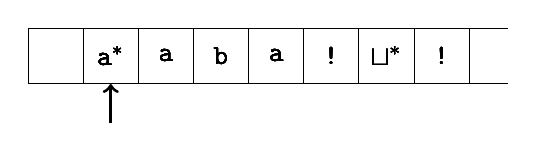
\begin{tikzpicture}

\draw (0.35, 0.35)
  node[draw, line width=0.01cm, , color=black,
       rounded corners=0cm, inner sep=0cm] {

\begin{minipage}[t][0.7cm]{0.7cm}
\mbox{}

\end{minipage}

};\draw (0.35, 0.35) node[color=black] {\texttt{\DOLLAR}};
\draw (1.0499999999999998, 0.35)
  node[draw, line width=0.01cm, , color=black,
       rounded corners=0cm, inner sep=0cm] {

\begin{minipage}[t][0.7cm]{0.7cm}
\mbox{}

\end{minipage}

};\draw (1.0499999999999998, 0.35) node[color=black] {\texttt{a$^*$}};
\draw (1.7499999999999998, 0.35)
  node[draw, line width=0.01cm, , color=black,
       rounded corners=0cm, inner sep=0cm] {

\begin{minipage}[t][0.7cm]{0.7cm}
\mbox{}

\end{minipage}

};\draw (1.7499999999999998, 0.35) node[color=black] {\texttt{a}};
\draw (2.4499999999999997, 0.35)
  node[draw, line width=0.01cm, , color=black,
       rounded corners=0cm, inner sep=0cm] {

\begin{minipage}[t][0.7cm]{0.7cm}
\mbox{}

\end{minipage}

};\draw (2.4499999999999997, 0.35) node[color=black] {\texttt{b}};
\draw (3.15, 0.35)
  node[draw, line width=0.01cm, , color=black,
       rounded corners=0cm, inner sep=0cm] {

\begin{minipage}[t][0.7cm]{0.7cm}
\mbox{}

\end{minipage}

};\draw (3.15, 0.35) node[color=black] {\texttt{a}};
\draw (3.85, 0.35)
  node[draw, line width=0.01cm, , color=black,
       rounded corners=0cm, inner sep=0cm] {

\begin{minipage}[t][0.7cm]{0.7cm}
\mbox{}

\end{minipage}

};\draw (3.85, 0.35) node[color=black] {\texttt{!}};
\draw (4.550000000000001, 0.35)
  node[draw, line width=0.01cm, , color=black,
       rounded corners=0cm, inner sep=0cm] {

\begin{minipage}[t][0.7cm]{0.7cm}
\mbox{}

\end{minipage}

};\draw (4.550000000000001, 0.35) node[color=black] {\texttt{$\sqcup^*$}};
\draw (5.25, 0.35)
  node[draw, line width=0.01cm, , color=black,
       rounded corners=0cm, inner sep=0cm] {

\begin{minipage}[t][0.7cm]{0.7cm}
\mbox{}

\end{minipage}

};\draw (5.25, 0.35) node[color=black] {\texttt{!}};
\draw (0.35, 0.35)
  node[draw, line width=0.01cm, , color=black,
       rounded corners=0cm, inner sep=0cm] {

\begin{minipage}[t][0.7cm]{0.7cm}
\mbox{}

\end{minipage}

};\draw (0.35, 0.35) node[color=black] {\texttt{\DOLLAR}};
\draw (1.0499999999999998, 0.35)
  node[draw, line width=0.01cm, , color=black,
       rounded corners=0cm, inner sep=0cm] {

\begin{minipage}[t][0.7cm]{0.7cm}
\mbox{}

\end{minipage}

};\draw (1.0499999999999998, 0.35) node[color=black] {\texttt{a$^*$}};
\draw (1.7499999999999998, 0.35)
  node[draw, line width=0.01cm, , color=black,
       rounded corners=0cm, inner sep=0cm] {

\begin{minipage}[t][0.7cm]{0.7cm}
\mbox{}

\end{minipage}

};\draw (1.7499999999999998, 0.35) node[color=black] {\texttt{a}};
\draw (2.4499999999999997, 0.35)
  node[draw, line width=0.01cm, , color=black,
       rounded corners=0cm, inner sep=0cm] {

\begin{minipage}[t][0.7cm]{0.7cm}
\mbox{}

\end{minipage}

};\draw (2.4499999999999997, 0.35) node[color=black] {\texttt{b}};
\draw (3.15, 0.35)
  node[draw, line width=0.01cm, , color=black,
       rounded corners=0cm, inner sep=0cm] {

\begin{minipage}[t][0.7cm]{0.7cm}
\mbox{}

\end{minipage}

};\draw (3.15, 0.35) node[color=black] {\texttt{a}};
\draw (3.85, 0.35)
  node[draw, line width=0.01cm, , color=black,
       rounded corners=0cm, inner sep=0cm] {

\begin{minipage}[t][0.7cm]{0.7cm}
\mbox{}

\end{minipage}

};\draw (3.85, 0.35) node[color=black] {\texttt{!}};
\draw (4.550000000000001, 0.35)
  node[draw, line width=0.01cm, , color=black,
       rounded corners=0cm, inner sep=0cm] {

\begin{minipage}[t][0.7cm]{0.7cm}
\mbox{}

\end{minipage}

};\draw (4.550000000000001, 0.35) node[color=black] {\texttt{$\sqcup^*$}};
\draw (5.25, 0.35)
  node[draw, line width=0.01cm, , color=black,
       rounded corners=0cm, inner sep=0cm] {

\begin{minipage}[t][0.7cm]{0.7cm}
\mbox{}

\end{minipage}

};\draw (5.25, 0.35) node[color=black] {\texttt{!}};
\draw (0.35, 0.35)
  node[draw, line width=0.01cm, , color=black,
       rounded corners=0cm, inner sep=0cm] {

\begin{minipage}[t][0.7cm]{0.7cm}
\mbox{}

\end{minipage}

};\draw (0.35, 0.35) node[color=black] {\texttt{\DOLLAR}};
\draw (1.0499999999999998, 0.35)
  node[draw, line width=0.01cm, , color=black,
       rounded corners=0cm, inner sep=0cm] {

\begin{minipage}[t][0.7cm]{0.7cm}
\mbox{}

\end{minipage}

};\draw (1.0499999999999998, 0.35) node[color=black] {\texttt{a$^*$}};
\draw (1.7499999999999998, 0.35)
  node[draw, line width=0.01cm, , color=black,
       rounded corners=0cm, inner sep=0cm] {

\begin{minipage}[t][0.7cm]{0.7cm}
\mbox{}

\end{minipage}

};\draw (1.7499999999999998, 0.35) node[color=black] {\texttt{a}};
\draw (2.4499999999999997, 0.35)
  node[draw, line width=0.01cm, , color=black,
       rounded corners=0cm, inner sep=0cm] {

\begin{minipage}[t][0.7cm]{0.7cm}
\mbox{}

\end{minipage}

};\draw (2.4499999999999997, 0.35) node[color=black] {\texttt{b}};
\draw (3.15, 0.35)
  node[draw, line width=0.01cm, , color=black,
       rounded corners=0cm, inner sep=0cm] {

\begin{minipage}[t][0.7cm]{0.7cm}
\mbox{}

\end{minipage}

};\draw (3.15, 0.35) node[color=black] {\texttt{a}};
\draw (3.85, 0.35)
  node[draw, line width=0.01cm, , color=black,
       rounded corners=0cm, inner sep=0cm] {

\begin{minipage}[t][0.7cm]{0.7cm}
\mbox{}

\end{minipage}

};\draw (3.85, 0.35) node[color=black] {\texttt{!}};
\draw (4.550000000000001, 0.35)
  node[draw, line width=0.01cm, , color=black,
       rounded corners=0cm, inner sep=0cm] {

\begin{minipage}[t][0.7cm]{0.7cm}
\mbox{}

\end{minipage}

};\draw (4.550000000000001, 0.35) node[color=black] {\texttt{$\sqcup^*$}};
\draw (5.25, 0.35)
  node[draw, line width=0.01cm, , color=black,
       rounded corners=0cm, inner sep=0cm] {

\begin{minipage}[t][0.7cm]{0.7cm}
\mbox{}

\end{minipage}

};\draw (5.25, 0.35) node[color=black] {\texttt{!}};
\draw (0.35, 0.35)
  node[draw, line width=0.01cm, , color=black,
       rounded corners=0cm, inner sep=0cm] {

\begin{minipage}[t][0.7cm]{0.7cm}
\mbox{}

\end{minipage}

};\draw (0.35, 0.35) node[color=black] {\texttt{\DOLLAR}};
\draw (1.0499999999999998, 0.35)
  node[draw, line width=0.01cm, , color=black,
       rounded corners=0cm, inner sep=0cm] {

\begin{minipage}[t][0.7cm]{0.7cm}
\mbox{}

\end{minipage}

};\draw (1.0499999999999998, 0.35) node[color=black] {\texttt{a$^*$}};
\draw (1.7499999999999998, 0.35)
  node[draw, line width=0.01cm, , color=black,
       rounded corners=0cm, inner sep=0cm] {

\begin{minipage}[t][0.7cm]{0.7cm}
\mbox{}

\end{minipage}

};\draw (1.7499999999999998, 0.35) node[color=black] {\texttt{a}};
\draw (2.4499999999999997, 0.35)
  node[draw, line width=0.01cm, , color=black,
       rounded corners=0cm, inner sep=0cm] {

\begin{minipage}[t][0.7cm]{0.7cm}
\mbox{}

\end{minipage}

};\draw (2.4499999999999997, 0.35) node[color=black] {\texttt{b}};
\draw (3.15, 0.35)
  node[draw, line width=0.01cm, , color=black,
       rounded corners=0cm, inner sep=0cm] {

\begin{minipage}[t][0.7cm]{0.7cm}
\mbox{}

\end{minipage}

};\draw (3.15, 0.35) node[color=black] {\texttt{a}};
\draw (3.85, 0.35)
  node[draw, line width=0.01cm, , color=black,
       rounded corners=0cm, inner sep=0cm] {

\begin{minipage}[t][0.7cm]{0.7cm}
\mbox{}

\end{minipage}

};\draw (3.85, 0.35) node[color=black] {\texttt{!}};
\draw (4.550000000000001, 0.35)
  node[draw, line width=0.01cm, , color=black,
       rounded corners=0cm, inner sep=0cm] {

\begin{minipage}[t][0.7cm]{0.7cm}
\mbox{}

\end{minipage}

};\draw (4.550000000000001, 0.35) node[color=black] {\texttt{$\sqcup^*$}};
\draw (5.25, 0.35)
  node[draw, line width=0.01cm, , color=black,
       rounded corners=0cm, inner sep=0cm] {

\begin{minipage}[t][0.7cm]{0.7cm}
\mbox{}

\end{minipage}

};\draw (5.25, 0.35) node[color=black] {\texttt{!}};
\draw (0.35, 0.35)
  node[draw, line width=0.01cm, , color=black,
       rounded corners=0cm, inner sep=0cm] {

\begin{minipage}[t][0.7cm]{0.7cm}
\mbox{}

\end{minipage}

};\draw (0.35, 0.35) node[color=black] {\texttt{\DOLLAR}};
\draw (1.0499999999999998, 0.35)
  node[draw, line width=0.01cm, , color=black,
       rounded corners=0cm, inner sep=0cm] {

\begin{minipage}[t][0.7cm]{0.7cm}
\mbox{}

\end{minipage}

};\draw (1.0499999999999998, 0.35) node[color=black] {\texttt{a$^*$}};
\draw (1.7499999999999998, 0.35)
  node[draw, line width=0.01cm, , color=black,
       rounded corners=0cm, inner sep=0cm] {

\begin{minipage}[t][0.7cm]{0.7cm}
\mbox{}

\end{minipage}

};\draw (1.7499999999999998, 0.35) node[color=black] {\texttt{a}};
\draw (2.4499999999999997, 0.35)
  node[draw, line width=0.01cm, , color=black,
       rounded corners=0cm, inner sep=0cm] {

\begin{minipage}[t][0.7cm]{0.7cm}
\mbox{}

\end{minipage}

};\draw (2.4499999999999997, 0.35) node[color=black] {\texttt{b}};
\draw (3.15, 0.35)
  node[draw, line width=0.01cm, , color=black,
       rounded corners=0cm, inner sep=0cm] {

\begin{minipage}[t][0.7cm]{0.7cm}
\mbox{}

\end{minipage}

};\draw (3.15, 0.35) node[color=black] {\texttt{a}};
\draw (3.85, 0.35)
  node[draw, line width=0.01cm, , color=black,
       rounded corners=0cm, inner sep=0cm] {

\begin{minipage}[t][0.7cm]{0.7cm}
\mbox{}

\end{minipage}

};\draw (3.85, 0.35) node[color=black] {\texttt{!}};
\draw (4.550000000000001, 0.35)
  node[draw, line width=0.01cm, , color=black,
       rounded corners=0cm, inner sep=0cm] {

\begin{minipage}[t][0.7cm]{0.7cm}
\mbox{}

\end{minipage}

};\draw (4.550000000000001, 0.35) node[color=black] {\texttt{$\sqcup^*$}};
\draw (5.25, 0.35)
  node[draw, line width=0.01cm, , color=black,
       rounded corners=0cm, inner sep=0cm] {

\begin{minipage}[t][0.7cm]{0.7cm}
\mbox{}

\end{minipage}

};\draw (5.25, 0.35) node[color=black] {\texttt{!}};
\draw (0.35, 0.35)
  node[draw, line width=0.01cm, , color=black,
       rounded corners=0cm, inner sep=0cm] {

\begin{minipage}[t][0.7cm]{0.7cm}
\mbox{}

\end{minipage}

};\draw (0.35, 0.35) node[color=black] {\texttt{\DOLLAR}};
\draw (1.0499999999999998, 0.35)
  node[draw, line width=0.01cm, , color=black,
       rounded corners=0cm, inner sep=0cm] {

\begin{minipage}[t][0.7cm]{0.7cm}
\mbox{}

\end{minipage}

};\draw (1.0499999999999998, 0.35) node[color=black] {\texttt{a$^*$}};
\draw (1.7499999999999998, 0.35)
  node[draw, line width=0.01cm, , color=black,
       rounded corners=0cm, inner sep=0cm] {

\begin{minipage}[t][0.7cm]{0.7cm}
\mbox{}

\end{minipage}

};\draw (1.7499999999999998, 0.35) node[color=black] {\texttt{a}};
\draw (2.4499999999999997, 0.35)
  node[draw, line width=0.01cm, , color=black,
       rounded corners=0cm, inner sep=0cm] {

\begin{minipage}[t][0.7cm]{0.7cm}
\mbox{}

\end{minipage}

};\draw (2.4499999999999997, 0.35) node[color=black] {\texttt{b}};
\draw (3.15, 0.35)
  node[draw, line width=0.01cm, , color=black,
       rounded corners=0cm, inner sep=0cm] {

\begin{minipage}[t][0.7cm]{0.7cm}
\mbox{}

\end{minipage}

};\draw (3.15, 0.35) node[color=black] {\texttt{a}};
\draw (3.85, 0.35)
  node[draw, line width=0.01cm, , color=black,
       rounded corners=0cm, inner sep=0cm] {

\begin{minipage}[t][0.7cm]{0.7cm}
\mbox{}

\end{minipage}

};\draw (3.85, 0.35) node[color=black] {\texttt{!}};
\draw (4.550000000000001, 0.35)
  node[draw, line width=0.01cm, , color=black,
       rounded corners=0cm, inner sep=0cm] {

\begin{minipage}[t][0.7cm]{0.7cm}
\mbox{}

\end{minipage}

};\draw (4.550000000000001, 0.35) node[color=black] {\texttt{$\sqcup^*$}};
\draw (5.25, 0.35)
  node[draw, line width=0.01cm, , color=black,
       rounded corners=0cm, inner sep=0cm] {

\begin{minipage}[t][0.7cm]{0.7cm}
\mbox{}

\end{minipage}

};\draw (5.25, 0.35) node[color=black] {\texttt{!}};
\draw (0.35, 0.35)
  node[draw, line width=0.01cm, , color=black,
       rounded corners=0cm, inner sep=0cm] {

\begin{minipage}[t][0.7cm]{0.7cm}
\mbox{}

\end{minipage}

};\draw (0.35, 0.35) node[color=black] {\texttt{\DOLLAR}};
\draw (1.0499999999999998, 0.35)
  node[draw, line width=0.01cm, , color=black,
       rounded corners=0cm, inner sep=0cm] {

\begin{minipage}[t][0.7cm]{0.7cm}
\mbox{}

\end{minipage}

};\draw (1.0499999999999998, 0.35) node[color=black] {\texttt{a$^*$}};
\draw (1.7499999999999998, 0.35)
  node[draw, line width=0.01cm, , color=black,
       rounded corners=0cm, inner sep=0cm] {

\begin{minipage}[t][0.7cm]{0.7cm}
\mbox{}

\end{minipage}

};\draw (1.7499999999999998, 0.35) node[color=black] {\texttt{a}};
\draw (2.4499999999999997, 0.35)
  node[draw, line width=0.01cm, , color=black,
       rounded corners=0cm, inner sep=0cm] {

\begin{minipage}[t][0.7cm]{0.7cm}
\mbox{}

\end{minipage}

};\draw (2.4499999999999997, 0.35) node[color=black] {\texttt{b}};
\draw (3.15, 0.35)
  node[draw, line width=0.01cm, , color=black,
       rounded corners=0cm, inner sep=0cm] {

\begin{minipage}[t][0.7cm]{0.7cm}
\mbox{}

\end{minipage}

};\draw (3.15, 0.35) node[color=black] {\texttt{a}};
\draw (3.85, 0.35)
  node[draw, line width=0.01cm, , color=black,
       rounded corners=0cm, inner sep=0cm] {

\begin{minipage}[t][0.7cm]{0.7cm}
\mbox{}

\end{minipage}

};\draw (3.85, 0.35) node[color=black] {\texttt{!}};
\draw (4.550000000000001, 0.35)
  node[draw, line width=0.01cm, , color=black,
       rounded corners=0cm, inner sep=0cm] {

\begin{minipage}[t][0.7cm]{0.7cm}
\mbox{}

\end{minipage}

};\draw (4.550000000000001, 0.35) node[color=black] {\texttt{$\sqcup^*$}};
\draw (5.25, 0.35)
  node[draw, line width=0.01cm, , color=black,
       rounded corners=0cm, inner sep=0cm] {

\begin{minipage}[t][0.7cm]{0.7cm}
\mbox{}

\end{minipage}

};\draw (5.25, 0.35) node[color=black] {\texttt{!}};
\draw (0.35, 0.35)
  node[draw, line width=0.01cm, , color=black,
       rounded corners=0cm, inner sep=0cm] {

\begin{minipage}[t][0.7cm]{0.7cm}
\mbox{}

\end{minipage}

};\draw (0.35, 0.35) node[color=black] {\texttt{\DOLLAR}};
\draw (1.0499999999999998, 0.35)
  node[draw, line width=0.01cm, , color=black,
       rounded corners=0cm, inner sep=0cm] {

\begin{minipage}[t][0.7cm]{0.7cm}
\mbox{}

\end{minipage}

};\draw (1.0499999999999998, 0.35) node[color=black] {\texttt{a$^*$}};
\draw (1.7499999999999998, 0.35)
  node[draw, line width=0.01cm, , color=black,
       rounded corners=0cm, inner sep=0cm] {

\begin{minipage}[t][0.7cm]{0.7cm}
\mbox{}

\end{minipage}

};\draw (1.7499999999999998, 0.35) node[color=black] {\texttt{a}};
\draw (2.4499999999999997, 0.35)
  node[draw, line width=0.01cm, , color=black,
       rounded corners=0cm, inner sep=0cm] {

\begin{minipage}[t][0.7cm]{0.7cm}
\mbox{}

\end{minipage}

};\draw (2.4499999999999997, 0.35) node[color=black] {\texttt{b}};
\draw (3.15, 0.35)
  node[draw, line width=0.01cm, , color=black,
       rounded corners=0cm, inner sep=0cm] {

\begin{minipage}[t][0.7cm]{0.7cm}
\mbox{}

\end{minipage}

};\draw (3.15, 0.35) node[color=black] {\texttt{a}};
\draw (3.85, 0.35)
  node[draw, line width=0.01cm, , color=black,
       rounded corners=0cm, inner sep=0cm] {

\begin{minipage}[t][0.7cm]{0.7cm}
\mbox{}

\end{minipage}

};\draw (3.85, 0.35) node[color=black] {\texttt{!}};
\draw (4.550000000000001, 0.35)
  node[draw, line width=0.01cm, , color=black,
       rounded corners=0cm, inner sep=0cm] {

\begin{minipage}[t][0.7cm]{0.7cm}
\mbox{}

\end{minipage}

};\draw (4.550000000000001, 0.35) node[color=black] {\texttt{$\sqcup^*$}};
\draw (5.25, 0.35)
  node[draw, line width=0.01cm, , color=black,
       rounded corners=0cm, inner sep=0cm] {

\begin{minipage}[t][0.7cm]{0.7cm}
\mbox{}

\end{minipage}

};\draw (5.25, 0.35) node[color=black] {\texttt{!}};\draw[line width=0.01cm,black] (5.6000000000000005,0.7) to  (6.1000000000000005,0.7);
\draw[line width=0.01cm,black] (5.6000000000000005,0.0) to  (6.1000000000000005,0.0);
\draw[line width=0.04cm,black,->] (1.05,-0.51) to  (1.05,-0.01);
\end{tikzpicture}

\end{center}


Note the traversal pattern:
{\small \begin{console}[frame=single,fontsize=\small]
[student@localhost 350-hashtable] g++ main.cpp; ./a.out
hash of
42: 42
42: 42
-1: 18446744073709551615
3.14: 5464867211497793177
0.0: 6369015886390043782
'a': 97
true: 1
"hello world": 5577293430985752569
\end{console}
}


For
\begin{center}
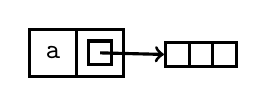
\begin{tikzpicture}

\draw (0.3, 0.3)
  node[draw, line width=0.04cm, , color=black,
       rounded corners=0cm, inner sep=0cm] {

\begin{minipage}[t][0.6cm]{0.6cm}
\mbox{}

\end{minipage}

};\draw (0.3, 0.3) node[color=black] {{\texttt{a}}};
\draw (0.8999999999999999, 0.3)
  node[draw, line width=0.04cm, , color=black,
       rounded corners=0cm, inner sep=0cm] {

\begin{minipage}[t][0.6cm]{0.6cm}
\mbox{}

\end{minipage}

};
\draw (0.9, 0.3)
  node[draw, line width=0.04cm, , color=black,
       rounded corners=0cm, inner sep=0cm] {

\begin{minipage}[t][0.3cm]{0.3cm}
\mbox{}

\end{minipage}

};
\draw (1.88, 0.28)
  node[draw, line width=0.04cm, , color=black,
       rounded corners=0cm, inner sep=0cm] {

\begin{minipage}[t][0.3cm]{0.3cm}
\mbox{}

\end{minipage}

};
\draw (2.1799999999999997, 0.28)
  node[draw, line width=0.04cm, , color=black,
       rounded corners=0cm, inner sep=0cm] {

\begin{minipage}[t][0.3cm]{0.3cm}
\mbox{}

\end{minipage}

};
\draw (2.48, 0.28)
  node[draw, line width=0.04cm, , color=black,
       rounded corners=0cm, inner sep=0cm] {

\begin{minipage}[t][0.3cm]{0.3cm}
\mbox{}

\end{minipage}

};\draw[line width=0.04cm,black,->] (0.9,0.3) to  (1.71,0.28);
\end{tikzpicture}

\end{center}


we are looking for a variable $V$ such that
\[
  V \rightarrow XY \text{ where } X \in \{B,C\}, Y \in \{S\}
\]
There is no such $V$.
For
\begin{center}
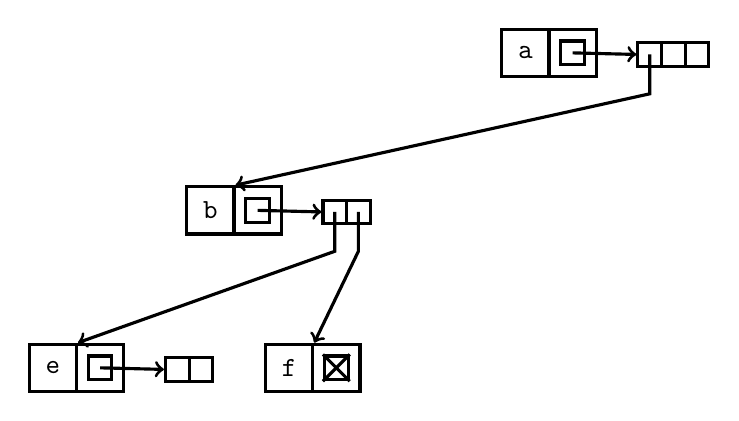
\begin{tikzpicture}

\draw (0.3, 0.3)
  node[draw, line width=0.04cm, , color=black,
       rounded corners=0cm, inner sep=0cm] {

\begin{minipage}[t][0.6cm]{0.6cm}
\mbox{}

\end{minipage}

};\draw (0.3, 0.3) node[color=black] {{\texttt{a}}};
\draw (0.8999999999999999, 0.3)
  node[draw, line width=0.04cm, , color=black,
       rounded corners=0cm, inner sep=0cm] {

\begin{minipage}[t][0.6cm]{0.6cm}
\mbox{}

\end{minipage}

};
\draw (0.9, 0.3)
  node[draw, line width=0.04cm, , color=black,
       rounded corners=0cm, inner sep=0cm] {

\begin{minipage}[t][0.3cm]{0.3cm}
\mbox{}

\end{minipage}

};
\draw (1.88, 0.28)
  node[draw, line width=0.04cm, , color=black,
       rounded corners=0cm, inner sep=0cm] {

\begin{minipage}[t][0.3cm]{0.3cm}
\mbox{}

\end{minipage}

};
\draw (2.1799999999999997, 0.28)
  node[draw, line width=0.04cm, , color=black,
       rounded corners=0cm, inner sep=0cm] {

\begin{minipage}[t][0.3cm]{0.3cm}
\mbox{}

\end{minipage}

};
\draw (2.48, 0.28)
  node[draw, line width=0.04cm, , color=black,
       rounded corners=0cm, inner sep=0cm] {

\begin{minipage}[t][0.3cm]{0.3cm}
\mbox{}

\end{minipage}

};\draw[line width=0.04cm,black,->] (0.9,0.3) to  (1.71,0.28);

\draw (-3.6999999999999997, -1.7)
  node[draw, line width=0.04cm, , color=black,
       rounded corners=0cm, inner sep=0cm] {

\begin{minipage}[t][0.6cm]{0.6cm}
\mbox{}

\end{minipage}

};\draw (-3.6999999999999997, -1.7) node[color=black] {{\texttt{b}}};
\draw (-3.0999999999999996, -1.7)
  node[draw, line width=0.04cm, , color=black,
       rounded corners=0cm, inner sep=0cm] {

\begin{minipage}[t][0.6cm]{0.6cm}
\mbox{}

\end{minipage}

};
\draw (-3.0999999999999996, -1.7)
  node[draw, line width=0.04cm, , color=black,
       rounded corners=0cm, inner sep=0cm] {

\begin{minipage}[t][0.3cm]{0.3cm}
\mbox{}

\end{minipage}

};
\draw (-2.12, -1.7200000000000002)
  node[draw, line width=0.04cm, , color=black,
       rounded corners=0cm, inner sep=0cm] {

\begin{minipage}[t][0.3cm]{0.3cm}
\mbox{}

\end{minipage}

};
\draw (-1.8199999999999998, -1.7200000000000002)
  node[draw, line width=0.04cm, , color=black,
       rounded corners=0cm, inner sep=0cm] {

\begin{minipage}[t][0.3cm]{0.3cm}
\mbox{}

\end{minipage}

};\draw[line width=0.04cm,black,->] (-3.1,-1.7) to  (-2.29,-1.72);

\draw (-5.7, -3.6999999999999997)
  node[draw, line width=0.04cm, , color=black,
       rounded corners=0cm, inner sep=0cm] {

\begin{minipage}[t][0.6cm]{0.6cm}
\mbox{}

\end{minipage}

};\draw (-5.7, -3.6999999999999997) node[color=black] {{\texttt{e}}};
\draw (-5.1, -3.6999999999999997)
  node[draw, line width=0.04cm, , color=black,
       rounded corners=0cm, inner sep=0cm] {

\begin{minipage}[t][0.6cm]{0.6cm}
\mbox{}

\end{minipage}

};
\draw (-5.1, -3.7)
  node[draw, line width=0.04cm, , color=black,
       rounded corners=0cm, inner sep=0cm] {

\begin{minipage}[t][0.3cm]{0.3cm}
\mbox{}

\end{minipage}

};
\draw (-4.119999999999999, -3.72)
  node[draw, line width=0.04cm, , color=black,
       rounded corners=0cm, inner sep=0cm] {

\begin{minipage}[t][0.3cm]{0.3cm}
\mbox{}

\end{minipage}

};
\draw (-3.8199999999999994, -3.72)
  node[draw, line width=0.04cm, , color=black,
       rounded corners=0cm, inner sep=0cm] {

\begin{minipage}[t][0.3cm]{0.3cm}
\mbox{}

\end{minipage}

};\draw[line width=0.04cm,black,->] (-5.1,-3.7) to  (-4.29,-3.72);

\draw (-2.7, -3.6999999999999997)
  node[draw, line width=0.04cm, , color=black,
       rounded corners=0cm, inner sep=0cm] {

\begin{minipage}[t][0.6cm]{0.6cm}
\mbox{}

\end{minipage}

};\draw (-2.7, -3.6999999999999997) node[color=black] {{\texttt{f}}};
\draw (-2.1, -3.6999999999999997)
  node[draw, line width=0.04cm, , color=black,
       rounded corners=0cm, inner sep=0cm] {

\begin{minipage}[t][0.6cm]{0.6cm}
\mbox{}

\end{minipage}

};
\draw (-2.1, -3.7)
  node[draw, line width=0.04cm, , color=black,
       rounded corners=0cm, inner sep=0cm] {

\begin{minipage}[t][0.3cm]{0.3cm}
\mbox{}

\end{minipage}

};\draw[line width=0.04cm,black] (-2.27,-3.53) to  (-1.93,-3.87);
\draw[line width=0.04cm,black] (-1.93,-3.53) to  (-2.27,-3.87);
\draw[line width=0.04cm,black,->] (1.88,0.28) to  (1.88,-0.22) to  (-3.38,-1.38);
\draw[line width=0.04cm,black,->] (-2.12,-1.72) to  (-2.12,-2.22) to  (-5.38,-3.38);
\draw[line width=0.04cm,black,->] (-1.82,-1.72) to  (-1.82,-2.22) to  (-2.38,-3.38);
\end{tikzpicture}

\end{center}


since there are no variables at $(2, 1)$, we don't have any $V$'s to add to $(4,1)$.
For

\begin{center}
\begin{tikzpicture}[>=triangle 60,shorten >=0.5pt,node distance=2cm,auto,initial text=, double distance=2pt]
\node[state] (A) at (  0,  0) {$\{q_0\}$};
\node[state] (B) at (  3,  0) {$\{\}$};

\path[->]

;
\end{tikzpicture}
\end{center}
    

we want $V$ such that $V \rightarrow AA$. There's only one case: $V = C$.
Altogether we have

\begin{longtable}{|r||r|r|r|r|r|}
\hline 
         & $w_1$ & $w_2$ & $w_3$ & $w_4$ & $\ldots$ \\ \hline \hline 
$M_1$    &       &       &       &       &          \\ \hline 
$M_2$    &       &       &       &       &          \\ \hline 
$M_3$    &       &       &       &       &          \\ \hline 
$M_4$    &       &       &       &       &          \\ \hline 
$\ldots$ &       &       &       &       &          \\ \hline 
\end{longtable}
        


For entry (4,2) you should get:

\begin{longtable}{|r||r|r|r|r|r|}
\hline 
         & $w_1$ & $w_2$ & $w_3$ & $w_4$ & $\ldots$ \\ \hline \hline 
$M_1$    & 0     & 0     & 1     & 0     & ...      \\ \hline 
$M_2$    & 1     & 0     & 1     & 1     & ...      \\ \hline 
$M_3$    & 0     & 1     & 1     & 1     & ...      \\ \hline 
$M_4$    & 1     & 0     & 1     & 1     & ...      \\ \hline 
$\ldots$ &       &       &       &       &          \\ \hline 
\end{longtable}
        


For entry (4,3) you should get:
\begin{center}
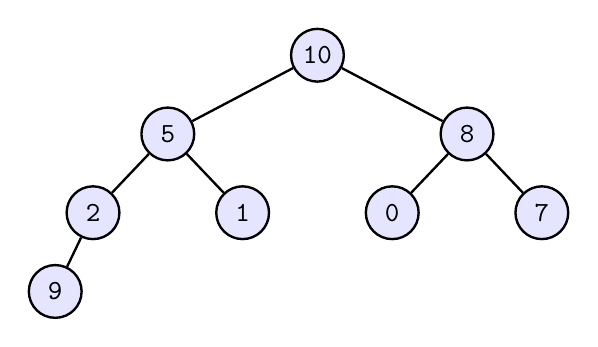
\begin{tikzpicture}

\fill[blue!10] (0.0, 0.0) circle (0.35);
\node [line width=0.03cm,black,minimum size=0.6699999999999999cm,draw,circle] at (0.0,0.0)(10){};\draw (0.0, 0.0) node[color=black] {\texttt{10}};
\fill[blue!10] (-1.9, -1.0) circle (0.35);
\node [line width=0.03cm,black,minimum size=0.6699999999999999cm,draw,circle] at (-1.9,-1.0)(5){};\draw (-1.9, -1.0) node[color=black] {\texttt{5}};
\fill[blue!10] (1.9, -1.0) circle (0.35);
\node [line width=0.03cm,black,minimum size=0.6699999999999999cm,draw,circle] at (1.9,-1.0)(8){};\draw (1.9, -1.0) node[color=black] {\texttt{8}};
\fill[blue!10] (-2.85, -2.0) circle (0.35);
\node [line width=0.03cm,black,minimum size=0.6699999999999999cm,draw,circle] at (-2.85,-2.0)(2){};\draw (-2.85, -2.0) node[color=black] {\texttt{2}};
\fill[blue!10] (-0.95, -2.0) circle (0.35);
\node [line width=0.03cm,black,minimum size=0.6699999999999999cm,draw,circle] at (-0.95,-2.0)(1){};\draw (-0.95, -2.0) node[color=black] {\texttt{1}};
\fill[blue!10] (0.95, -2.0) circle (0.35);
\node [line width=0.03cm,black,minimum size=0.6699999999999999cm,draw,circle] at (0.95,-2.0)(0){};\draw (0.95, -2.0) node[color=black] {\texttt{0}};
\fill[blue!10] (2.85, -2.0) circle (0.35);
\node [line width=0.03cm,black,minimum size=0.6699999999999999cm,draw,circle] at (2.85,-2.0)(7){};\draw (2.85, -2.0) node[color=black] {\texttt{7}};
\fill[blue!10] (-3.33, -3.0) circle (0.35);
\node [line width=0.03cm,black,minimum size=0.6699999999999999cm,draw,circle] at (-3.33,-3.0)(9){};\draw (-3.33, -3.0) node[color=black] {\texttt{9}};\draw[line width=0.03cm,black] (10) to  (5);
\draw[line width=0.03cm,black] (10) to  (8);
\draw[line width=0.03cm,black] (5) to  (2);
\draw[line width=0.03cm,black] (5) to  (1);
\draw[line width=0.03cm,black] (8) to  (0);
\draw[line width=0.03cm,black] (8) to  (7);
\draw[line width=0.03cm,black] (2) to  (9);
\end{tikzpicture}

\end{center}



\underline{Fifth Row}:

\begin{center}
\begin{tikzpicture}[>=triangle 60,shorten >=0.5pt,node distance=2cm,auto,initial text=, double distance=2pt]
\node[state,initial] (A) at (  0,  0) {$\{q_0\}$};
\node[state] (B) at (  3,  0) {$\{\}$};

\path[->]
(A) edge [bend left=0,pos=0.5,above] node {$a,b$} (B)
(B) edge [loop above] node {$a,b$} ()

;
\end{tikzpicture}
\end{center}
    

At $(5, 1)$ we use $S \rightarrow AC$ and at $(5,2)$ we use $B \rightarrow CB$.

\underline{Sixth Row}.
Using the following traversal shown, you should get the following entry for (6,1):
... and we're done!!! Here's the final table:

\begin{center}
\begin{tikzpicture}[>=triangle 60,shorten >=0.5pt,node distance=2cm,auto,initial text=, double distance=2pt]
\node[state,initial] (A) at (  0,  0) {};

\path[->]
(A) edge [loop above] node {$a,b$} ()

;
\end{tikzpicture}
\end{center}
    


So what have we achieved? First of all $S$ is in the entry at $(6,1)$.
What does this mean? 
Recall again that this means $S$ can derive $w_{1,6}$, which is the
string we started with, i.e. $baaaab$.
Secondly, you can write down the productions that derive $baaaab$ from $S$.
Can you write them down using the table? [SPOILERS AHEAD ...]

Of course CYK gives you even more.
For instance we also know that $B$ is also in the entry at (6,1).
This means that $B$ can also derive $baaab$.
If you look at the entry at (2,5), you conclude that $B$ can derive $aaab$.
In other words besides addressing the question of whether $baaaab$ can be
generated by the grammar, we have also answered the question for all
substrings of $baaaab$.
Make sure you see this.

OK ... so you know that $S$ can derive $baaaab$ (i.e.
$baaaab \in L(G)$ for the above CFG $G$).
But what is the derivation?
If you've understood the mathematical reasoning so far,
you should have no problems writing down the derivation.
\newcommand\ddd{&\implies}
\begin{align*}
  S_{(3,1)(3,4)}
  &\implies A_{(1,1)(2,2)} \cdot B_{(2,4)(1,6)} \\
  &\implies B_b \cdot C_{(1,2)(1,3)} \cdot B_{(2,4)(1,6)} & & \text{(or $C_b$ instead of $B_b$)} \\
  &\implies b \cdot C_{(1,2)(1,3)} \cdot B_{(2,4)(1,6)} \\
  &\implies b \cdot A_a \cdot A_a \cdot B_{(2,4)(1,6)} \\
  &\implies b \cdot a \cdot A_a \cdot B_{(2,4)(1,6)} \\
  &\implies b \cdot a \cdot a \cdot B_{(2,4)(1,6)} \\
  &\implies b \cdot a \cdot a \cdot C_{(1,4)(1,5)} \cdot B_b & &  \text{(or $C_b$ instead of $B_b$)} \\
  &\implies b \cdot a \cdot a \cdot A_a \cdot A_a \cdot B_b \\
  &\implies b \cdot a \cdot a \cdot a \cdot A_a \cdot B_b \\
  &\implies b \cdot a \cdot a \cdot a \cdot a \cdot B_b \\
  &\implies b \cdot a \cdot a \cdot a \cdot a \cdot b
\end{align*}

Note that if you are only interested in whether $baaaab$ is generated by the grammar
(and not the actual derivation), then you only need to fill the CYK table in
the following way:
\begin{console}[frame=single,fontsize=\footnotesize]
[student@localhost forward_list] g++ main.cpp; ./a.out
1.
true
size: 0
[3, 2, 1, 0]
[]
2.
[1, 2, 3, 4]
[2, 3, 4]
3.
[1, 2, 3, 4]
42
[42, 2, 3, 4]
4.
[1, 2, 3, 4]
[1, 2, 4]
5.
[1, 2, 3, 4]
[1, 2]
6.
[1, 2, 3, 4]
[1, 2, 77777, 88888, 99999, 3, 4]
7.
[1, 2, 3, 4]
[1, 2, -1, -1, -1, -1, -1, 3, 4]
8.
[1, 2, 3, 4]
[1, 2, 88, 99, 3, 4]
\end{console}



The CYK algorithm requires us to fill data into half of an $n$--by--$n$
array -- there are altogether $(1/2)n^2$ cells to fill.
Each cell $X$ of the array requires us to go through at most $n$ pairs
of cells which are already fill and see if we can find a production rule
that can help in filling cell $X$.
(We can speed up the search for a suitable production rule
if we find a suitable organization for the collection
of production rules. Which one?)
Therefore the total runtime is $O(n^3)$.
The space complexity is of course $\Theta(n^2)$.
(If you want to take into account the grammar, then the runtime is
$O(n^3 |G|)$ where $|G|$ is the size of the grammar
which is the total count of all symbols that appear
in all the production rules.)


\begin{ex} 
  \label{ex:some-decision1}
  \tinysidebar{\debug{exercises/{empty0/question.tex}}}
  \solutionlink{sol:some-decision1}
  \qed
\end{ex} 
\begin{python0}
from solutions import *
add(label="ex:some-decision1",
    srcfilename='exercises/some-decision1/answer.tex') 
\end{python0}



\begin{ex} 
  \label{ex:some-decision1}
  \tinysidebar{\debug{exercises/{empty0/question.tex}}}
  \solutionlink{sol:some-decision1}
  \qed
\end{ex} 
\begin{python0}
from solutions import *
add(label="ex:some-decision1",
    srcfilename='exercises/some-decision1/answer.tex') 
\end{python0}



\begin{ex} 
  \label{ex:some-decision1}
  \tinysidebar{\debug{exercises/{empty0/question.tex}}}
  \solutionlink{sol:some-decision1}
  \qed
\end{ex} 
\begin{python0}
from solutions import *
add(label="ex:some-decision1",
    srcfilename='exercises/some-decision1/answer.tex') 
\end{python0}



\begin{ex} 
  \label{ex:some-decision1}
  \tinysidebar{\debug{exercises/{empty0/question.tex}}}
  \solutionlink{sol:some-decision1}
  \qed
\end{ex} 
\begin{python0}
from solutions import *
add(label="ex:some-decision1",
    srcfilename='exercises/some-decision1/answer.tex') 
\end{python0}


1. 
\begin{console}[frame=single,fontsize=\footnotesize]
[student@localhost list] g++ main.cpp; ./a.out
1.
true
size: 0
[1, 0, 111, 222]
2.
[1, 2, 3, 4]
[2, 3]
3.
[1, 2, 3, 4]
[111, 2, 3, 999]
4.
[1, 2, 3, 4]
[1, 3, 4]
[1, 3, 4]
5.
[1, 2, 3, 4]
[1, 4]
6.
[1, 2, 3, 4]
[1, 99999, 88888, 77777, 2, 3, 4]
7.
[1, 2, 3, 4]
[1, -1, -1, -1, -1, -1, 2, 3, 4]
8.
[1, 2, 3, 4]
[1, 88, 99, 2, 3, 4]
9.
[1, 2, 3, 4]
4 3 2 1
\end{console}


The derivations are
\begin{align*}
  S \implies AA \implies aA \implies aa \\
  S \implies AB \implies aB \implies aa \\
  S \implies BA \implies aA \implies aa \\
\end{align*}


\begin{ex} 
  \label{ex:some-decision1}
  \tinysidebar{\debug{exercises/{empty0/question.tex}}}
  \solutionlink{sol:some-decision1}
  \qed
\end{ex} 
\begin{python0}
from solutions import *
add(label="ex:some-decision1",
    srcfilename='exercises/some-decision1/answer.tex') 
\end{python0}



\begin{ex} 
  \label{ex:some-decision1}
  \tinysidebar{\debug{exercises/{empty0/question.tex}}}
  \solutionlink{sol:some-decision1}
  \qed
\end{ex} 
\begin{python0}
from solutions import *
add(label="ex:some-decision1",
    srcfilename='exercises/some-decision1/answer.tex') 
\end{python0}



\begin{ex} 
  \label{ex:some-decision1}
  \tinysidebar{\debug{exercises/{empty0/question.tex}}}
  \solutionlink{sol:some-decision1}
  \qed
\end{ex} 
\begin{python0}
from solutions import *
add(label="ex:some-decision1",
    srcfilename='exercises/some-decision1/answer.tex') 
\end{python0}

